\documentclass[12pt,brazil]{article}\usepackage[]{graphicx}\usepackage[]{xcolor}
% maxwidth is the original width if it is less than linewidth
% otherwise use linewidth (to make sure the graphics do not exceed the margin)
\makeatletter
\def\maxwidth{ %
  \ifdim\Gin@nat@width>\linewidth
    \linewidth
  \else
    \Gin@nat@width
  \fi
}
\makeatother

\definecolor{fgcolor}{rgb}{0.345, 0.345, 0.345}
\newcommand{\hlnum}[1]{\textcolor[rgb]{0.686,0.059,0.569}{#1}}%
\newcommand{\hlsng}[1]{\textcolor[rgb]{0.192,0.494,0.8}{#1}}%
\newcommand{\hlcom}[1]{\textcolor[rgb]{0.678,0.584,0.686}{\textit{#1}}}%
\newcommand{\hlopt}[1]{\textcolor[rgb]{0,0,0}{#1}}%
\newcommand{\hldef}[1]{\textcolor[rgb]{0.345,0.345,0.345}{#1}}%
\newcommand{\hlkwa}[1]{\textcolor[rgb]{0.161,0.373,0.58}{\textbf{#1}}}%
\newcommand{\hlkwb}[1]{\textcolor[rgb]{0.69,0.353,0.396}{#1}}%
\newcommand{\hlkwc}[1]{\textcolor[rgb]{0.333,0.667,0.333}{#1}}%
\newcommand{\hlkwd}[1]{\textcolor[rgb]{0.737,0.353,0.396}{\textbf{#1}}}%
\let\hlipl\hlkwb

\usepackage{framed}
\makeatletter
\newenvironment{kframe}{%
 \def\at@end@of@kframe{}%
 \ifinner\ifhmode%
  \def\at@end@of@kframe{\end{minipage}}%
  \begin{minipage}{\columnwidth}%
 \fi\fi%
 \def\FrameCommand##1{\hskip\@totalleftmargin \hskip-\fboxsep
 \colorbox{shadecolor}{##1}\hskip-\fboxsep
     % There is no \\@totalrightmargin, so:
     \hskip-\linewidth \hskip-\@totalleftmargin \hskip\columnwidth}%
 \MakeFramed {\advance\hsize-\width
   \@totalleftmargin\z@ \linewidth\hsize
   \@setminipage}}%
 {\par\unskip\endMakeFramed%
 \at@end@of@kframe}
\makeatother

\definecolor{shadecolor}{rgb}{.97, .97, .97}
\definecolor{messagecolor}{rgb}{0, 0, 0}
\definecolor{warningcolor}{rgb}{1, 0, 1}
\definecolor{errorcolor}{rgb}{1, 0, 0}
\newenvironment{knitrout}{}{} % an empty environment to be redefined in TeX

\usepackage{amsmath}
\usepackage{alltt}
\usepackage{babel}
\usepackage{color}
\usepackage{geometry}
\geometry{a4paper,landscape,left=2cm,right=2cm,top=2cm,bottom=2cm}
\newcounter{tabela}

% Adicione a linha abaixo antes do hyperref se necessário
\usepackage{url}

% Adicionando o pacote hyperref
\usepackage{hyperref}
\hypersetup{
  unicode=true,
  pdfsubject={},
  pdfkeywords={},
  plainpages=false,
  bookmarks=false,
  pdfborder={0 0 0}
}







\usepackage{fontspec}
\setmainfont{Arial}
\usepackage{float}
\usepackage{longtable}
\IfFileExists{upquote.sty}{\usepackage{upquote}}{}
\begin{document}



\begin{kframe}


{\ttfamily\noindent\bfseries\color{errorcolor}{\#\# Error in d[[v]]/d\$ncoaut: argumento não-numérico para operador binário}}\end{kframe}

\title{Produção dos Professores do PPG em XXXX da Universidade YYYY (2010-2020)}
\author{Arthur}
\date{\today}

\maketitle

\tableofcontents

\newpage

\listoftables

\clearpage

\definecolor{coautr}{rgb}{0.5,1.0,0.7}
\definecolor{ncarac}{rgb}{1,0.7,0.7}
\definecolor{ninval}{rgb}{1,1,0.5}
\definecolor{duplic}{rgb}{0.7,0.8,1}
\definecolor{capdup}{rgb}{1,0.5,1}

\section{Apresentação}

Este relatório foi produzido com scripts desenvolvidos por Jakson Alves de
Aquino\footnote{Professor do Departamento de Ciências Sociais da Universidade
Federal do Ceará (e-mail: jaa@ufc.br). Dalson Britto Figueiredo Filho, Adriano
Nervo Codato e Andréa Marcondes de Freitas contribuíram com várias sugestões
de melhorias, mas não têm nenhuma responsabilidade por eventais limitações ou
erros do software.} e disponibilizados em
\url{https://github.com/jalvesaq/PontuarLattes}.

O relatório ajuda a identificar problemas no preenchimento do Lattes pelos
professores. Cada coordenador de curso deve consultar os documentos
da sua área e ficar atento neste relatório às tabelas mais
relevantes para uma boa avaliação do seu programa.

A coautoria da produção entre professores do programa é identificada pela
coincidência de algumas informações:

\begin{itemize}

    \item Livros: ISBN e ano.

    \item Capítulos de livro: ISBN, ano e página inicial do capítulo.

    \item Artigos: ISSN, ano, volume, número do periódico e página inicial do
        artigo.

\end{itemize}

No caso de coautoria, a pontuação correspondente à publicação é dividida pelo
número de coautores que são professores do programa.

Há discussões na CAPES sobre mudanças no sistema Qualis. Entre as propostas,
está o uso do JSR ou do SNIP para a classificação da produção. Por isso, o
relatório inclui tabelas com a produção dos professores pontuadas por esses
fatores de impacto.

Vale salientar que este relatório deve ser usado com cautela porque,
embora ele seja útil para a identificação de problemas no programa de
pós-graduação, não é um instrumento usado oficialmente pela CAPES.

Observação: para cálculo da pontuação, está sendo usado Qualis
        2017-2020 não oficial, parcial e provisório que circulou nas redes
        sociais em 2019. Muitos periódicos ainda não fazem parte desse Qualis
        e, mesmo os que fazem, podem vir a ter classificação diferente na versão
        oficial.




\clearpage

\section{Data do currículo}

Na Tabela abaixo, o link para o ORCID é incluído apenas se estiver registrado
no Lattes e, as bolsas PQ do CNPq, se estiverem vigentes no dia de produção
deste relatório. Os dados das bolsas foram extraídos do site do
CNPq.\footnote{\url{http://plsql1.cnpq.br/divulg/RESULTADO_PQ_102003.curso},
acesso em 11 de março de 2021.}


\phantomsection\stepcounter{tabela}\addcontentsline{lot}{table}{Tabela \thetabela: Links para ORCID e Lattes, atualização do Currículo Lattes e bolsa PQ}
\begin{longtable}{cclrll}
    \multicolumn{6}{c}{\textbf{Tabela \thetabela: Links para ORCID e Lattes, atualização do Currículo Lattes e bolsa PQ}} \\
  \toprule
    \multicolumn{2}{c}{\textbf{Links}} & \textbf{Professor} & \textbf{Dias} &
    \multicolumn{2}{c}{\textbf{Bolsa PQ (Área)}} \\
    \midrule
\begin{kframe}


{\ttfamily\noindent\bfseries\color{errorcolor}{\#\# Error in `\$<-.data.frame`(`*tmp*`, areap, value = "{}()"{}): replacement has 1 row, data has 0}}\end{kframe}\href{}{\includegraphics[width=4mm]{orcid.png}} & \href{http://lattes.cnpq.br/}{\includegraphics[width=4mm]{lattes.png}} \\


\bottomrule
\end{longtable}

\clearpage

\section{Títulos e prêmios}

\phantomsection\stepcounter{tabela}\addcontentsline{lot}{table}{Tabela \thetabela: Curso de doutorado}
\begin{ltabulary}{LLLcc}
\multicolumn{5}{c}{\textbf{Tabela \thetabela: Curso de doutorado}} \\
  \toprule
\textbf{Professor} & \textbf{Instituição doutorado} & \textbf{Nome do curso} & \textbf{Ano} & \textbf{Tempo} \\
\midrule
\endfirsthead
  \toprule
\textbf{Professor} & \textbf{Instituição doutorado} & \textbf{Nome do curso} & \textbf{Ano} & \textbf{Tempo} \\
\midrule
\endhead
\midrule
\multicolumn{5}{r}{{\footnotesize Continua na próxima página}} \\
\endfoot
\bottomrule
\endlastfoot
Paulo César Borges Alves & University of Liverpool & Social And Environmental Studies Sociology & 1990 & 34 \\
Miriam Cristina Marcilio Rabelo & University of Liverpool & Ciências Sociais/ Antropologia & 1990 & 34 \\
Eduardo Paes Machado & UNICAMP & Ciências Sociais & 1992 & 32 \\
Iracema Brandão Guimarães & USP & Sociologia & 1994 & 30 \\
Antonio da Silva Camara & Université Paris Diderot & Sociologia & 1994 & 30 \\
Maria da Graça Druck de Faria & UNICAMP & Programa de Pós Graduação em Ciências Sociais & 1995 & 29 \\
Elisio Guerreiro do Estanque & Universidade de Coimbra & Sociologia & 1999 & 25 \\
Iara Maria de Almeida Souza & UFBA & Ciências Sociais & 2004 & 20 \\
Maria Gabriela Hita & UNICAMP & Ciências Sociais & 2004 & 20 \\
Clóvis Roberto Zimmermann & Ruprecht-Karls-Universität Heidelberg & Sociologia & 2004 & 20 \\
Luiz Claudio Lourenço & IUPERJ & Ciência Política (Ciência Política e Sociologia) & 2007 & 17 \\
Jair Batista da Silva & UNICAMP & Ciências Sociais & 2008 & 16 \\
Mariana Thorstensen Possas & University of Ottawa & Criminologia & 2009 & 15 \\
Leonardo Fernandes Nascimento & UERJ & Sociologia & 2013 & 11 \\
Alan Delazeri Mocellim & USP & Sociologia & 2014 & 10 \\
Ricardo Pagliuso Regatieri & USP & Sociologia & 2015 & 9 \\
Sue Angélica Serra Iamamoto & Queen Mary University of London & Ciência Política & 2016 & 8 \\
Rafael de Aguiar Arantes & UFBA & Ciências Sociais & 2016 & 8 \\
Felipe Vargas & UFRGS & Programa de Pós-Graduação em Sociologia & 2017 & 7 \\
Lucas Amaral de Oliveira & USP & Sociologia & 2018 & 6 \\
Ana Rodrigues Cavalcanti Alves & UFPE & Sociologia & 2018 & 6 \\
Débora Previatti & UFSC & Sociologia Política & 2019 & 5 \\
Bruno Costa Barreiros & UFSC & Sociologia Política & 2019 & 5 \\
\hline \multicolumn{4}{l}{Tempo mediano de titulação}  &  16 \\
\multicolumn{4}{l}{Tempo médio de titulação}  &  17 \\
\end{ltabulary}

\newpage


\phantomsection\stepcounter{tabela}\addcontentsline{lot}{table}{Tabela \thetabela: Área de titulação}
\begin{ltabulary}{Lrr}
\multicolumn{3}{c}{\textbf{Tabela \thetabela: Área de titulação}} \\
  \toprule
\textbf{Nome do curso} & \textbf{Frequência} & \textbf{\%} \\
\midrule
\endfirsthead
\multicolumn{3}{c}{{\footnotesize ... continuação da página anterior}} \\
  \toprule
\textbf{Nome do curso} & \textbf{Frequência} & \textbf{\%} \\
\midrule
\endhead
\midrule
\multicolumn{3}{r}{{\footnotesize Continua na próxima página}} \\
\endfoot
\bottomrule
\endlastfoot
Sociologia & 9 & 39,1 \\
Ciências Sociais & 5 & 21,7 \\
Sociologia Política & 2 & 8,7 \\
Ciência Política & 1 & 4,3 \\
Ciência Política (Ciência Política e Sociologia) & 1 & 4,3 \\
Ciências Sociais/ Antropologia & 1 & 4,3 \\
Criminologia & 1 & 4,3 \\
Programa de Pós-Graduação em Sociologia & 1 & 4,3 \\
Programa de Pós Graduação em Ciências Sociais & 1 & 4,3 \\
Social And Environmental Studies Sociology & 1 & 4,3 \\
\hline Total & 23 & 100,0 \\
\end{ltabulary}


\newpage

\phantomsection\stepcounter{tabela}\addcontentsline{lot}{table}{Tabela \thetabela: Instituição doutorado}
\begin{ltabulary}{Lrr}
\multicolumn{3}{c}{\textbf{Tabela \thetabela: Instituição doutorado}} \\
  \toprule
\textbf{Instituição} & \textbf{Frequência} & \textbf{\%} \\
\midrule
\endfirsthead
\multicolumn{3}{c}{{\footnotesize ... continuação da página anterior}} \\
  \toprule
\textbf{Instituição} & \textbf{Frequência} & \textbf{\%} \\
\midrule
\endhead
\midrule
\multicolumn{3}{r}{{\footnotesize Continua na próxima página}} \\
\endfoot
\bottomrule
\endlastfoot
UNICAMP & 4 & 17,4 \\
USP & 4 & 17,4 \\
UFBA & 2 & 8,7 \\
UFSC & 2 & 8,7 \\
University of Liverpool & 2 & 8,7 \\
IUPERJ & 1 & 4,3 \\
Queen Mary University of London & 1 & 4,3 \\
Ruprecht-Karls-Universität Heidelberg & 1 & 4,3 \\
UERJ & 1 & 4,3 \\
UFPE & 1 & 4,3 \\
UFRGS & 1 & 4,3 \\
Universidade de Coimbra & 1 & 4,3 \\
Université Paris Diderot & 1 & 4,3 \\
University of Ottawa & 1 & 4,3 \\
\hline Total & 23 & 100,0 \\
\end{ltabulary}


\clearpage

Como pode ser visto na tabela seguinte, dos \text{23}
professores do programa, \text{0}
(\text{0}\%)
realizaram pós-doutorado pelo menos uma vez.

\begin{kframe}


{\ttfamily\noindent\bfseries\color{errorcolor}{\#\# Error in seq\_len(ncol(tab)): argumento deve ser coercível para um inteiro não-negativo}}\end{kframe}

\clearpage

\begin{kframe}


{\ttfamily\noindent\bfseries\color{errorcolor}{\#\# Error in if (nrow(premios) == 0) \{: argumento tem comprimento zero}}\end{kframe}

\newpage

\section{Orientações}

Nas tabelas seguintes,
M = Mestrado,
O = Outros,
IC = Iniciação científica,
G = Trabalho de conclusão de curso,
E = Monografia de curso de aperfeiçoamento ou especialização,
M = Dissertação de mestrado,
D = Tese de doutorado e
PD = Supervisão de pós-doutorado.

\phantomsection\stepcounter{tabela}\addcontentsline{lot}{table}{Tabela \thetabela: Orientações concluídas no período 2010--2020}
\label{ tab:oriconc }
\begin{ltabulary}{Lrrrrrrr}
\multicolumn{8}{c}{\textbf{Tabela \thetabela: Orientações concluídas no período 2010--2020}} \\
  \toprule
\textbf{Orientador} & \textbf{O} & \textbf{IC} & \textbf{G} & \textbf{E} & \textbf{M} & \textbf{D} & \textbf{PD} \\
\midrule
\endfirsthead
\multicolumn{8}{c}{{\footnotesize ... continuação da página anterior}} \\
  \toprule
\textbf{Orientador} & \textbf{O} & \textbf{IC} & \textbf{G} & \textbf{E} & \textbf{M} & \textbf{D} & \textbf{PD} \\
\midrule
\endhead
\midrule
\multicolumn{8}{r}{{\footnotesize Continua na próxima página}} \\
\endfoot
\bottomrule
\endlastfoot
Antonio da Silva Camara & 0 & 54 & 18 & 0 & 24 & 17 & 2 \\
Paulo César Borges Alves & 0 & 3 & 7 & 0 & 10 & 9 & 2 \\
Clóvis Roberto Zimmermann & 0 & 7 & 4 & 0 & 22 & 3 & 2 \\
Miriam Cristina Marcilio Rabelo & 0 & 6 & 7 & 0 & 14 & 7 & 1 \\
Iara Maria de Almeida Souza & 0 & 4 & 6 & 0 & 7 & 6 & 1 \\
Mariana Thorstensen Possas & 0 & 3 & 2 & 0 & 6 & 2 & 1 \\
Maria Gabriela Hita & 5 & 38 & 7 & 0 & 10 & 7 & 0 \\
Eduardo Paes Machado & 0 & 0 & 3 & 0 & 9 & 7 & 0 \\
Maria da Graça Druck de Faria & 0 & 6 & 2 & 0 & 6 & 7 & 0 \\
Luiz Claudio Lourenço & 54 & 5 & 5 & 0 & 9 & 6 & 0 \\
Iracema Brandão Guimarães & 3 & 10 & 8 & 0 & 7 & 3 & 0 \\
Leonardo Fernandes Nascimento & 0 & 10 & 0 & 0 & 6 & 2 & 0 \\
Elisio Guerreiro do Estanque & 0 & 0 & 0 & 0 & 1 & 2 & 0 \\
Jair Batista da Silva & 0 & 13 & 5 & 0 & 12 & 1 & 0 \\
Ana Rodrigues Cavalcanti Alves & 0 & 0 & 0 & 2 & 1 & 0 & 0 \\
Alan Delazeri Mocellim & 0 & 0 & 1 & 0 & 0 & 0 & 0 \\
Débora Previatti & 0 & 0 & 0 & 13 & 0 & 0 & 0 \\
Felipe Vargas & 0 & 0 & 9 & 11 & 0 & 0 & 0 \\
Lucas Amaral de Oliveira & 0 & 3 & 1 & 0 & 0 & 0 & 0 \\
\hline Rafael de Aguiar Arantes & 0 & 5 & 0 & 0 & 0 & 0 & 0 \\
Ricardo Pagliuso Regatieri & 0 & 8 & 1 & 0 & 0 & 0 & 0 \\
Sue Angélica Serra Iamamoto & 0 & 5 & 2 & 0 & 0 & 0 & 0 \\
\end{ltabulary}


\newpage

\phantomsection\stepcounter{tabela}\addcontentsline{lot}{table}{Tabela \thetabela: Detalhamento das orientações concluídas}
\label{ tab:detoriconc }
\begin{ltabulary}{LclLLL}
\multicolumn{6}{c}{\textbf{Tabela \thetabela: Detalhamento das orientações concluídas}} \\
  \toprule
\textbf{Professor} & \textbf{Ano} & \textbf{Tipo} & \textbf{Instituição} & \textbf{Curso} & \textbf{Orientado} \\
\midrule
\endfirsthead
\multicolumn{6}{c}{{\footnotesize ... continuação da página anterior}} \\
  \toprule
\textbf{Professor} & \textbf{Ano} & \textbf{Tipo} & \textbf{Instituição} & \textbf{Curso} & \textbf{Orientado} \\
\midrule
\endhead
\midrule
\multicolumn{6}{r}{{\footnotesize Continua na próxima página}} \\
\endfoot
\bottomrule
\endlastfoot
Alan Mocellim & 2019 & G & UFBA & Ciências Sociais & Juliana Mota \\
Ana Alves & 2016 & E & Fundação Joaquim Nabuco & Especialização em Políticas de Promoção da Igualdade Racial na Escola & Juliana Barros \\
Ana Alves & 2016 & E & Fundação Joaquim Nabuco & Especialização em Políticas de Promoção da Igualdade Racial na Escola & Ana Silva \\
Ana Alves & 2019 & M & UFPE & Sociologia & Bruno Nascimento \\
Antonio Camara & 2010 & G & UFBA & Ciências Sociais & Hidemi Myamoto \\
Antonio Camara & 2010 & G & UFBA & Ciências Sociais & Bruno Neto \\
Antonio Camara & 2010 & G & UFBA & Ciências Sociais & Tiago Santos \\
Antonio Camara & 2010 & G & UFBA & Ciências Sociais & Vitor Neves \\
Antonio Camara & 2010 & G & UFBA & Ciências Sociais & Liana Nascimento \\
Antonio Camara & 2010 & G & UFBA & Ciências Sociais & Ricardo Junior \\
Antonio Camara & 2010 & IC & UFBA & Ciências Sociais & Caetano Portugal \\
Antonio Camara & 2010 & IC & UFBA & Ciências Sociais & João Mascarenhas \\
Antonio Camara & 2010 & IC & UFBA & Ciências Sociais & Caetano Portugal \\
Antonio Camara & 2010 & IC & UFBA & Ciências Sociais & Bruno Silva \\
Antonio Camara & 2010 & IC & UFBA & Ciências Sociais & Pérola Mathias \\
Antonio Camara & 2010 & M & UFBA & Ciências Sociais & Anderson Santos \\
Antonio Camara & 2010 & M & UFBA & Ciências Sociais & Tania Bernadelli \\
Antonio Camara & 2010 & M & UFBA & Ciencias Sociais & Anderson Oliveira \\
Antonio Camara & 2011 & D & UFBA & Ciências Sociais & Augusto Oliveira \\
Antonio Camara & 2011 & D & UFBA & Ciências Sociais & Teresinha Santos \\
Antonio Camara & 2011 & G & UFBA & Ciências Sociais & Bruno Silva \\
Antonio Camara & 2011 & G & UFBA & Ciências Sociais & Perola Mathias \\
Antonio Camara & 2011 & G & UFBA & Ciências Sociais & Rosa Heimer \\
Antonio Camara & 2011 & IC & UFBA & Ciências Sociais & Bruno Silva \\
Antonio Camara & 2011 & IC & UFBA & Ciências Sociais & Lucas Moreira \\
Antonio Camara & 2011 & IC & UFBA & Ciências Sociais & Caetano Vieira \\
Antonio Camara & 2011 & IC & UFBA & Ciências Sociais & João Mascarenhas \\
Antonio Camara & 2011 & M & UFBA & Ciências Sociais & Rodrigo Lessa \\
Antonio Camara & 2012 & D & UFBA & Ciências Sociais & Bruno Neto \\
Antonio Camara & 2012 & D & UFBA & Ciências Sociais & Sarah Carneiro \\
Antonio Camara & 2012 & IC & UFBA & Ciências Sociais & Manoel Bastos \\
Antonio Camara & 2012 & IC & UFBA &  & Thiago Pinho \\
Antonio Camara & 2012 & IC & UFBA & Ciências Sociais & Lucas Moreira \\
Antonio Camara & 2012 & IC & UFBA & Ciências Sociais & Marina Pacheco \\
Antonio Camara & 2012 & IC & UFBA & Ciências Sociais & Moisés Santana \\
Antonio Camara & 2012 & IC & UFBA & Abi - Ciências Sociais & Rafaela Lobo \\
Antonio Camara & 2012 & M & UFBA & Geografia & Tiago Santos \\
Antonio Camara & 2012 & M & UFBA & Ciencias Sociais & Anderson Oliviera \\
Antonio Camara & 2013 & D & UFBA & Ciências Sociais & Thiago Santos \\
Antonio Camara & 2013 & G & UFBA & Ciências Sociais & Lucas Moreria \\
Antonio Camara & 2013 & G & UFBA & Ciências Sociais & Caetano Portugal \\
Antonio Camara & 2013 & G & UFBA & Ciências Sociais & Bruno Bispo \\
Antonio Camara & 2013 & IC & UFBA & Ciências Sociais & Moisés Santana \\
Antonio Camara & 2013 & IC & UFBA & Ciências Sociais & Thiago Pinho \\
Antonio Camara & 2013 & IC & UFBA & Ciências Sociais & Manoel Bastos \\
Antonio Camara & 2013 & M & UFBA & Ciencias Sociais & Bruno Silva \\
Antonio Camara & 2013 & M & UFBA & Ciencias Sociais & Tais Vidal \\
Antonio Camara & 2013 & PD & UFBA &  & Francisco Brito \\
Antonio Camara & 2014 & D & UFBA & Ciências Sociais & José Teixeira \\
Antonio Camara & 2014 & D & UFBA & Ciências Sociais & Hidemi Myamoto \\
Antonio Camara & 2014 & D & UFBA & Ciências Sociais & Anderson Costa \\
Antonio Camara & 2014 & G & UFBA & Ciências Sociais & Ivna Oliveira \\
Antonio Camara & 2014 & IC & UFBA & Ciências Sociais & Priscilla Melo \\
Antonio Camara & 2014 & IC & UFBA & Ciências Sociais & Ana Greco \\
Antonio Camara & 2014 & IC & UFBA & Ciências Sociais & Marina Pacheco \\
Antonio Camara & 2014 & IC & UFBA & Ciências Sociais & Guilherme Araújo \\
Antonio Camara & 2014 & IC & UFBA & Ciências Sociais & Diogo Lima \\
Antonio Camara & 2014 & IC & UFBA & Ciências Sociais & Cléber Santos \\
Antonio Camara & 2014 & IC & UFBA & Ciências Sociais & Pedro Pires \\
Antonio Camara & 2014 & IC & UFBA & Ciências Sociais & Felipe Cerqueira \\
Antonio Camara & 2014 & IC & UFBA & Ciências Sociais & Guilherme Araújo \\
Antonio Camara & 2014 & IC & UFBA & Ciências Sociais & Diogo Lima \\
Antonio Camara & 2014 & IC & UFBA & Ciências Sociais & Cléber Santos \\
Antonio Camara & 2014 & IC & UFBA & Abi - Ciências Sociais & Maerly Rodrigues \\
Antonio Camara & 2014 & M & UFBA & Ciencias Sociais & João Mascarenhas \\
Antonio Camara & 2014 & M & UFBA & Ciências Sociais & Hidemi Myamoto \\
Antonio Camara & 2014 & M & UFBA & Ciencias Sociais & Anderson Costa \\
Antonio Camara & 2015 & D & UFBA & Ciências Sociais & Humberto Junior \\
Antonio Camara & 2015 & IC & UFBA & Ciências Sociais & Thiago Pinho \\
Antonio Camara & 2015 & IC & UFBA & Abi - Ciências Sociais & Guilherme Araújo \\
Antonio Camara & 2015 & IC & UFBA & Abi - Ciências Sociais & Diogo LIma \\
Antonio Camara & 2015 & IC & UFBA & Abi - Ciências Sociais & Felipe Cerqueira \\
Antonio Camara & 2015 & IC & UFBA & Abi - Ciências Sociais & Maerly Guimarães \\
Antonio Camara & 2015 & M & UFBA & Ciencias Sociais & Adriano Athayde \\
Antonio Camara & 2016 & D & UFBA & Ciências Sociais & Rodrigo Lessa \\
Antonio Camara & 2016 & G & UFBA & Abi - Ciências Sociais & Pedro Pires \\
Antonio Camara & 2016 & G & UFBA & Abi - Ciências Sociais & Manoel Bastos \\
Antonio Camara & 2016 & IC & UFBA & Abi - Ciências Sociais & Maerly Guimarães \\
Antonio Camara & 2016 & IC & UFBA & Abi - Ciências Sociais & Gabriela Mota \\
Antonio Camara & 2016 & M & UFBA & Ciencias Sociais & Daniel Rocha \\
Antonio Camara & 2016 & M & UFBA & Ciências Sociais & Bruno Bispo \\
Antonio Camara & 2017 & D & UFBA & Ciências Sociais & Sérgio Peixoto \\
Antonio Camara & 2017 & D & UFBA & Ciências Sociais & Sara Côrtes \\
Antonio Camara & 2017 & D & UFBA & Ciências Sociais & Bruno Neto \\
Antonio Camara & 2017 & G & UFBA & Abi - Ciências Sociais & Alana Lins \\
Antonio Camara & 2017 & IC & UFBA & Abi - Ciências Sociais & Diogo LIma \\
Antonio Camara & 2017 & IC & UFBA & Abi - Ciências Sociais & Felipe Cerqueira \\
Antonio Camara & 2017 & M & UFBA & Ciencias Sociais & Fernanda Farias \\
Antonio Camara & 2017 & M & UFBA & Ciências Sociais & Lucas Catalan \\
Antonio Camara & 2017 & M & UFBA & Ciências Sociais & Mariana Carvalho \\
Antonio Camara & 2018 & D & UFBA & Ciências Sociais & Bruno Silva \\
Antonio Camara & 2018 & IC & UFBA & Abi - Ciências Sociais & Guilherme Araújo \\
Antonio Camara & 2018 & IC & UFBA & Abi - Ciências Sociais & Clezianne Jesus \\
Antonio Camara & 2018 & IC & UFBA & Abi - Ciências Sociais & Luana Melo \\
Antonio Camara & 2018 & IC & UFBA &  & Caique Carvalho \\
Antonio Camara & 2018 & IC & UFBA & Ciências Sociais & Simone Nascimento \\
Antonio Camara & 2018 & IC & UFBA & Bacharelado Interdisciplinar em Humanidades & Juliana Paulo \\
Antonio Camara & 2018 & IC & UFBA & Abi - Ciências Sociais & Ana Coelho \\
Antonio Camara & 2018 & IC & UFBA & Ciências Sociais & Rafaela Lobo \\
Antonio Camara & 2018 & IC & UFBA &  & Ruy Azevedo \\
Antonio Camara & 2018 & IC & UFBA & Ciências Sociais & Ana Greco \\
Antonio Camara & 2018 & IC & UFBA & Interdisciplinar em Humanidades & Juliana Paulo \\
Antonio Camara & 2018 & IC & UFBA & Ciências Sociais & Ana Schat \\
Antonio Camara & 2018 & M & UFBA & Ciencias Sociais & Gabriela Mota \\
Antonio Camara & 2018 & M & UFBA & Ciencias Sociais & Cleziane Jesus \\
Antonio Camara & 2019 & D & UFBA & Ciências Sociais & Anderson Costa \\
Antonio Camara & 2019 & D & UFBA & Ciências Sociais & Hidemi Miyamoto \\
Antonio Camara & 2019 & G & UFBA & Abi - Ciências Sociais & Saryta Cruz \\
Antonio Camara & 2019 & G & UFBA & Abi - Ciências Sociais & Fernanda Faria \\
Antonio Camara & 2019 & IC & UFBA & Ciências Sociais & Simone Nascimento \\
Antonio Camara & 2019 & M & UFBA & Ciencias Sociais & Bruna Marques \\
Antonio Camara & 2020 & D & UFBA & Ciências Sociais & Caroline Lima \\
Antonio Camara & 2020 & IC & UFBA & Bacharelado Interdisciplinar em Humanidades & Maria Fernandes \\
Antonio Camara & 2020 & IC & UFBA &  & Ana Coelho \\
Antonio Camara & 2020 & M & UFBA & Ciências Sociais & Diogo Lima \\
Antonio Camara & 2020 & M & UFBA & Ciencias Sociais & Romulo Santos \\
Antonio Camara & 2020 & M & UFBA & Ciencias Sociais & Filipe Cerqueira \\
Antonio Camara & 2020 & M & UFBA & Ciencias Sociais & Caique Carvalho \\
Antonio Camara & 2020 & PD & UFBA &  & Teresinha Santos \\
Clóvis Zimmermann & 2010 & M & UNIMONTES & Desenvolvimento Social & Fabricio Andrade \\
Clóvis Zimmermann & 2010 & M & UNIMONTES & Mestrado em Desenvolvimento Social & Sheyla Martins \\
Clóvis Zimmermann & 2011 & IC & U. F. do Recôncavo da Bahia & Ciências Sociais & Aldemir Carneiro \\
Clóvis Zimmermann & 2011 & IC & U. F. do Recôncavo da Bahia & Ciências Sociais & Edson Silva \\
Clóvis Zimmermann & 2012 & M & U. F. do Recôncavo da Bahia & Ciências Sociais: Cultura, Desigualdades e Desenvolvimento & Mainara Frota \\
Clóvis Zimmermann & 2012 & M & U. F. do Recôncavo da Bahia & Ciências Sociais: Cultura, Desigualdades e Desenvolvimento & Patrícia Fernandes \\
Clóvis Zimmermann & 2013 & G & UFBA & Ciências Sociais & Valdilene Araujo \\
Clóvis Zimmermann & 2013 & M & U. F. do Recôncavo da Bahia & Mestrado Profissional em Gestão de Políticas Públi & Gepherson Espínola \\
Clóvis Zimmermann & 2013 & M & U. F. do Recôncavo da Bahia & Mestrado Profissional em Gestão de Políticas Públi & Priscila Lopes \\
Clóvis Zimmermann & 2013 & M & U. F. do Recôncavo da Bahia & Ciências Sociais: Cultura, Desigualdades e Desenvolvimento & Maria Almeida \\
Clóvis Zimmermann & 2013 & M & UFBA & Mestrado Profissional em Segurança Pública, Justiç & JOILDO HUMILDES \\
Clóvis Zimmermann & 2014 & G & UFBA & Abi - Ciências Sociais & Vitor Menezes \\
Clóvis Zimmermann & 2014 & M & U. F. do Recôncavo da Bahia & Ciências Sociais: Cultura, Desigualdades e Desenvolvimento & Ana Santos \\
Clóvis Zimmermann & 2014 & M & UFBA & Mestrado Profissional em Segurança Pública, Justiç & RICARDO SILVA \\
Clóvis Zimmermann & 2015 & G & UFBA & Abi - Ciências Sociais & ANA ATAÍDE \\
Clóvis Zimmermann & 2015 & IC & UFBA & Ciências Sociais & Patricia Cerqueira \\
Clóvis Zimmermann & 2015 & IC & UFBA & Ciências Sociais & Mylena Alecrim \\
Clóvis Zimmermann & 2015 & IC & UFBA & Ciências Sociais & Soraia Silva \\
Clóvis Zimmermann & 2015 & M & U. F. do Recôncavo da Bahia & Ciências Sociais: Cultura, Desigualdades e Desenvolvimento & GERINALDO LIMA \\
Clóvis Zimmermann & 2015 & M & UFBA & Ciencias Sociais & Misael Santos \\
Clóvis Zimmermann & 2015 & PD & UFBA &  & Sônia Chaves \\
Clóvis Zimmermann & 2016 & G & UFBA & Abi - Ciências Sociais & LARISSA OLIVEIRA \\
Clóvis Zimmermann & 2016 & M & UFBA & Ciências Sociais & CLÁUDIA RAMOS \\
Clóvis Zimmermann & 2016 & M & UFBA & Ciencias Sociais & Saul Santos \\
Clóvis Zimmermann & 2016 & M & UFBA & Ciencias Sociais & LUANDA SILVA \\
Clóvis Zimmermann & 2016 & M & UFBA & Mestrado Profissional em Segurança Pública, Justiç & Alysson Silva \\
Clóvis Zimmermann & 2017 & D & UFBA & Ciências Sociais & Francisco Vidal \\
Clóvis Zimmermann & 2017 & D & UFBA & Ciências Sociais & CLÁUDIA RAMOS \\
Clóvis Zimmermann & 2017 & M & UFBA & Ciencias Sociais & Vitor Menezes \\
Clóvis Zimmermann & 2017 & M & UFBA & Ciencias Sociais & Elena Sahno \\
Clóvis Zimmermann & 2018 & M & UFBA & Ciencias Sociais & IRACEMA JESUS \\
Clóvis Zimmermann & 2019 & D & UFBA & Ciências Sociais & Antonio Lima \\
Clóvis Zimmermann & 2019 & M & UFBA & Ciências Sociais & Jeremias Castro \\
Clóvis Zimmermann & 2019 & PD & U. F. do Recôncavo da Bahia &  & Nelson Montenegro \\
Clóvis Zimmermann & 2020 & IC & UFBA & Ciências Sociais & Lucas Catellucci \\
Clóvis Zimmermann & 2020 & IC & UFBA & Ciências Sociais & Aditi Almeida \\
Clóvis Zimmermann & 2020 & M & UFBA & Ciências Sociais & Miguel Polino \\
Clóvis Zimmermann & 2020 & M & UFBA & Mestrado Profissional em Segurança Pública, Justiç & Jair Lima \\
Débora Previatti & 2014 & E & Instituto Brasil de Pós-graduação, Capacitação e Assessoria & Farmacologia clínica e dispensação & Edinei Bonissoni \\
Débora Previatti & 2015 & E & Instituto Brasil de Pós-graduação, Capacitação e Assessoria & Farmacologia clínica e dispensação & Maria Tomasi \\
Débora Previatti & 2015 & E & Instituto Brasil de Pós-graduação, Capacitação e Assessoria & Farmacologia clínica e dispensação & Tatiane Araujo \\
Débora Previatti & 2015 & E & Instituto Brasil de Pós-graduação, Capacitação e Assessoria & Farmacologia clínica e dispensação & Pedro Aquino \\
Débora Previatti & 2016 & E & Instituto Brasil de Pós-graduação, Capacitação e Assessoria & Farmacologia clínica e dispensação & Adriana Franco \\
Débora Previatti & 2016 & E & Instituto Brasil de Pós-graduação, Capacitação e Assessoria & Farmacologia clínica e dispensação & Deborah Vieira \\
Débora Previatti & 2016 & E & Instituto Brasil de Pós-graduação, Capacitação e Assessoria & Farmacologia clínica e prescrição farmacêutica & Thales Santos \\
Débora Previatti & 2017 & E & Instituto Brasil de Pós-Graduação, Capacitação e Acessoria & Farmacologia clínica e prescrição farmacêutica & Hozana Santos \\
Débora Previatti & 2017 & E & Instituto Brasil de Pós-graduação, Capacitação e Assessoria & Farmacologia Clínica e Prescrição Farmacêutica & Lysianne Bezerra \\
Débora Previatti & 2017 & E & Instituto Brasil de Pós-graduação, Capacitação e Assessoria & Farmácia hospitalar & Diurcina Santos \\
Débora Previatti & 2018 & E & Instituto Brasil de Pós-Graduação, Capacitação e Acessoria & Análises Clínicas & Ynaê Kachinski \\
Débora Previatti & 2018 & E & Instituto Brasil de Pós-graduação, Capacitação e Assessoria & Farmacologia Clínica e Prescrição Farmacêutica & Izabel Ribeiro \\
Débora Previatti & 2019 & E & Instituto Brasil de Pós-graduação, Capacitação e Assessoria & Farmacologia Clínica e Prescrição Farmacêutica & Meilinny Costa \\
Eduardo Machado & 2010 & D & UFBA & Saúde Coletiva & Ana Nascimento \\
Eduardo Machado & 2010 & G & UFBA & Sociologia & Helder Bomfim \\
Eduardo Machado & 2010 & M & UFBA & Saúde Coletiva & Carla Soares \\
Eduardo Machado & 2011 & D & U. F. do Recôncavo da Bahia & saude coletiva & Odilza Almeida \\
Eduardo Machado & 2011 & D & UFBA & Saúde Coletiva & Tânia Bispo \\
Eduardo Machado & 2011 & D & UFBA & Saúde Coletiva & Letícia Azevedo \\
Eduardo Machado & 2011 & G & UFBA & Ciências Sociais & Helder Bomfim \\
Eduardo Machado & 2011 & G & UFBA & Ciências Sociais & Roberta Yoshimura \\
Eduardo Machado & 2011 & M & UFBA & Saúde Coletiva & Letícia Azevedo \\
Eduardo Machado & 2011 & M & UFBA & Ciencias Sociais & Pedro Júnior \\
Eduardo Machado & 2011 & M & UFBA & Ciencias Sociais & Antônio Lima \\
Eduardo Machado & 2015 & M & U. F. do Recôncavo da Bahia & Ciências Sociais: Cultura, Desigualdades e Desenvolvimento & Thiago Neri \\
Eduardo Machado & 2015 & M & UFBA & Ciências sociais & Edwin Salcedo \\
Eduardo Machado & 2016 & D & UFBA & Saúde Coletiva & Ivete Oliveira \\
Eduardo Machado & 2017 & M & UFBA & Ciências Sociais & Juliana Maltez \\
Eduardo Machado & 2018 & D & UFBA & Saúde Coletiva & Angela Santos \\
Eduardo Machado & 2019 & D & UFBA & Ciências Sociais & Pedro Júnior \\
Eduardo Machado & 2019 & M & UFBA & PPG em Ciências Sociais & Josair Santos \\
Eduardo Machado & 2019 & M & UFBA & PPG em Ciências Sociais & Emannuele Teixeira \\
Elisio Estanque & 2019 & D & U. de Coimbra & Sociologia & Rangel Nascimento \\
Elisio Estanque & 2019 & D & U. de Coimbra & Sociologia & Alberto Nguluve \\
Elisio Estanque & 2020 & M & U. de Coimbra & Sociologia & Murilo Macêdo \\
Felipe Vargas & 2014 & E & UFRGS & Educação para a Diversidade & Rosália Barcelos \\
Felipe Vargas & 2014 & E & UFRGS & Educação para a Diversidade & Cláudia Limberger \\
Felipe Vargas & 2014 & E & UFRGS & Educação para a Diversidade & Rosimara Godoy \\
Felipe Vargas & 2014 & E & UFRGS & Educação para a Diversidade & Valéria Flores \\
Felipe Vargas & 2014 & E & UFRGS & Educação para a Diversidade & Ana Bittecourt \\
Felipe Vargas & 2014 & E & UFRGS & Educação para a Diversidade & Nádia Oliveira \\
Felipe Vargas & 2014 & E & UFRGS & Educação para a Diversidade & João Fernandez \\
Felipe Vargas & 2014 & E & UFRGS & Educação para a Diversidade & Ideraldo Velho \\
Felipe Vargas & 2014 & E & UFRGS & Educação para a Diversidade & Denise Mansur \\
Felipe Vargas & 2014 & E & UFRGS & Educação para a Diversidade & Adriana Monteiro \\
Felipe Vargas & 2014 & E & UFRGS & Educação para a Diversidade & Carla Studier \\
Felipe Vargas & 2017 & G & UFRGS & Desenvolvimento Rural & Ana Gallert \\
Felipe Vargas & 2017 & G & UFRGS & Desenvolvimento Rural & Dagoberto Pires \\
Felipe Vargas & 2017 & G & UFRGS & Desenvolvimento Rural & Daniel Zagotto \\
Felipe Vargas & 2017 & G & UFRGS & Desenvolvimento Rural & Geane Santos \\
Felipe Vargas & 2017 & G & UFRGS & Desenvolvimento Rural & Leandro Hamann \\
Felipe Vargas & 2017 & G & UFRGS & Desenvolvimento Rural & Nielle Oliveira \\
Felipe Vargas & 2017 & G & UFRGS & Desenvolvimento Rural & Adriane Fischer \\
Felipe Vargas & 2017 & G & UFRGS & Desenvolvimento Rural & Analice Bordin \\
Felipe Vargas & 2017 & G & UFRGS & Desenvolvimento Rural & Eliane Reis \\
Iara Souza & 2010 & G & UFBA & Ciências Sociais & Jaqueline Santos \\
Iara Souza & 2010 & G & UFBA & Ciências Sociais & Leandro Souza \\
Iara Souza & 2010 & PD & UFBA &  & Joceny Pinheiro \\
Iara Souza & 2011 & M & UFBA & PPG Em Ciências Sociais & Karina Gomes \\
Iara Souza & 2011 & M & UFBA & PPG Em Ciências Sociais & Heloise Andrade \\
Iara Souza & 2011 & M & UFBA & PPG Em Ciências Sociais & KELLY FONTOURA \\
Iara Souza & 2011 & M & UFBA & PPG Em Ciências Sociais & Amanda Caitité \\
Iara Souza & 2013 & D & UFBA & PPG Em Ciências Sociais & Rosanita Baptista \\
Iara Souza & 2013 & IC & UFBA & Ciências Sociais & JOSÉ SANTOS \\
Iara Souza & 2013 & IC & UFBA & Biotecnologia & Ismara Roriz \\
Iara Souza & 2013 & M & UFBA & PPG Em Ciências Sociais & Sheila Lima \\
Iara Souza & 2013 & M & UFBA & PPG Em Ciências Sociais & Israel Rocha \\
Iara Souza & 2014 & G & UFBA & Abi - Ciências Sociais & Naiara Neves \\
Iara Souza & 2014 & IC & UFBA & Abi - Ciências Sociais & Jackeline Souza \\
Iara Souza & 2015 & IC & UFBA & Abi - Ciências Sociais & Mariane Santos \\
Iara Souza & 2017 & D & UFBA & PPG Em Ciências Sociais & Israel Rocha \\
Iara Souza & 2017 & D & UFBA & PPG Em Ciências Sociais & Elisângela Santos \\
Iara Souza & 2017 & D & UFBA & PPG Em Ciências Sociais & Irlena Costa \\
Iara Souza & 2017 & G & UFBA & Abi - Ciências Sociais & Jose Santos \\
Iara Souza & 2017 & G & UFBA & Abi - Ciências Sociais & Jackeline Souza \\
Iara Souza & 2018 & D & UFBA & PPG Em Ciências Sociais & Elizeu Cruz \\
Iara Souza & 2019 & D & UFBA & Ciências Sociais & Kelly Fontoura \\
Iara Souza & 2019 & G & UFBA & Abi - Ciências Sociais & Mariane Santos \\
Iara Souza & 2020 & M & UFBA & PPG Em Ciências Sociais & Pedro Júnior \\
Iracema Guimarães & 2010 & G & UFBA & Ciências Sociais & Iris Carmo \\
Iracema Guimarães & 2010 & G & UFBA & Ciências Sociais & Jenilson Sousa \\
Iracema Guimarães & 2010 & IC & UFBA & Ciências Sociais & Kátia Gonçalves \\
Iracema Guimarães & 2011 & D & UFBA & Program de Pós-Graduação em Ciências Sociais & Adriana Queiroz \\
Iracema Guimarães & 2011 & IC & UFBA & Ciências Sociais & Isa Carvalho \\
Iracema Guimarães & 2011 & IC & UFBA & Ciências Sociais & Carlos Santos \\
Iracema Guimarães & 2011 & M & UFBA & PPG em Ciências Sociais & Amanda Silva \\
Iracema Guimarães & 2011 & M & UFBA & PPG em Ciências Sociais & Tatiana Ribeiro \\
Iracema Guimarães & 2012 & D & UFBA & Program de Pós-Graduação em Ciências Sociais & Licia Santos \\
Iracema Guimarães & 2012 & G & UFBA & Ciências Sociais & Diego Menezes \\
Iracema Guimarães & 2012 & IC & UFBA & Ciências Sociais & Alexinaldo Jesus \\
Iracema Guimarães & 2013 & G & UFBA & Ciências Sociais & Carlos Santos \\
Iracema Guimarães & 2013 & G & UFBA & Ciências Sociais & Luanda Silva \\
Iracema Guimarães & 2013 & IC & UFBA & Ciências Sociais & Poliana Souza \\
Iracema Guimarães & 2013 & IC & UFBA & Ciências Sociais & Simone Nascimento \\
Iracema Guimarães & 2013 & M & UFBA & Ciências Sociais & Flávia Silva \\
Iracema Guimarães & 2014 & D & UFBA & Curso de doutorado em Ciências Sociais & Stephan Treuke \\
Iracema Guimarães & 2014 & G & UFBA & Ciências Sociais & Ana Paes \\
Iracema Guimarães & 2014 & M & UFBA & PPG em Ciências Sociais & Isa Carvalho \\
Iracema Guimarães & 2014 & M & UFBA & PPG em Ciências Sociais & Carlos Mosquera \\
Iracema Guimarães & 2014 & O & UFBA & Ciências Sociais & Marcos Silva \\
Iracema Guimarães & 2014 & O & UFBA & Ciências Sociais & Laiane Lima \\
Iracema Guimarães & 2014 & O & UFBA & Ciências Sociais & Aldimir Santos \\
Iracema Guimarães & 2015 & G & UFBA & Ciências Sociais & Jéssica Costa \\
Iracema Guimarães & 2015 & G & UFBA & Ciências Sociais & Joselinda Rodrigues \\
Iracema Guimarães & 2015 & M & UFBA & Ciências Sociais & Helder Bomfim \\
Iracema Guimarães & 2017 & IC & UFBA & Ciências Sociais & Alessandra Viana \\
Iracema Guimarães & 2017 & IC & UFBA & Ciências Sociais & Ana Costa \\
Iracema Guimarães & 2018 & M & UFBA & Ciências Sociais & Fabiane Cerqueira \\
Iracema Guimarães & 2019 & IC & UFBA & Abi - Ciências Sociais & Alessandra Viana \\
Iracema Guimarães & 2020 & IC & UFBA & Ciências Sociais & Daniela Correia \\
Jair Silva & 2011 & IC & UFBA & Ciências Sociais (Bacharel) & Elida Oliveira \\
Jair Silva & 2012 & M & UFBA & Pós Graduação em Ciências Sociais & Luís Lopes \\
Jair Silva & 2013 & IC & UFBA & Ciências Sociais (Bacharel) & Sâmia Araújo \\
Jair Silva & 2013 & IC & UFBA & Ciências Sociais (Bacharel) & Marina Pinto \\
Jair Silva & 2013 & IC & UFBA & Ciências Sociais (Bacharel) & Hugo Oliveira \\
Jair Silva & 2013 & IC & UFBA & Ciências Sociais (Bacharel) & Vitor Santos \\
Jair Silva & 2013 & M & UFBA & Pós Graduação em Ciências Sociais & Vitor Santos \\
Jair Silva & 2013 & M & UFBA & Pós Graduação em Ciências Sociais & Jarbas Barbosa \\
Jair Silva & 2014 & G & UFBA & Ciências Sociais (Bacharel) & Camila Magalhães \\
Jair Silva & 2014 & M & UFBA & Pós Graduação em Ciências Sociais & Cícero Brito \\
Jair Silva & 2015 & IC & UFBA & Abi - Filosofia & Bruno Novaes \\
Jair Silva & 2015 & M & UFBA & Pós Graduação em Ciências Sociais & Fabrício Moreira \\
Jair Silva & 2016 & D & UFBA & Curso de doutorado em Ciências Sociais & José Santos \\
Jair Silva & 2016 & G & UFBA & Ciências Sociais (Bacharel) & Elida Cerqueira \\
Jair Silva & 2016 & G & UFBA & Filosofia & Bruno Novaes \\
Jair Silva & 2016 & G & UFBA & Ciências Sociais (Bacharel) & Lucas Catalan \\
Jair Silva & 2016 & IC & UFBA & Ciências Sociais (Bacharel) & JUAN TORRES \\
Jair Silva & 2016 & IC & UFBA & Ciências Sociais (Bacharel) & Izabela Simas \\
Jair Silva & 2016 & M & UFBA & Pós Graduação em Ciências Sociais & Joallan Rocha \\
Jair Silva & 2016 & M & UFBA & Pós Graduação em Ciências Sociais & Leise Filgueiras \\
Jair Silva & 2017 & G & UFBA & Ciências Sociais (Bacharel) & Leise Filgueiras \\
Jair Silva & 2017 & M & UFBA & Pós Graduação em Ciências Sociais & Elida Oliveira \\
Jair Silva & 2018 & M & UFBA & Pós Graduação em Ciências Sociais & Linauro Neto \\
Jair Silva & 2019 & IC & UFBA & Ciências Sociais (Bacharel) & Daniela Correia \\
Jair Silva & 2019 & IC & UFBA & Psicologia & Lorena Santana \\
Jair Silva & 2019 & IC & UFBA & Abi - Ciências Sociais & Diego Pereira \\
Jair Silva & 2019 & IC & UFBA & Abi - Ciências Sociais & Evelyn Silva \\
Jair Silva & 2019 & IC & UFBA & Serviço Social & Dalbert Sousa \\
Jair Silva & 2019 & M & UFBA & Pós Graduação em Ciências Sociais & elenita souza \\
Jair Silva & 2020 & M & UFBA & Pós Graduação em Ciências Sociais & Josias Neto \\
Jair Silva & 2020 & M & UFBA & PPG em Serviço Social & Larissa Marques \\
Leonardo Nascimento & 2014 & D & UFBA & Curso de doutorado em Ciências Sociais & Priscilla Sousa \\
Leonardo Nascimento & 2014 & IC & UFBA & Ciências Sociais & Lara Barros \\
Leonardo Nascimento & 2015 & IC & UFBA & Ciências Sociais & Ive Carvalho \\
Leonardo Nascimento & 2016 & IC & U. da Integração Internacional da Lusofonia Afro-Brasileira & Humanidades & ludmilla silva \\
Leonardo Nascimento & 2016 & M & UFBA & Ciencias Sociais & MICHELE ALMEIDA \\
Leonardo Nascimento & 2016 & M & UFBA & Ciencias Sociais & Lincoln Fonseca \\
Leonardo Nascimento & 2017 & IC & UFBA & Ciências Sociais & Jefte Oliveira \\
Leonardo Nascimento & 2017 & IC & UFBA & Psicologia & Saulo Costa \\
Leonardo Nascimento & 2017 & IC & UFBA & Ciência da Computação & Edely Silva \\
Leonardo Nascimento & 2017 & M & UFBA & Ciências Sociais & Ive Carvalho \\
Leonardo Nascimento & 2018 & IC & UFBA & Ciências Sociais & Juciane Jesus \\
Leonardo Nascimento & 2018 & M & UFBA & Ciências Sociais & Mylena Alecrim \\
Leonardo Nascimento & 2019 & IC & UFBA & Ciências Sociais & Jéfte Oliveira \\
Leonardo Nascimento & 2019 & IC & UFBA & Ciências Sociais & Juciane Jesus \\
Leonardo Nascimento & 2019 & IC & UFBA & Engenharia da Computação & Gabriel Andrade \\
Leonardo Nascimento & 2020 & D & UFBA & Curso de doutorado em Ciências Sociais & MARCO PARANHOS \\
Leonardo Nascimento & 2020 & M & UFBA & Ciências Sociais & Patricia Cerqueira \\
Leonardo Nascimento & 2020 & M & UFBA & Ciencias Sociais & Marcella Alencar \\
Lucas Oliveira & 2019 & G & UFG & Abi - Ciências Sociais & Linky Sales \\
Lucas Oliveira & 2020 & IC & UFBA & Abi - Ciências Sociais & Bruna Souza \\
Lucas Oliveira & 2020 & IC & UFBA & Abi - Ciências Sociais & Laura Araujo \\
Lucas Oliveira & 2020 & IC & UFBA & Abi - Ciências Sociais & Isabelle Goncalves \\
Luiz Lourenço & 2010 & G & UFBA & Bacharelado em Ciências Sociais & Maria Dias \\
Luiz Lourenço & 2010 & IC & UFBA & Licenciatura em Ciências Sociais & Anderson Silva \\
Luiz Lourenço & 2010 & O & UFBA & Licenciatura em Ciências Sociais & Anderson Silva \\
Luiz Lourenço & 2010 & O & UFBA & Licenciatura em Ciências Sociais & Caio Cerqueira \\
Luiz Lourenço & 2010 & O & UFBA & Licenciatura em Ciências Sociais & Ian Sousa \\
Luiz Lourenço & 2010 & O & UFBA & Licenciatura em Ciências Sociais & Iracema Jesus \\
Luiz Lourenço & 2010 & O & UFBA & Licenciatura em Ciências Sociais & Leandro Teixeira \\
Luiz Lourenço & 2010 & O & UFBA & Licenciatura em Ciências Sociais & Natália Figueirôa \\
Luiz Lourenço & 2010 & O & UFBA & Licenciatura em Ciências Sociais & Rosa Heimer \\
Luiz Lourenço & 2011 & M & UFBA & Ciencias Sociais & Márcia Aguiar \\
Luiz Lourenço & 2011 & O & UFBA & Licenciatura em Ciências Sociais & Priscila Almeida \\
Luiz Lourenço & 2011 & O & UFBA & Licenciatura em Ciências Sociais & André Sobral \\
Luiz Lourenço & 2011 & O & UFBA & Licenciatura em Ciências Sociais & Francilene Santana \\
Luiz Lourenço & 2011 & O & UFBA & Licenciatura em Ciências Sociais & Rodrigo Dantas \\
Luiz Lourenço & 2011 & O & UFBA & Licenciatura em Ciências Sociais & Júlia Barata \\
Luiz Lourenço & 2011 & O & UFBA & Licenciatura em Ciências Sociais & Michele Pacheco \\
Luiz Lourenço & 2011 & O & UFBA & Licenciatura em Ciências Sociais & Poliana Souza \\
Luiz Lourenço & 2011 & O & UFBA & Licenciatura em Ciências Sociais & Elen Almeida \\
Luiz Lourenço & 2012 & D & UFBA & Saúde Coletiva & Silvia Inoue \\
Luiz Lourenço & 2012 & M & UFBA & Ciencias Sociais & Paulo Arancibia \\
Luiz Lourenço & 2012 & O & UFBA & Licenciatura em Ciências Sociais & Gustavo Costa \\
Luiz Lourenço & 2012 & O & UFBA & Licenciatura em Ciências Sociais & Weslley Almeida \\
Luiz Lourenço & 2012 & O & UFBA &  & Núbia Fernandes \\
Luiz Lourenço & 2012 & O & UFBA & Licenciatura em Ciências Sociais & Kelly Oliveira \\
Luiz Lourenço & 2012 & O & UFBA & Licenciatura em Ciências Sociais & Joselinda Rodrigues \\
Luiz Lourenço & 2012 & O & UFBA & Licenciatura em Ciências Sociais & Vanilton Souza \\
Luiz Lourenço & 2012 & O & UFBA & Licenciatura em Ciências Sociais & Deise Santos \\
Luiz Lourenço & 2012 & O & UFBA & Ciências Sociais & Patrícia Cerqueira \\
Luiz Lourenço & 2012 & O & UFBA & Ciências Sociais & Jéssica Costa \\
Luiz Lourenço & 2012 & O & UFBA & Ciências Sociais & Miguel Filho \\
Luiz Lourenço & 2012 & O & UFBA & Ciências Sociais & Rubens Júnior \\
Luiz Lourenço & 2012 & O & UFBA & Ciências Sociais & Fabiane Cerqueira \\
Luiz Lourenço & 2012 & O & UFBA & Ciências Sociais & Lorena Jesus \\
Luiz Lourenço & 2012 & O & UFBA & Ciências Sociais & Ive Carvalho \\
Luiz Lourenço & 2012 & O & UFBA & Ciências Sociais & Mardson Silva \\
Luiz Lourenço & 2012 & O & UFBA & Ciências Sociais & Rômulo Santos \\
Luiz Lourenço & 2012 & O & UFBA & Ciências Sociais & Ananda Santos \\
Luiz Lourenço & 2013 & G & UFBA & Ciências Sociais & Jamile Carvalho \\
Luiz Lourenço & 2013 & G & UFBA & Ciências Sociais & Edson Almeida \\
Luiz Lourenço & 2013 & M & UFBA & Ciências Sociais & Leticia Monteiro \\
Luiz Lourenço & 2013 & O & UFBA & Ciências Sociais & Robelle Damasceno \\
Luiz Lourenço & 2013 & O & UFBA & Ciências Sociais & Jaqueline Barreto \\
Luiz Lourenço & 2013 & O & UFBA & Ciências Sociais & Frederico Santos \\
Luiz Lourenço & 2013 & O & UFBA & Ciências Sociais & George Silva \\
Luiz Lourenço & 2013 & O & UFBA & Ciências Sociais & Taiala Santos \\
Luiz Lourenço & 2013 & O & UFBA & Ciências Sociais & Zozimo Oliveira \\
Luiz Lourenço & 2014 & M & UFBA & Ciencias Sociais & Natasha Krahn \\
Luiz Lourenço & 2014 & M & UFBA & Ciencias Sociais & Emanuel Silva \\
Luiz Lourenço & 2014 & O & UFBA & Licenciatura em Ciências Sociais & Juliana Santana \\
Luiz Lourenço & 2014 & O & UFBA & Ciências Sociais & Saul Santos \\
Luiz Lourenço & 2014 & O & UFBA & Ciências Sociais & Nailton Santos \\
Luiz Lourenço & 2014 & O & UFBA & Ciências Sociais & Nana Dias \\
Luiz Lourenço & 2014 & O & UFBA & Ciências Sociais & Roselene Conceição \\
Luiz Lourenço & 2014 & O & UFBA & Ciências Sociais & Caio Santos \\
Luiz Lourenço & 2014 & O & UFBA & Ciências Sociais & Soraia Silva \\
Luiz Lourenço & 2014 & O & UFBA & Ciências Sociais & Angelo Mota \\
Luiz Lourenço & 2014 & O & UFBA & Ciências Sociais & Iris Silva \\
Luiz Lourenço & 2014 & O & UFBA & Ciências Sociais & Lays Silva \\
Luiz Lourenço & 2014 & O & UFBA & Ciências Sociais & Lícima Barbosa \\
Luiz Lourenço & 2014 & O & UFBA & Ciências Sociais & Marineide Rego \\
Luiz Lourenço & 2014 & O & UFBA & Ciências Sociais & Pedro Júnior \\
Luiz Lourenço & 2014 & O & UFBA & Ciências Sociais & Priscila Menezes \\
Luiz Lourenço & 2014 & O & UFBA & Ciências Sociais & Rosângela Magalhães \\
Luiz Lourenço & 2014 & O & UFBA & Ciências Sociais & Lucas Lima \\
Luiz Lourenço & 2015 & D & UFBA & Ciências Sociais & Dhanyane Castro \\
Luiz Lourenço & 2015 & M & UFBA & Ciencias Sociais & Bebito Alberto \\
Luiz Lourenço & 2016 & IC & UFBA & Ciências Sociais & Laiane Lima \\
Luiz Lourenço & 2016 & M & UFBA & Ciencias Sociais & Lorena Almeida \\
Luiz Lourenço & 2018 & D & UFBA & Ciências Sociais & Letícia Monteiro \\
Luiz Lourenço & 2018 & G & UFBA & Direito & Thiago Guimarães \\
Luiz Lourenço & 2018 & G & UFBA & Medicina & Lázaro Silva \\
Luiz Lourenço & 2018 & IC & UFBA & Ciências Sociais & Gabrielle Vitena \\
Luiz Lourenço & 2018 & IC & UFBA & Direito & Rafaela Silva \\
Luiz Lourenço & 2018 & IC & UFBA & Direito & Marina Gardelio \\
Luiz Lourenço & 2019 & D & UFBA & Ciências Sociais & Bebito Alberto \\
Luiz Lourenço & 2020 & D & UFBA & Ciências Sociais & Jalusa Arruda \\
Luiz Lourenço & 2020 & D & UFBA & Ciências Sociais & Natasha Krahn \\
Luiz Lourenço & 2020 & M & UFBA & Ciencias Sociais & Thiago Guimarães \\
Luiz Lourenço & 2020 & M & UFBA & Ciencias Sociais & Marina Nabuco \\
Maria Faria & 2010 & D & U. F. DA BAHIA & PPG Em C Sociais & Selma Jesus \\
Maria Faria & 2010 & IC & U. F. DA BAHIA & Ciências Sociais & Élida Oliveira \\
Maria Faria & 2010 & IC & U. F. DA BAHIA & Ciências Sociais & Luara Campos \\
Maria Faria & 2010 & IC & U. F. DA BAHIA & Ciências Sociais & Iuri Messias \\
Maria Faria & 2011 & D & UFBA & PPG Em C Sociais & Lana Bleicher \\
Maria Faria & 2011 & IC & UFBA & Ciências Sociais & Geilton Santos \\
Maria Faria & 2012 & D & UFBA & PPG Em C Sociais & Vitor Filgueiras \\
Maria Faria & 2012 & M & U. F. DA BAHIA & PPG EM CIÊNCIAS SOCIAIS & Elaine Souza \\
Maria Faria & 2012 & M & U. F. DA BAHIA & PPG EM CIÊNCIAS SOCIAIS & Luis Lopes \\
Maria Faria & 2013 & D & U. F. DA BAHIA & PPG Em C Sociais & Luiz Oliveira \\
Maria Faria & 2013 & IC & U. F. DA BAHIA & Ciências Sociais & Maria Bezerra \\
Maria Faria & 2013 & IC & U. F. DA BAHIA & Ciências Sociais & Taiane Silva \\
Maria Faria & 2013 & M & U. F. DA BAHIA & PPG EM CIÊNCIAS SOCIAIS & Jarbas Barbosa \\
Maria Faria & 2014 & D & UFBA & Ciências Sociais & Theo Barreto \\
Maria Faria & 2015 & D & UFBA & Ciências Sociais & André Aguiar \\
Maria Faria & 2015 & G & UFBA & Abi - Ciências Sociais & Bruna Marques \\
Maria Faria & 2017 & G & UFBA & Ciências Sociais & Sâmia Araújo \\
Maria Faria & 2018 & D & U. F. DA BAHIA & PPG Em C Sociais & Luis Lopes \\
Maria Faria & 2019 & M & UFBA & PPG Em C Sociais & ROSIMÉIA MARQUES \\
Maria Faria & 2020 & M & U. F. DA BAHIA & PPG EM CIÊNCIAS SOCIAIS & Marina Pinto \\
Maria Faria & 2020 & M & UFBA & PPG Em C Sociais & SÂMIA ARAÚJO \\
Maria Hita & 2010 & IC & UFBA & Bacharelado Em Ciências Sociais & Marietta Bomfim \\
Maria Hita & 2010 & IC & UFBA & Bacharelado Em Ciências Sociais & Emilly Costa \\
Maria Hita & 2010 & IC & UFBA & Bacharelado Em Ciências Sociais & Daniela Santos \\
Maria Hita & 2010 & M & U. F. da Bahia/Ba & PPGCS & Murilo Arruda \\
Maria Hita & 2011 & G & UFBA & Bacharelado Em Ciências Sociais & Marietta Bomfim \\
Maria Hita & 2011 & IC & U. F. da Bahia/Ba & Bacharelado Em Ciências Sociais & Lisbela Cohen \\
Maria Hita & 2011 & IC & U. F. da Bahia/Ba & Bacharelado Em Ciências Sociais & Liliane Santos \\
Maria Hita & 2011 & IC & UFBA & Projeto de Pesquisa Pibic Ufba & Daniela Santos \\
Maria Hita & 2011 & IC & UFBA & Projeto de Pesquisa Pibic Ufba & Marietta Bomfim \\
Maria Hita & 2011 & IC & UFBA & Bacharelado Em Ciências Sociais & Jessica Santos \\
Maria Hita & 2011 & M & UFBA & Pos Graduação Em Ciências Sociais & Andressa Ribeiro \\
Maria Hita & 2011 & M & UFBA & Pos Graduação Em Mulher Gênero e Feminismo & Maria Nunes \\
Maria Hita & 2011 & M & UFBA & Pos Graduação Em Mulher Gênero e Feminismo & Jalusa Arruda \\
Maria Hita & 2011 & O & Fundação de Amparo à Pesquisa do Estado da Bahia &  & Paulo Almeida \\
Maria Hita & 2012 & D & UFBA & Estudos Interdisciplinares Sobre Mulheres, Gênero e Feminism & Darlane Andrade \\
Maria Hita & 2012 & G & U. F. da Bahia/Ba & Bacharelado Em Ciências Sociais & Debora Benvenutti \\
Maria Hita & 2012 & G & UFBA & Bacharelado Em Ciências Sociais & Daniela Santos \\
Maria Hita & 2012 & G & UFBA & Ciências Sociais & Sheila Portugal \\
Maria Hita & 2012 & IC & U. F. da Bahia/Ba & Bacharelado Em Ciências Sociais & Rodger Santana \\
Maria Hita & 2012 & IC & U. F. da Bahia/Ba & Bacharelado Em Ciências Sociais & Emilly Costa \\
Maria Hita & 2012 & IC & UFBA & Ciências Sociais & Jessica Santos \\
Maria Hita & 2012 & IC & UFBA & Ciências Sociais & Cleane Pereira \\
Maria Hita & 2012 & IC & UFBA & Ciências Sociais & Emilly Costa \\
Maria Hita & 2013 & IC & U. F. da Bahia/Ba & Bacharelado Em Ciências Sociais & Emilly Costa \\
Maria Hita & 2013 & IC & U. F. da Bahia/Ba & Bacharelado Em Ciências Sociais & Cleane Pereira \\
Maria Hita & 2013 & M & UFBA & Ciencias Sociais & Cremildes Alves \\
Maria Hita & 2013 & M & UFBA & Ciencias Sociais & Moniele Nunes \\
Maria Hita & 2014 & IC & UFBA & Bacharelado Em Ciências Sociais & Cleide Santos \\
Maria Hita & 2014 & IC & UFBA & Bacharelado em Ciências Sociais & Cétila Itas \\
Maria Hita & 2014 & IC & UFBA & Ciências Sociais & Marcia Dias \\
Maria Hita & 2014 & IC & UFBA & Ciências Sociais & Denairan Coelho \\
Maria Hita & 2014 & M & UFBA & Ciencias Sociais & Tiara Oliveira \\
Maria Hita & 2014 & O & Pibic Ufba & Aluno de segundo grau & Italo Cruz \\
Maria Hita & 2014 & O & Pibic Ufba & Aluno de segundo grau & Claudiane Souza \\
Maria Hita & 2014 & O & Pibic Ufba & Aluno de segundo grau & Felipe Araújo \\
Maria Hita & 2015 & D & UFBA & Estudos Interdisciplinares Sobre Mulheres, Gênero e Feminism & Silvia Barbosa \\
Maria Hita & 2015 & D & UFBA & Posgraduação em Ciências Sociais & Orlando Santos \\
Maria Hita & 2015 & IC & UFBA & Ciências Sociais & Ronaldo Santos \\
Maria Hita & 2015 & IC & UFBA & Ciências Sociais & Robelle Damasceno \\
Maria Hita & 2015 & IC & UFBA & Serviço Social & Nayara Bispo \\
Maria Hita & 2015 & IC & UFBA & Bacharelado Em Ciências Sociais & Marcia Dias \\
Maria Hita & 2015 & IC & UFBA & Bacharelado Em Ciências Sociais & Denairan Coelho \\
Maria Hita & 2015 & IC & UFBA & Direito & Virgilio Sanca \\
Maria Hita & 2015 & IC & UFBA & Direito & Nelsimária Cardoso \\
Maria Hita & 2015 & IC & UFBA & Ciências Sociais & Ronaldo Santos \\
Maria Hita & 2016 & M & U. F. da Bahia/Ba & PPGCS & Ardjana Robalo \\
Maria Hita & 2016 & O & National Autonomous University of Mexico & Antropologia Social & Ludwig Mata \\
Maria Hita & 2017 & D & UFBA & Posgraduação em Ciências Sociais & Rutte Andrade \\
Maria Hita & 2017 & D & UFBA & Curso de doutorado em Ciências Sociais & Umerú Azevedo \\
Maria Hita & 2017 & IC & UFBA & Abi - Ciências Sociais & Marcia Dias \\
Maria Hita & 2017 & IC & UFBA & Estudo de Gênero e Diversidade & Marlucy Matos \\
Maria Hita & 2017 & IC & UFBA & Ciências Sociais & Denairam Coelho \\
Maria Hita & 2017 & M & UFBA & Ciencias Sociais & Umerú Azevedo \\
Maria Hita & 2017 & M & UFBA & Ciencias Sociais & Emilly Costa \\
Maria Hita & 2018 & D & UFBA & Posgraduação em Ciências Sociais & Andressa Ribeiro \\
Maria Hita & 2018 & D & UFBA & Posgraduação em Ciências Sociais & Paulo Vaz \\
Maria Hita & 2018 & G & UFBA & Ciências Sociais & Denairam Coelho \\
Maria Hita & 2018 & G & UFBA & Ciências Sociais & João Azevedo \\
Maria Hita & 2018 & IC & UFBA & Abi - Ciências Sociais & Denairam Coelho \\
Maria Hita & 2018 & IC & UFBA & Ciências Sociais & Rodrigo Silva \\
Maria Hita & 2018 & IC & UFBA & Estudo de Gênero e Diversidade & Marlucy Matos \\
Maria Hita & 2019 & IC & UFBA & Ciências Sociais & Maiara Santos \\
Maria Hita & 2019 & IC & UFBA & Ciências Sociais & Rodrigo Silva \\
Maria Hita & 2020 & G & UFBA & Ciências Sociais & Rodrigo Silva \\
Maria Hita & 2020 & IC & UFBA & Abi - Ciências Sociais & Patrick Davies \\
Maria Hita & 2020 & IC & UFBA & Ciências Sociais & Patrick Davies \\
Maria Hita & 2020 & IC & UFBA & Ciências Sociais & Beatriz Borges \\
Mariana Possas & 2013 & IC & Núcleo de Estudos da Violência da USP &  & Silvana Silva \\
Mariana Possas & 2015 & IC & UFBA & Ciências Sociais & Viviane Santos \\
Mariana Possas & 2015 & IC & UFBA & Bacharelado Interdisciplinar em Humanidades & Uelen Medeiros \\
Mariana Possas & 2016 & D & UFBA & Ciências Sociais & Bruno Bahia \\
Mariana Possas & 2016 & M & UFF & Ciência Política & Caroline Caldas \\
Mariana Possas & 2017 & M & UFBA & Ciencias Sociais & Clara Oliveira \\
Mariana Possas & 2018 & G & UFBA & Direito & Fernando Silva \\
Mariana Possas & 2018 & M & UFBA & Ciencias Sociais & Maine Souza \\
Mariana Possas & 2018 & PD & UFBA &  & Juliana Tonche \\
Mariana Possas & 2019 & D & UFBA & Estudos Interdisciplinares Sobre Mulheres, Gênero e Feminism & Eduardo Carvalho \\
Mariana Possas & 2019 & G & UFBA & Ciências Sociais & Fabio Maia \\
Mariana Possas & 2019 & M & UFBA & Segurança pública, justiça e cidadania & Geancarlos Almeida \\
Mariana Possas & 2019 & M & UFBA & Segurança pública, justiça e cidadania & Francisco Mascarenhas \\
Mariana Possas & 2019 & M & UFBA & Ciencias Sociais & Frederico Soares \\
Miriam Rabelo & 2010 & D & UFBA & Ciências Sociais & Mirna Ramos \\
Miriam Rabelo & 2010 & G & UFBA & Ciências Sociais & Bruno Oliveira \\
Miriam Rabelo & 2010 & G & UFBA & Ciências Sociais & Moniele Santos \\
Miriam Rabelo & 2010 & G & UFBA & Ciências Sociais & Dário Júnior \\
Miriam Rabelo & 2010 & M & UFBA & Ciências Sociais & Paulo Brito \\
Miriam Rabelo & 2010 & M & UFBA & Ciências Sociais & Eliana Andrade \\
Miriam Rabelo & 2011 & D & UFBA & Ciências Sociais & João Borges \\
Miriam Rabelo & 2011 & D & UFBA & Ciências Sociais & Cláudio Almeida \\
Miriam Rabelo & 2011 & IC & UFBA & Abi - Ciências Sociais & Marcos Souza \\
Miriam Rabelo & 2011 & IC & UFBA & Abi - Ciências Sociais & Elisia Santos \\
Miriam Rabelo & 2011 & IC & UFBA & Abi - Ciências Sociais & Iracema Jesus \\
Miriam Rabelo & 2011 & M & UFBA & Ciencias Sociais & Paula Galrão \\
Miriam Rabelo & 2011 & M & UFBA & Ciências Sociais & Erika Paula \\
Miriam Rabelo & 2012 & D & UFBA & Ciências Sociais & Litza Cunha \\
Miriam Rabelo & 2012 & M & UFBA & Estudos Étnicos e Africanos & Luciana Novaes \\
Miriam Rabelo & 2012 & M & UFBA & Ciências Sociais & Ricardo Aragão \\
Miriam Rabelo & 2012 & M & UFBA & Ciências Sociais & Bruno Oliveira \\
Miriam Rabelo & 2013 & M & UFBA & Ciências Sociais & Dario Júnior \\
Miriam Rabelo & 2014 & D & UFBA & Ciências Sociais & Christine Zonzon \\
Miriam Rabelo & 2015 & G & UFBA & Ciências Sociais & Iracema Assis \\
Miriam Rabelo & 2015 & IC & UFBA & Abi - Ciências Sociais & Cassio Santos \\
Miriam Rabelo & 2015 & IC & UFBA & Psicologia & Jonatas Assis \\
Miriam Rabelo & 2015 & M & UFBA & Ciencias Sociais & Elisia Santos \\
Miriam Rabelo & 2015 & M & UFBA & Ciencias Sociais & Marcos Souza \\
Miriam Rabelo & 2016 & G & UFBA & Ciências Sociais & Emili Conceição \\
Miriam Rabelo & 2016 & IC & UFBA & Abi - Ciências Sociais & Thais Verçosa \\
Miriam Rabelo & 2017 & G & UFBA & Abi - Ciências Sociais & Robelle Damasceno \\
Miriam Rabelo & 2017 & G & UFBA & Abi - Ciências Sociais & Cassio Santos \\
Miriam Rabelo & 2018 & D & Université Sorbonne Nouvelle - Paris 3 & EUROPE LATINE ? AMÉRIQUE LATINE & Claire Souillac \\
Miriam Rabelo & 2018 & PD & UFBA &  & Clara Flaksman \\
Miriam Rabelo & 2019 & D & UFBA & Ciências Sociais & Maria Machado \\
Miriam Rabelo & 2019 & M & UFBA & Ciências Sociais & Alexandre Goes \\
Miriam Rabelo & 2019 & M & UFBA & Ciências Sociais & Mardson Alves \\
Miriam Rabelo & 2019 & M & UFBA & Ciencias Sociais & MICHAEL SCHAFFNER \\
Miriam Rabelo & 2020 & M & UFBA & Ciencias Sociais & Cassio Santos \\
Paulo Alves & 2010 & G & UFBA & Ciências Sociais & Daniela Martins \\
Paulo Alves & 2010 & G & UFBA & Ciências Sociais & Natasha Krahn \\
Paulo Alves & 2010 & G & UFBA & Ciências Sociais & João Santana \\
Paulo Alves & 2010 & G & UFBA & Ciências Sociais & Jaiana Menezes \\
Paulo Alves & 2010 & IC & UFBA & Ciências Sociais & Lívia Mattos \\
Paulo Alves & 2010 & M & UFBA & Ciencias Sociais & Elisângela Santos \\
Paulo Alves & 2011 & D & UFBA & Ciências Sociais & Gilberto Leocadio \\
Paulo Alves & 2011 & D & UFBA & Cultura e Sociedade & Maria Correia \\
Paulo Alves & 2011 & M & UFBA & Cultura e Sociedade & Fernanda Landeiro \\
Paulo Alves & 2012 & M & UFBA & Ciencias Sociais & Daniela Martins \\
Paulo Alves & 2012 & M & UFBA & Ciencias Sociais & Marcos Santos \\
Paulo Alves & 2012 & M & UFBA & Cultura e Sociedade & Ilane Silva \\
Paulo Alves & 2013 & D & UFBA & Cultura e Sociedade & Suzane Pereira \\
Paulo Alves & 2013 & D & UFBA & Cultura e Sociedade & Irma Silva \\
Paulo Alves & 2013 & M & UFBA & Ciencias Sociais & João Santana \\
Paulo Alves & 2014 & D & UFBA & Ciências Sociais & Cecília Sepúlveda \\
Paulo Alves & 2014 & G & UFBA & Ciências Sociais & Júlia Barata \\
Paulo Alves & 2014 & PD & UFBA &  & Irma Silva \\
Paulo Alves & 2015 & IC & Instituto F. de Educação, Ciência e Tecnologia Baiano & Ciências da Computação & Adriano Jesus \\
Paulo Alves & 2015 & IC & Instituto F. de Educação, Ciência e Tecnologia Baiano & Ciências da Computação & Renato Neto \\
Paulo Alves & 2015 & M & UFBA & Ciencias Sociais & Phillip Villani \\
Paulo Alves & 2015 & PD & UFBA &  & Gilberto Leocadio \\
Paulo Alves & 2016 & D & UFBA & Cultura e Sociedade & Antonella Roscilli \\
Paulo Alves & 2016 & G & UFBA & Ciências Sociais & Vanessa Santos \\
Paulo Alves & 2016 & M & UFBA & Ciencias Sociais & Jaiana MENESES \\
Paulo Alves & 2017 & D & UFBA & Ciências Sociais & Daniela Martins \\
Paulo Alves & 2017 & D & UFBA & Ciências Sociais & Maria Borja \\
Paulo Alves & 2017 & M & UFBA & Ciências Sociais & Thiago Pinho \\
Paulo Alves & 2018 & M & UFBA & Ciências Sociais & Diego Pereira \\
Paulo Alves & 2019 & G & UFBA & Abi - Ciências Sociais & Onildo Correa \\
Paulo Alves & 2020 & D & UFBA & Ciências Sociais & Ilane Silva \\
Rafael Arantes & 2019 & IC & UFBA & Ciências Sociais & Victoria Silva \\
Rafael Arantes & 2019 & IC & UFBA & Ciências Sociais & Daniel Soglia \\
Rafael Arantes & 2019 & IC & UFBA & Ciências Sociais & Alice Ferreira \\
Rafael Arantes & 2019 & IC & UFBA & Ciências Sociais & Lucas Coité \\
Rafael Arantes & 2020 & IC & UFBA & Ciências Sociais & Joan Carvalho \\
Ricardo Regatieri & 2018 & IC & UFBA & Ciências Sociais & Olívia Barbosa \\
Ricardo Regatieri & 2019 & IC & UFBA & Ciências Sociais & Leandro Ferreira \\
Ricardo Regatieri & 2019 & IC & UFBA & Interdisciplinar em Humanidades & Bianca Menezes \\
Ricardo Regatieri & 2019 & IC & UFBA & Ciências Sociais & Nataly Pinho \\
Ricardo Regatieri & 2020 & G & UFBA & Ciências Sociais & Geíse Queiroz \\
Ricardo Regatieri & 2020 & IC & UFBA & Ciências Sociais & Leandro Ferreira \\
Ricardo Regatieri & 2020 & IC & UFBA & Ciências Sociais & Nataly Pinho \\
Ricardo Regatieri & 2020 & IC & UFBA & Abi - Ciências Sociais & Nataly Pinho \\
Ricardo Regatieri & 2020 & IC & UFBA & Interdisciplinar em Humanidades & Tainã Caires \\
Sue Iamamoto & 2017 & IC & UFBA & Ciências Sociais & Rani Teles \\
Sue Iamamoto & 2018 & G & UFBA & Ciências Sociais & Rani Teles \\
Sue Iamamoto & 2018 & IC & UFBA & Ciências Sociais & Rani Teles \\
Sue Iamamoto & 2018 & IC & UFBA & Ciências Sociais & Luciano Santos \\
Sue Iamamoto & 2019 & G & UFBA & Ciências Sociais & Júlia Hirschle \\
Sue Iamamoto & 2020 & IC & UFBA & Ciências Sociais & Rani Teles \\
Sue Iamamoto & 2020 & IC & UFBA & Ciências Sociais & Luciano Pita \\
\end{ltabulary}


\newpage

\phantomsection\stepcounter{tabela}\addcontentsline{lot}{table}{Tabela \thetabela: Orientações em andamento na data de atualização do currículo}
\label{ tab:oriand }
\begin{ltabulary}{Lrrrrr}
\multicolumn{6}{c}{\textbf{Tabela \thetabela: Orientações em andamento na data de atualização do currículo}} \\
  \toprule
\textbf{Orientador} & \textbf{IC} & \textbf{G} & \textbf{M} & \textbf{D} & \textbf{PD} \\
\midrule
\endfirsthead
\multicolumn{6}{c}{{\footnotesize ... continuação da página anterior}} \\
  \toprule
\textbf{Orientador} & \textbf{IC} & \textbf{G} & \textbf{M} & \textbf{D} & \textbf{PD} \\
\midrule
\endhead
\midrule
\multicolumn{6}{r}{{\footnotesize Continua na próxima página}} \\
\endfoot
\bottomrule
\endlastfoot
Iara Maria de Almeida Souza & 0 & 0 & 1 & 5 & 1 \\
Maria Gabriela Hita & 0 & 1 & 4 & 8 & 0 \\
Antonio da Silva Camara & 4 & 0 & 3 & 8 & 0 \\
Miriam Cristina Marcilio Rabelo & 0 & 0 & 2 & 8 & 0 \\
Clóvis Roberto Zimmermann & 0 & 0 & 1 & 5 & 0 \\
Eduardo Paes Machado & 0 & 0 & 0 & 5 & 0 \\
Leonardo Fernandes Nascimento & 4 & 0 & 4 & 4 & 0 \\
Mariana Thorstensen Possas & 0 & 0 & 3 & 4 & 0 \\
Jair Batista da Silva & 4 & 0 & 6 & 3 & 0 \\
Iracema Brandão Guimarães & 1 & 0 & 3 & 3 & 0 \\
Ricardo Pagliuso Regatieri & 2 & 0 & 2 & 3 & 0 \\
Alan Delazeri Mocellim & 0 & 0 & 4 & 2 & 0 \\
Luiz Claudio Lourenço & 2 & 1 & 4 & 2 & 0 \\
Lucas Amaral de Oliveira & 0 & 3 & 3 & 2 & 0 \\
Paulo César Borges Alves & 3 & 0 & 3 & 2 & 0 \\
Felipe Vargas & 2 & 2 & 7 & 1 & 0 \\
Sue Angélica Serra Iamamoto & 0 & 0 & 5 & 1 & 0 \\
Débora Previatti & 3 & 3 & 4 & 1 & 0 \\
Bruno Costa Barreiros & 1 & 1 & 3 & 1 & 0 \\
\hline Ana Rodrigues Cavalcanti Alves & 1 & 1 & 2 & 1 & 0 \\
Rafael de Aguiar Arantes & 0 & 0 & 10 & 0 & 0 \\
Maria da Graça Druck de Faria & 3 & 0 & 4 & 0 & 0 \\
\end{ltabulary}


\newpage

\phantomsection\stepcounter{tabela}\addcontentsline{lot}{table}{Tabela \thetabela: Detalhamento das orientações em andamento}
\label{ tab:oriandDet }
\begin{ltabulary}{LclLL}
\multicolumn{5}{c}{\textbf{Tabela \thetabela: Detalhamento das orientações em andamento}} \\
  \toprule
\textbf{Professor} & \textbf{Ano} & \textbf{Tipo} & \textbf{Instituição} & \textbf{Orientando} \\
\midrule
\endfirsthead
\multicolumn{5}{c}{{\footnotesize ... continuação da página anterior}} \\
  \toprule
\textbf{Professor} & \textbf{Ano} & \textbf{Tipo} & \textbf{Instituição} & \textbf{Orientando} \\
\midrule
\endhead
\midrule
\multicolumn{5}{r}{{\footnotesize Continua na próxima página}} \\
\endfoot
\bottomrule
\endlastfoot
Alan Mocellim & 2020 & D & UFBA & Gleiciane Silva Vieira de Souza \\
Alan Mocellim & 2020 & D & UFBA & Marco Antonio Vieira de Oliveira Paranhos \\
Alan Mocellim & 2020 & M & UFBA & Juliana Reis Mota \\
Alan Mocellim & 2022 & M & UFBA & Nirvana Krisna Soares Bitencourt \\
Alan Mocellim & 2022 & M & UFBA & Michael Alessandro Ferreira dos Santos \\
Alan Mocellim & 2022 & M & UFBA & Lucas Mariano Maciel Baqueiro Miranda Rodrigues \\
Ana Alves & 2022 & M & UFBA & Ana Paulla Almeida \\
Ana Alves & 2023 & D & UFBA & Jordânia Medeiros Coutinho \\
Ana Alves & 2023 & G & UFBA & José Carlos Medeiros \\
Ana Alves & 2023 & IC & UFBA & Ana Angélica Soares Oliveira \\
Ana Alves & 2023 & M & UFBA & Giovanni Spavier Alves \\
\rowcolor{ninval} Antonio Camara & 2017 & D & UFBA & Adriano Athayde \\
Antonio Camara & 2019 & D & UFBA & Bruna Tupiniquim Marques \\
Antonio Camara & 2020 & D & UFBA & Diogo Souza Lima \\
Antonio Camara & 2020 & D & UFBA & Fernanda Carvalho Silva Faria \\
Antonio Camara & 2020 & D & UFBA & Filipe Santos Baqueiro Cerqueira \\
Antonio Camara & 2021 & D & UFBA & Claudio Almeida Silva Filho \\
Antonio Camara & 2021 & M & UFBA & Renann Mattos Paolinelli \\
Antonio Camara & 2022 & IC & UFBA & Rafaela Fraga \\
Antonio Camara & 2022 & IC & UFBA & Verbena Oliveira Amorim \\
Antonio Camara & 2022 & M & UFBA & Rafaela Santana Lobo \\
Antonio Camara & 2022 & M & UFBA & Simone Silva  Nascimento Santana \\
Antonio Camara & 2023 & D & U. F. do Sul da Bahia & Renê dos Santos Nobre \\
Antonio Camara & 2023 & D & UFBA & Caíque Geovane Oliveira de Carvalho \\
Antonio Camara & 2023 & IC & UFBA & Camila Fernandes de Oliveira Costa \\
Antonio Camara & 2023 & IC & UFBA & Vinicius dos Santos Junqueira \\
Bruno Barreiros & 2023 & D & UFBA & Vinícius de Lacerda Miranda \\
Bruno Barreiros & 2023 & G & UFBA & Fernanda Barretto de São Pedro \\
Bruno Barreiros & 2023 & IC & UFBA & Clarissa Bispo Brito Correia de Brito \\
Bruno Barreiros & 2023 & M & UFBA & Rafaela Araújo \\
Bruno Barreiros & 2024 & M & UFBA & Ícaro Gil Oliveira de Jesus \\
Bruno Barreiros & 2024 & M & UFBA & Lucas Valoz Castellucci \\
Clóvis Zimmermann & 2021 & D & UFBA & SOUZA, Mari Rosa \\
Clóvis Zimmermann & 2021 & D & UFBA & Mailson Santos Pereira \\
Clóvis Zimmermann & 2021 & D & UFBA & THALISSON LUIZ MAIA SANTANA \\
Clóvis Zimmermann & 2021 & D & UFBA & CAROLINA NASCIMENTO PAES \\
Clóvis Zimmermann & 2021 & D & UFBA & RENATO LUZ SILVA \\
Clóvis Zimmermann & 2023 & M & UFBA & ANNA VICTÓRIA DOS SANTOS MACHADO \\
Débora Previatti & 2022 & M & UFBA & Thais Ferreira da Silva Costa \\
Débora Previatti & 2023 & G & UFBA & Solange Maria Galvão Oliveira \\
Débora Previatti & 2023 & G & UFBA & Juliana Malange Marques \\
Débora Previatti & 2023 & IC & UFBA & Renata da Costa Rocha \\
Débora Previatti & 2023 & IC & UFBA & Luccas de Jesus Pereira dos Santos \\
Débora Previatti & 2023 & IC & UFBA & Lorena Lindsey Coelho Duarte Santos \\
Débora Previatti & 2024 & D & UFBA & Vladimir Bomfim Primo \\
Débora Previatti & 2024 & G & UFBA & Luís Malvar Pazos Filho \\
Débora Previatti & 2024 & M & UFBA & Alice Giovanna dos Anjos Camacã \\
Débora Previatti & 2024 & M & UFBA & Mariana Alves Feregueti \\
Débora Previatti & 2024 & M & UFBA & Sisnando Souza Pacheco \\
\rowcolor{ninval} Eduardo Machado & 2015 & D & UFBA & Thiago Neri \\
Eduardo Machado & 2019 & D & UFBA & Josair Telles dos Santos \\
Eduardo Machado & 2020 & D & UFBA & Emanuelle Fernandes Teixeira \\
Eduardo Machado & 2023 & D & UFBA & Sintia Araujo Cardoso \\
Eduardo Machado & 2023 & D & UFBA & Judith Andrea Foreiro Vargas \\
Felipe Vargas & 2021 & G & UFBA & Maria De Fatima Maier \\
Felipe Vargas & 2021 & M & UFBA & Luzia Santos \\
Felipe Vargas & 2022 & M & UFBA & João Paulo Santim \\
Felipe Vargas & 2023 & D & UFBA & Rendel Porto Moraes \\
Felipe Vargas & 2023 & G & UFBA & Juliana Maria Teixeira da Conceição \\
Felipe Vargas & 2023 & IC & UFBA & Gian Lucca Queiroz Bacelar Rocha \\
Felipe Vargas & 2023 & IC & UFBA & Alice Alves de Carvalho \\
Felipe Vargas & 2023 & M & UFBA & DÉBORA MOREIRA LEMES DA SILVA \\
Felipe Vargas & 2023 & M & UFBA & Juliana Maria Teixeira da Conceição \\
Felipe Vargas & 2023 & M & UFBA & Victoria de Assis Menezes \\
Felipe Vargas & 2023 & M & UFBA & Ariane Pereira Santos \\
Felipe Vargas & 2024 & M & UFBA & Rosângela de Jesus Barbosa \\
\rowcolor{ninval} Iara Souza & 2017 & D & UFBA & Clara Lourido \\
Iara Souza & 2019 & D & UFBA & Deise Queiroz da Silva \\
\rowcolor{ninval} Iara Souza & 2019 & M & UFBA & Camila Soares \\
Iara Souza & 2021 & D & UFBA & Pedro Fragoso Costa Júnior \\
Iara Souza & 2022 & D & UFBA & Dario Ribeiro de Sales Júnior \\
Iara Souza & 2022 & PD & UFBA & Elizeu Pinheiro da Cruz \\
Iara Souza & 2024 & D & UFBA & Mariane dos Santos Silva \\
\rowcolor{ninval} Iracema Guimarães & 2017 & D & UFBA & Helder Freitas do Bomfim \\
\rowcolor{ninval} Iracema Guimarães & 2017 & D & UFBA & Fabiana Freitas Costa \\
Iracema Guimarães & 2018 & D & UFBA & Amanda Santos Silva \\
\rowcolor{ninval} Iracema Guimarães & 2018 & M & UFBA & Kelly Lima Oliveira \\
Iracema Guimarães & 2020 & IC & UFBA & Viviane Pires dos Santos \\
Iracema Guimarães & 2022 & M & UFBA & Daniela Magalhães Correia \\
Iracema Guimarães & 2022 & M & UFBA & Alessandra Maria Pinheiro Viana \\
Jair Silva & 2019 & D & UFBA & leise helena filgueiras xavier \\
Jair Silva & 2019 & IC & UFBA & Gustavo de Sena Oliveira \\
\rowcolor{ninval} Jair Silva & 2019 & M & UFBA & Lucas Santos de Castro \\
\rowcolor{ninval} Jair Silva & 2019 & M & UFBA & Ana Carla Farias de Oliveira \\
\rowcolor{ninval} Jair Silva & 2019 & M & UFBA & Jeovana Alice Sena da Silva \\
Jair Silva & 2020 & D & UFBA & Josias Porto \\
Jair Silva & 2020 & M & UFBA & Thiago Farias \\
Jair Silva & 2020 & M & UFBA & Leandro Luz \\
Jair Silva & 2022 & D & U. de Coimbra & Renato de Sousa Resende \\
Jair Silva & 2023 & IC & UFBA & Beatriz Santana Ramos \\
Jair Silva & 2023 & IC & UFBA & Tais Maria de Paula Gomes \\
Jair Silva & 2023 & IC & UFBA & Brenda de Assis Antão \\
Jair Silva & 2024 & M & UFBA & WENDERSON SILVA RIBEIRO \\
Leonardo Nascimento & 2020 & D & UFBA & Jorge Henrique Silvestre Barbosa \\
Leonardo Nascimento & 2021 & IC & UFBA & Ana Carolina Balbino Silva \\
Leonardo Nascimento & 2021 & IC & UFBA & Iolanda Victoria Morais Ramos \\
Leonardo Nascimento & 2021 & M & UERJ & Beatriz de Moraes Braga Ferreira \\
Leonardo Nascimento & 2022 & D & UFBA & Tatiana Eleutério D´Almeida e Pinho \\
Leonardo Nascimento & 2022 & IC & UFBA & Talia Lino de Oliveira \\
Leonardo Nascimento & 2022 & IC & UFBA & Emily Caroline de Vasconcelos \\
Leonardo Nascimento & 2022 & M & UFBA & Jéfte Batista de Oliveira \\
Leonardo Nascimento & 2022 & M & UFBA & Lucas Mariano Baqueiro \\
Leonardo Nascimento & 2022 & M & UFBA & Juciane Pereira de Jesus \\
Leonardo Nascimento & 2023 & D & UFBA & Daniel Romero \\
Leonardo Nascimento & 2023 & D & UFBA & Jonatã França Bittencourt \\
Lucas Oliveira & 2022 & G & UFBA & Samara Crispiniana dos Santos Santos \\
Lucas Oliveira & 2023 & G & UFBA & Isabelle dos Santos Dorea Gonçalves \\
Lucas Oliveira & 2023 & M & UFBA & Vânia Virgínia Mendes Correia Tavares \\
Lucas Oliveira & 2024 & D & UFBA & Carlos Alves Siqueira \\
Lucas Oliveira & 2024 & D & UFBA & Rodrigo Rui Simão de Medeiros \\
Lucas Oliveira & 2024 & G & UFBA & Vinícius dos Santos Junqueira \\
Lucas Oliveira & 2024 & M & UFBA & Tainá Moraes dos Santos \\
Lucas Oliveira & 2024 & M & USP & Natália de Sá Ribeiro de Barros Barreto \\
Luiz Lourenço & 2021 & D & UFBA & Marina de Macedo Silva Nabuco \\
Luiz Lourenço & 2021 & D & UFBA & Cleiton Lima de Oliveira Brabosa \\
Luiz Lourenço & 2021 & M & UFBA & Weslley da Silva Pereira de Almeida \\
Luiz Lourenço & 2021 & M & UFBA & Louise Borges Barbosa \\
Luiz Lourenço & 2022 & G & UFBA & Renata Isabel de Almeida Ferreira \\
Luiz Lourenço & 2022 & IC & UFBA & Renata Isabel de Almeida Ferreira \\
Luiz Lourenço & 2022 & IC & UFBA & Juliana Oliveira Santos das Neves \\
Luiz Lourenço & 2022 & M & UFBA & Laiane Silva de Lima \\
Luiz Lourenço & 2023 & M & UFBA & Yure Lima da Silva \\
Maria Faria & 2020 & M & UFBA & TAILANE FERREIRA DA SILVA \\
Maria Faria & 2021 & M & UFBA & Cledna Marques dos Santos \\
Maria Faria & 2022 & IC & Programa de Bolsas de Iniciação Científica  UFBa & Vitória Lima Libório \\
Maria Faria & 2022 & IC & Programa de Bolsas de Iniciação Científica  UFBa & ISABELA COSTA SILVA \\
Maria Faria & 2022 & IC & Programa de Bolsas de Iniciação Científica  UFBa & Lily Badaró Lacerda \\
Maria Faria & 2023 & M & UFBA & TATIANNE MELO DE FREITAS \\
Maria Faria & 2023 & M & UFBA & Samara Reis Santana Santos \\
\rowcolor{ninval} Maria Hita & 2015 & D & UFBA & Tiara Alessandra dos Santos Oliveira \\
Maria Hita & 2018 & D & UFBA & Carolina Costa Peterli Guimarães \\
Maria Hita & 2018 & D & UFBA & Emilly Mascarenhas Costa \\
Maria Hita & 2019 & D & UFBA & Laércio Gomes Rodrigues \\
Maria Hita & 2020 & M & UFBA & Rodrigo Anjos de Andrade e Silva \\
Maria Hita & 2021 & D & UFBA & Beatriz Vilela \\
Maria Hita & 2021 & M & UFBA & Keith Brito \\
Maria Hita & 2022 & D & UFBA & JOÃO PAULO DE OLIVEIRA RIGAUD \\
Maria Hita & 2022 & D & UFBA & Mariana Amalia de Carvalho Castro e Silva \\
Maria Hita & 2022 & M & UFBA & Louise Tavares Oliveira do Nascimento \\
Maria Hita & 2022 & M & UFBA & Beatriz Azevedo \\
Maria Hita & 2023 & G & UFBA & Patrick Davies \\
Maria Hita & 2024 & D & UFBA & Carina de Santana Alves \\
\rowcolor{ninval} Mariana Possas & 2016 & D & UFBA & Lorena Sales de Almeida \\
\rowcolor{ninval} Mariana Possas & 2016 & D & UFBA & Núbia dos Reis Ramos \\
\rowcolor{ninval} Mariana Possas & 2017 & D & UFBA & Andrija Oliveira Almeida \\
\rowcolor{ninval} Mariana Possas & 2018 & M & UFBA & Julia Caribë \\
Mariana Possas & 2019 & D & UFBA & Clara Flores Seixas de Oliveira \\
\rowcolor{ninval} Mariana Possas & 2019 & M & UFBA & Larissa Lima \\
Mariana Possas & 2020 & M & UFBA & Flavia Apolonio Gomes \\
\rowcolor{ninval} Miriam Rabelo & 2009 & D & UFBA & Rita Maria Santos Brito \\
\rowcolor{ninval} Miriam Rabelo & 2015 & D & UFBA & Gabriel Santos Filho \\
\rowcolor{ninval} Miriam Rabelo & 2015 & D & UFBA & Meigle Darluce Rafael Alves \\
\rowcolor{ninval} Miriam Rabelo & 2017 & D & UFBA & Ricardo Aragão \\
\rowcolor{ninval} Miriam Rabelo & 2017 & D & UFBA & Ana Rizek Sheldon \\
Miriam Rabelo & 2018 & D & UFBA & Gleide Sacramento da Silva \\
Miriam Rabelo & 2019 & D & UFBA & Andrea Laís Barros Santos \\
\rowcolor{ninval} Miriam Rabelo & 2019 & M & UFBA & Lucas Vinicius Oliveira dos Santos \\
Miriam Rabelo & 2020 & D & UFBA & Veridiana Silva Machado \\
Miriam Rabelo & 2020 & M & UFBA & Yohana Rosa \\
Paulo Alves & 2019 & IC & UFBA & Alice Cunha Farias Oliveira \\
Paulo Alves & 2021 & D & UFBA & Jéssica Lopes Muniz \\
Paulo Alves & 2021 & M & UFBA & Eva França Pergentino \\
Paulo Alves & 2021 & M & UFBA & Juliana Andrade \\
Paulo Alves & 2022 & D & UFBA & Meirelayne Borges Duarte \\
Paulo Alves & 2022 & M & UFBA & Marcella Alencar \\
Paulo Alves & 2023 & IC & UFBA & Tiago Luií Flores da Conceição \\
Paulo Alves & 2023 & IC & UFBA & Gabriela de Souza \\
\rowcolor{ninval} Rafael Arantes & 2019 & M & UFBA & Denairan Malafaia Coelho \\
Rafael Arantes & 2020 & M & UFBA & Danilo Silva dos Anjos \\
Rafael Arantes & 2020 & M & UFBA & João Pedro Noronha Ritter \\
Rafael Arantes & 2021 & M & UFBA & Rodrigo Melo Vellame \\
Rafael Arantes & 2021 & M & UFBA & Luciano Pita dos Santos \\
Rafael Arantes & 2021 & M & UFBA & Nelson Gonçalves Machado \\
Rafael Arantes & 2022 & M & UFBA & Quésia Alcântara Oliveira \\
Rafael Arantes & 2022 & M & UFBA & Jéfte Batista de Oliveira \\
Rafael Arantes & 2023 & M & UFBA & Lucas Filipe Souza Coité \\
Rafael Arantes & 2023 & M & UFBA & Daniel Neto Bandeira \\
Ricardo Regatieri & 2021 & M & UFBA & Alder Júlio Maciel \\
Ricardo Regatieri & 2022 & M & UFBA & Ana Paulla da Silva Almeida \\
Ricardo Regatieri & 2023 & IC & UFBA & Ana Júlia Coelho Araújo Santos \\
Ricardo Regatieri & 2023 & IC & UFBA & Orie Balieiro Santos \\
Ricardo Regatieri & 2024 & D & UFBA & Emanuelle Monteiro Torres \\
Ricardo Regatieri & 2024 & D & UFBA & Ana Virgínia Menezes Torga \\
Ricardo Regatieri & 2024 & D & UFBA & Geíse Barros Queiroz \\
Sue Iamamoto & 2021 & M & UFBA & LUCIANO PITA DOS SANTOS \\
Sue Iamamoto & 2021 & M & UFBA & ANA ELIZABETH COSTA GOMES \\
Sue Iamamoto & 2022 & M & UFBA & Lorena de Barros Teixeira Sousa \\
Sue Iamamoto & 2023 & D & UFBA & CAMILA TRIBESS \\
Sue Iamamoto & 2023 & M & UFBA & MARIA ISABEL TARCIS CARDOSO MARQUES \\
Sue Iamamoto & 2023 & M & UFBA & ALINE MARTINS DA SILVA \\
\end{ltabulary}


\newpage

\section{Ensino}

A tabela seguinte mostra o número de vezes que o item ``Ensino'' foi
registrado no Lattes como iniciado e concluído no período \text{2010}--\text{2020}.


\phantomsection\stepcounter{tabela}\addcontentsline{lot}{table}{Tabela \thetabela: Registro do item ``Ensino'' no período 2010--2020}
\label{ tab:ensino }
\begin{ltabulary}{Lccc}
\multicolumn{4}{c}{\textbf{Tabela \thetabela: Registro do item ``Ensino'' no período 2010--2020}} \\
  \toprule
\textbf{Professor} & \textbf{Especialização} & \textbf{Graduação} & \textbf{Pós-Graduação} \\
\midrule
\endfirsthead
\multicolumn{4}{c}{{\footnotesize ... continuação da página anterior}} \\
  \toprule
\textbf{Professor} & \textbf{Especialização} & \textbf{Graduação} & \textbf{Pós-Graduação} \\
\midrule
\endhead
\midrule
\multicolumn{4}{r}{{\footnotesize Continua na próxima página}} \\
\endfoot
\bottomrule
\endlastfoot
Alan Delazeri Mocellim & 0 & 9 & 1 \\
Ana Rodrigues Cavalcanti Alves & 0 & 37 & 2 \\
Bruno Costa Barreiros & 0 & 5 & 2 \\
Débora Previatti & 1 & 5 & 4 \\
Elisio Guerreiro do Estanque & 0 & 0 & 3 \\
Felipe Vargas & 0 & 4 & 5 \\
Iracema Brandão Guimarães & 0 & 2 & 3 \\
Leonardo Fernandes Nascimento & 0 & 5 & 5 \\
Lucas Amaral de Oliveira & 0 & 11 & 3 \\
Luiz Claudio Lourenço & 0 & 0 & 2 \\
Maria Gabriela Hita & 0 & 4 & 6 \\
Mariana Thorstensen Possas & 0 & 4 & 2 \\
Paulo César Borges Alves & 0 & 0 & 2 \\
Rafael de Aguiar Arantes & 0 & 1 & 2 \\
Ricardo Pagliuso Regatieri & 0 & 8 & 7 \\
Sue Angélica Serra Iamamoto & 0 & 4 & 0 \\
\end{ltabulary}


\newpage

\section{Extensão}

A tabela seguinte mostra o número de vezes que o item ``Atividades
de Extensão'' foi registrado no Lattes no período \text{2010}--\text{2020}.



\phantomsection\stepcounter{tabela}\addcontentsline{lot}{table}{Tabela \thetabela: Registro de ``Atividades de Extensão'' no período 2010--2020}
\label{ tab:extensao }
\begin{ltabulary}{LLrrrr}
\multicolumn{6}{c}{\textbf{Tabela \thetabela: Registro de ``Atividades de Extensão'' no período 2010--2020}} \\
  \toprule
\textbf{Professor} & \textbf{Atividade} & \textbf{MI} & \textbf{AnoI} & \textbf{MF} & \textbf{AnoF} \\
\midrule
\endfirsthead
\multicolumn{6}{c}{{\footnotesize ... continuação da página anterior}} \\
  \toprule
\textbf{Professor} & \textbf{Atividade} & \textbf{MI} & \textbf{AnoI} & \textbf{MF} & \textbf{AnoF} \\
\midrule
\endhead
\midrule
\multicolumn{6}{r}{{\footnotesize Continua na próxima página}} \\
\endfoot
\bottomrule
\endlastfoot
Lucas Amaral de Oliveira & Desafios do Fazer Sociológico: novos rumos para problemas antigos & 11 & 2019 & 12 & 2019 \\
Maria Gabriela Hita & Apoio Técnico e logístico para a consolidação e funcionamento do FPEBP & 4 & 2007 &  &  \\
Maria Gabriela Hita & Capacitação e Assessoria à comunidade do BP e às entidades Clã Periférico, Cooperativa Colibris e FPEBP para o Fomento ao Empreendedorismo no BP & 9 & 2009 & 8 & 2012 \\
Maria Gabriela Hita & Participação em Seminarios semanais do Departamento de Antropologia, os quinzenais do CLACS e outros esporádicos de outros centros da Universidade de Manchester ao que me aproximei. Apresentação de resultados de pesquisa em congressos como XVII IUAES, etc & 3 & 2013 & 2 & 2014 \\
Maria Gabriela Hita & Desde Reino Unido continuei orientado doutorandos na UFBA (3 doncluiram e defenderam teses durante esse estagio) e de alunos de graduaçao (2 TCC e qualificações), e continuei coordenando bolsistas à distancia durante o primeiro semestre & 11 & 2017 & 12 & 2018 \\
Maria Gabriela Hita & Desde o Reino Unido continuei orientndo bolsistas e alunos de pós e graduação meus da UFBA, e pesquisas no Bairro da Paz & 3 & 2013 & 2 & 2014 \\
Sue Angélica Serra Iamamoto & Curso de extensão“Interseccionalidade, Política e Produção de Conhecimento” (carga horária de 68h) & 3 & 2018 & 8 & 2018 \\
Felipe Vargas & Curso Desafios do Fazer Sociológico: novos rumos para problemas antigos & 11 & 2019 & 11 & 2019 \\
Elisio Guerreiro do Estanque & Docente no 2º módulo do Curso de Especialização - Modalidade Extensão - em Economia do Trabalho e Sindicalismo para Magistrados e Servidores Públicos de Belém - PA, de 3 a 7 de junho de 2013. & 6 & 2013 & 6 & 2013 \\
Elisio Guerreiro do Estanque & Docente no Curso de Especialização ? Modalidade Extensão - em Economia do Trabalho para Magistrados e Servidores Públicos. TRT 15/ 2013-2014. Disciplina: ?Empresas e Relações de Trabalho?. Unicamp, 25 out e 29 nov. & 10 & 2013 & 11 & 2013 \\
Elisio Guerreiro do Estanque & Docente em curso de extensão: Formação de Professores ? O Mundo do Trabalho na Educação de Jovens e Adultos II/ ECO ? 0160 & 8 & 2013 & 11 & 2013 \\
Clóvis Roberto Zimmermann & Negros no Norte de Minas & 6 & 2006 &  &  \\
\end{ltabulary}


\newpage



A tabela seguinte mostra o número de vezes que o item ``Projeto de Extensão'' foi
registrado no Lattes no período \text{2010}--\text{2020}.

\phantomsection\stepcounter{tabela}\addcontentsline{lot}{table}{Tabela \thetabela: Registro de ``Projetos de Extensão'' no período 2010--2020}
\label{ tab:projext }
\begin{ltabulary}{LLrrrr}
\multicolumn{6}{c}{\textbf{Tabela \thetabela: Registro de ``Projetos de Extensão'' no período 2010--2020}} \\
  \toprule
\textbf{Professor} & \textbf{Projeto} & \textbf{MI} & \textbf{AnoI} & \textbf{MF} & \textbf{AnoF} \\
\midrule
\endfirsthead
\multicolumn{6}{c}{{\footnotesize ... continuação da página anterior}} \\
  \toprule
\textbf{Professor} & \textbf{Projeto} & \textbf{MI} & \textbf{AnoI} & \textbf{MF} & \textbf{AnoF} \\
\midrule
\endhead
\midrule
\multicolumn{6}{r}{{\footnotesize Continua na próxima página}} \\
\endfoot
\bottomrule
\endlastfoot
Débora Previatti & A Mandrágora: teatro e política como instrumento de formação cultural &  & 2010 &  & 2010 \\
Débora Previatti & Diálogos Interdisciplinares sobre Cultura e Alimentação &  & 2020 &  & 2020 \\
Débora Previatti & Iconografia como método de investigação &  & 2020 &  & 2020 \\
Alan Delazeri Mocellim & Violência Psicológica e Abuso Emocional &  & 2018 &  &  \\
Lucas Amaral de Oliveira & Desafios do Fazer Sociológico &  & 2019 &  & 2019 \\
Maria Gabriela Hita & Fórum Permanente de Entidades do Bairro da Paz -Fase I &  & 2007 &  & 2011 \\
Maria Gabriela Hita & Mesa Redonda UFBA 70 Anos: Disputas Urbanas em grandes metrópoles: Um balanço da situação atual na Argentina e Brasil &  & 2016 &  & 2017 \\
Maria Gabriela Hita & Mesa Redonda Patrimonio Cultural e Conflitos Urbanos: experiências recentes em São Paulo e Salvador &  & 2017 &  & 2018 \\
Maria Gabriela Hita & Projeto Piloto Hip Hop Veste Africa no fomento ao empreendedorismo no Bairro da Paz &  & 2009 &  & 2012 \\
Maria Gabriela Hita & Impacto da Implantação do Programa Casa Legal e da Base Comunitaria de Segurança no Bairro da Paz &  & 2014 &  & 2017 \\
Maria Gabriela Hita & Implantação de Base Comunitaria de Segurança em comunidades carentes de Salvador &  & 2012 &  & 2017 \\
Maria Gabriela Hita & Disputas em torno do Espaço Urbano: Processos de produção/construção e apropriação das cidades &  & 2014 &  & 2014 \\
Maria Gabriela Hita & Mesa Redonda Raça e Etnicidade nas Ciências Humanas &  & 2013 &  & 2013 \\
Maria Gabriela Hita & Forum Permanente de Entidades do Bairro da Paz - Fase 2 (2013-2017) &  & 2013 &  & 2017 \\
Maria Gabriela Hita & Fórum Permanente de Entidades do Bairro da Paz - Fase 3 &  & 2020 &  &  \\
Iracema Brandão Guimarães & Ressignificação de Práticas Familiares e Comunitárias &  & 2014 &  & 2016 \\
Antonio da Silva Camara & Ciclo de cinema italiano &  & 2012 &  & 2015 \\
Antonio da Silva Camara & Mostra de cinema Italiano: Fellini &  & 2016 &  & 2017 \\
Antonio da Silva Camara & Mostra de cinema Italiano: Pasolini &  & 2017 &  & 2018 \\
Antonio da Silva Camara & Mostra de cinema americano &  & 2018 &  &  \\
Antonio da Silva Camara & Mostra de cinema em escolas da rede Pública de Salvador &  & 2019 &  &  \\
Sue Angélica Serra Iamamoto & Direitos Humanos em Diálogo &  & 2020 &  & 2021 \\
Sue Angélica Serra Iamamoto & Curso“Interseccionalidade, política e produção de conhecimento” &  & 2018 &  & 2018 \\
Bruno Costa Barreiros & GRUPO DE ESTUDOS EM SOCIOLOGIA DISPOSICIONALISTA (GESD) &  & 2020 &  & 2022 \\
Bruno Costa Barreiros & Desafios do fazer sociológico: novos rumos para problemas antigos &  & 2019 &  & 2019 \\
Ana Rodrigues Cavalcanti Alves & DESAFIOS DO FAZER SOCIOLÓGICO: NOVOS RUMOS PARA PROBLEMAS ANTIGOS &  & 2019 &  & 2019 \\
Ana Rodrigues Cavalcanti Alves & GRUPO DE ESTUDOS EM SOCIOLOGIA DISPOSICIONALISTA (GESD) &  & 2020 &  &  \\
Leonardo Fernandes Nascimento & Humanidades, Tecnologia e Conhecimento: transformações societais no mundo pós COVID-19 &  & 2020 &  & 2020 \\
Leonardo Fernandes Nascimento & Oficinas L4BHDUFB4 &  & 2020 &  &  \\
Mariana Thorstensen Possas & Jornalismo e Direitos Humanos em Diálogo &  & 2020 &  & 2020 \\
Jair Batista da Silva & Marx e o Marxismo &  & 2014 &  & 2015 \\
\end{ltabulary}


\newpage

\section{Produção bibliográfica}

\subsection{Produção no período \text{2010}--\text{2020}}

A tabela seguinte mostra os valores atribuídos aos diferentes níveis
de classificação Qualis dos periódicos. Não temos os dados dos Qualis Livros
e, por isso, livros e capítulos de livros estão recebendo pontuação
independente da sua classificação no Qualis Livros.

\phantomsection\stepcounter{tabela}\addcontentsline{lot}{table}{Tabela \thetabela: Tabela de pontuação conforme classificação da produção}
\label{ tab:pontos }
\begin{longtable}{llrrr}
\multicolumn{5}{c}{\textbf{Tabela \thetabela: Tabela de pontuação conforme classificação da produção}} \\
  \toprule
\textbf{Código} & \textbf{Tipo} & \textbf{2010--2012} & \textbf{2013--16} & \textbf{2017--20} \\
\midrule
\endfirsthead
\multicolumn{5}{c}{{\footnotesize ... continuação da página anterior}} \\
  \toprule
\textbf{Código} & \textbf{Tipo} & \textbf{2010--2012} & \textbf{2013--16} & \textbf{2017--20} \\
\midrule
\endhead
\midrule
\multicolumn{5}{r}{{\footnotesize Continua na próxima página}} \\
\endfoot
\bottomrule
\endlastfoot
A1 & Artigo Qualis A1 & 100 & 100 & 100 \\
A2 & Artigo Qualis A2 & 90 & 90 & 90 \\
A3 & Artigo Qualis A3 &  &  & 70 \\
A4 & Artigo Qualis A4 &  &  & 60 \\
B1 & Artigo Qualis B1 & 70 & 70 & 0 \\
B2 & Artigo Qualis B2 & 0 & 0 & 0 \\
B3 & Artigo Qualis B3 & 0 & 0 & 0 \\
B4 & Artigo Qualis B4 & 0 & 0 & 0 \\
B5 & Artigo Qualis B5 & 0 & 0 &  \\
C & Artigo Qualis C & 0 & 0 & 0 \\
Cap & Capítulo de livro & 15 & 15 & 15 \\
Lvr & Livro publicado & 70 & 70 & 70 \\
OD & Organização de dossiê em periódico & 0 & 0 & 0 \\
Org & Livro organizado & 70 & 70 & 70 \\
SQ & Artigo sem Qualis & 0 & 0 & 0 \\
\end{longtable}


Seguindo os valores da Tabela anterior (nos períodos definidos na
tabela com a lista dos Qualis utilizados (~\pageref{tab:qQmm}), a pontuação total média dos professores do
\emph{Ciência Política e Relações Internacionais} no período \text{2010}--\text{2020} na produção de
livros e capítulos foi de \textbf{} pontos e a mediana de
\textbf{} pontos e na produção de artigos foi de
\textbf{} pontos e a mediana de \textbf{}. No
cálculo das médias ponderadas, está sendo atribuído peso \text{0,35}
aos livros e \text{0,65} aos artigos. Usando esses valores, a soma
ponderada das médias é de \textbf{}.

\newpage

\phantomsection\stepcounter{tabela}\addcontentsline{lot}{table}{Tabela \thetabela: Professores classificados por pontuação (Livros e Capítulos)}
\begin{longtable}{lrrrrrrrrrrrr}
\multicolumn{13}{c}{\textbf{Tabela \thetabela: Professores classificados por pontuação (Livros e Capítulos)}} \\
  \toprule
\textbf{Professor} & \textbf{10} & \textbf{11} & \textbf{12} & \textbf{13} & \textbf{14} & \textbf{15} & \textbf{16} & \textbf{17} & \textbf{18} & \textbf{19} & \textbf{20} & \textbf{Total} \\
\midrule
\endfirsthead
\multicolumn{13}{c}{{\footnotesize ... continuação da página anterior}} \\
  \toprule
\textbf{Professor} & \textbf{10} & \textbf{11} & \textbf{12} & \textbf{13} & \textbf{14} & \textbf{15} & \textbf{16} & \textbf{17} & \textbf{18} & \textbf{19} & \textbf{20} & \textbf{Total} \\
\midrule
\endhead
\midrule
\multicolumn{13}{r}{{\footnotesize Continua na próxima página}} \\
\endfoot
\bottomrule
\endlastfoot
Elisio Guerreiro do Estanque & 0 & 115 & 200 & 160 & 100 & 155 & 85 & 15 & 200 & 75 & 0 & 1105 \\
Maria Gabriela Hita & 0 & 0 & 45 & 0 & 240 & 0 & 15 & 200 & 0 & 30 & 160 & 690 \\
Antonio da Silva Camara & 0 & 0 & 0 & 130 & 0 & 15 & 185 & 0 & 130 & 100 & 0 & 560 \\
Paulo César Borges Alves & 100 & 30 & 240 & 0 & 0 & 15 & 15 & 15 & 85 & 0 & 15 & 515 \\
Luiz Claudio Lourenço & 0 & 15 & 30 & 130 & 115 & 15 & 30 & 85 & 85 & 0 & 0 & 505 \\
Jair Batista da Silva & 0 & 15 & 15 & 30 & 7,5 & 100 & 0 & 115 & 15 & 100 & 30 & 427,5 \\
Maria da Graça Druck de Faria & 30 & 15 & 15 & 30 & 22,5 & 0 & 15 & 30 & 60 & 85 & 85 & 387,5 \\
Clóvis Roberto Zimmermann & 15 & 45 & 15 & 0 & 0 & 100 & 0 & 0 & 85 & 85 & 0 & 345 \\
Eduardo Paes Machado & 85 & 30 & 0 & 0 & 15 & 0 & 115 & 15 & 0 & 0 & 15 & 275 \\
Iracema Brandão Guimarães & 15 & 15 & 0 & 15 & 0 & 0 & 0 & 15 & 85 & 0 & 100 & 245 \\
Miriam Cristina Marcilio Rabelo & 0 & 0 & 107,5 & 15 & 85 & 15 & 0 & 0 & 22,5 & 0 & 0 & 245 \\
Leonardo Fernandes Nascimento & 0 & 0 & 0 & 70 & 0 & 0 & 0 & 0 & 85 & 0 & 85 & 240 \\
Iara Maria de Almeida Souza & 0 & 85 & 122,5 & 0 & 0 & 0 & 0 & 0 & 22,5 & 0 & 0 & 230 \\
Sue Angélica Serra Iamamoto & 0 & 0 & 0 & 70 & 0 & 0 & 15 & 0 & 0 & 70 & 22,5 & 177,5 \\
Ricardo Pagliuso Regatieri & 0 & 0 & 70 & 0 & 0 & 0 & 15 & 0 & 15 & 70 & 0 & 170 \\
Felipe Vargas & 0 & 0 & 15 & 0 & 0 & 0 & 60 & 70 & 0 & 0 & 15 & 160 \\
Ana Rodrigues Cavalcanti Alves & 0 & 0 & 0 & 0 & 0 & 0 & 70 & 0 & 0 & 0 & 70 & 140 \\
Mariana Thorstensen Possas & 0 & 0 & 0 & 30 & 15 & 15 & 15 & 0 & 15 & 0 & 37,5 & 127,5 \\
Rafael de Aguiar Arantes & 0 & 0 & 15 & 0 & 15 & 30 & 0 & 0 & 15 & 15 & 30 & 120 \\
Débora Previatti & 0 & 0 & 15 & 15 & 0 & 15 & 70 & 0 & 0 & 0 & 0 & 115 \\
\hline Lucas Amaral de Oliveira & 0 & 0 & 0 & 0 & 0 & 0 & 0 & 30 & 0 & 15 & 70 & 115 \\
Alan Delazeri Mocellim & 0 & 0 & 0 & 0 & 0 & 0 & 0 & 0 & 15 & 0 & 0 & 15 \\
\end{longtable}


\clearpage

\phantomsection\stepcounter{tabela}\addcontentsline{lot}{table}{Tabela \thetabela: Professores classificados por pontuação (Artigos)}
\begin{longtable}{lrrrrrrrrrrrr}
\multicolumn{13}{c}{\textbf{Tabela \thetabela: Professores classificados por pontuação (Artigos)}} \\
  \toprule
\textbf{Professor} & \textbf{10} & \textbf{11} & \textbf{12} & \textbf{13} & \textbf{14} & \textbf{15} & \textbf{16} & \textbf{17} & \textbf{18} & \textbf{19} & \textbf{20} & \textbf{Total} \\
\midrule
\endfirsthead
\multicolumn{13}{c}{{\footnotesize ... continuação da página anterior}} \\
  \toprule
\textbf{Professor} & \textbf{10} & \textbf{11} & \textbf{12} & \textbf{13} & \textbf{14} & \textbf{15} & \textbf{16} & \textbf{17} & \textbf{18} & \textbf{19} & \textbf{20} & \textbf{Total} \\
\midrule
\endhead
\midrule
\multicolumn{13}{r}{{\footnotesize Continua na próxima página}} \\
\endfoot
\bottomrule
\endlastfoot
Leonardo Fernandes Nascimento & 0 & 0 & 0 & 100 & 0 & 0 & 160 & 0 & 0 & 0 & 0 & 260 \\
Maria da Graça Druck de Faria & 0 & 140 & 0 & 0 & 0 & 0 & 100 & 0 & 0 & 0 & 0 & 240 \\
Eduardo Paes Machado & 70 & 0 & 0 & 70 & 0 & 90 & 0 & 0 & 0 & 0 & 0 & 230 \\
Paulo César Borges Alves & 160 & 35 & 0 & 0 & 23,3333333333333 & 0 & 0 & 0 & 0 & 0 & 0 & 218,333333333333 \\
Miriam Cristina Marcilio Rabelo & 0 & 70 & 0 & 0 & 23,3333333333333 & 70 & 0 & 0 & 0 & 0 & 0 & 163,333333333333 \\
Ana Rodrigues Cavalcanti Alves & 90 & 0 & 0 & 0 & 0 & 0 & 70 & 0 & 0 & 0 & 0 & 160 \\
Clóvis Roberto Zimmermann & 0 & 70 & 0 & 0 & 0 & 90 & 0 & 0 & 0 & 0 & 0 & 160 \\
Iracema Brandão Guimarães & 0 & 70 & 70 & 0 & 0 & 0 & 0 & 0 & 0 & 0 & 0 & 140 \\
Iara Maria de Almeida Souza & 0 & 35 & 0 & 0 & 23,3333333333333 & 70 & 0 & 0 & 0 & 0 & 0 & 128,333333333333 \\
Felipe Vargas & 0 & 0 & 0 & 0 & 0 & 0 & 90 & 0 & 0 & 0 & 0 & 90 \\
Jair Batista da Silva & 0 & 0 & 0 & 0 & 0 & 90 & 0 & 0 & 0 & 0 & 0 & 90 \\
Lucas Amaral de Oliveira & 0 & 0 & 0 & 0 & 0 & 0 & 90 & 0 & 0 & 0 & 0 & 90 \\
Mariana Thorstensen Possas & 0 & 0 & 0 & 0 & 90 & 0 & 0 & 0 & 0 & 0 & 0 & 90 \\
Rafael de Aguiar Arantes & 0 & 0 & 0 & 0 & 0 & 90 & 0 & 0 & 0 & 0 & 0 & 90 \\
Sue Angélica Serra Iamamoto & 0 & 0 & 0 & 0 & 0 & 0 & 90 & 0 & 0 & 0 & 0 & 90 \\
Elisio Guerreiro do Estanque & 0 & 0 & 0 & 70 & 0 & 0 & 0 & 0 & 0 & 0 & 0 & 70 \\
Luiz Claudio Lourenço & 0 & 0 & 0 & 70 & 0 & 0 & 0 & 0 & 0 & 0 & 0 & 70 \\
Alan Delazeri Mocellim & 0 & 0 & 0 & 0 & 0 & 0 & 0 & 0 & 0 & 0 & 0 & 0 \\
Antonio da Silva Camara & 0 & 0 & 0 & 0 & 0 & 0 & 0 & 0 & 0 & 0 & 0 & 0 \\
Débora Previatti & 0 & 0 & 0 & 0 & 0 & 0 & 0 & 0 & 0 & 0 & 0 & 0 \\
\hline Maria Gabriela Hita & 0 & 0 & 0 & 0 & 0 & 0 & 0 & 0 & 0 & 0 & 0 & 0 \\
Ricardo Pagliuso Regatieri & 0 & 0 & 0 & 0 & 0 & 0 & 0 & 0 & 0 & 0 & 0 & 0 \\
\end{longtable}


\clearpage

A tabela seguinte apresenta a classificação dos professores quando sua
produção é ponderada de acordo com os pesos já mencionados. Além da média e da
mediana, uma linha adicional, indicadora da concentração da produção,
apresenta o índice de Gini para livros, artigos e para a média ponderada dos
dois tipos de produção.

\phantomsection\stepcounter{tabela}\addcontentsline{lot}{table}{Tabela \thetabela: Professores classificados por pontuação ponderada}
\label{ tab:pond }
\begin{ltabulary}{Lrrr}
\multicolumn{4}{c}{\textbf{Tabela \thetabela: Professores classificados por pontuação ponderada}} \\
  \toprule
\textbf{Professor} & \textbf{Livros} & \textbf{Artigos} & \textbf{Média} \\
\midrule
\endfirsthead
\multicolumn{4}{c}{{\footnotesize ... continuação da página anterior}} \\
  \toprule
\textbf{Professor} & \textbf{Livros} & \textbf{Artigos} & \textbf{Média} \\
\midrule
\endhead
\midrule
\multicolumn{4}{r}{{\footnotesize Continua na próxima página}} \\
\endfoot
\bottomrule
\endlastfoot
Leonardo Fernandes Nascimento & 0,217 & 1,000 & 0,726 \\
Maria da Graça Druck de Faria & 0,351 & 0,923 & 0,723 \\
Paulo César Borges Alves & 0,466 & 0,840 & 0,709 \\
Eduardo Paes Machado & 0,249 & 0,885 & 0,662 \\
Elisio Guerreiro do Estanque & 1,000 & 0,269 & 0,525 \\
Clóvis Roberto Zimmermann & 0,312 & 0,615 & 0,509 \\
Miriam Cristina Marcilio Rabelo & 0,222 & 0,628 & 0,486 \\
Ana Rodrigues Cavalcanti Alves & 0,127 & 0,615 & 0,444 \\
Iracema Brandão Guimarães & 0,222 & 0,538 & 0,428 \\
Iara Maria de Almeida Souza & 0,208 & 0,494 & 0,394 \\
Jair Batista da Silva & 0,387 & 0,346 & 0,360 \\
Luiz Claudio Lourenço & 0,457 & 0,269 & 0,335 \\
Sue Angélica Serra Iamamoto & 0,161 & 0,346 & 0,281 \\
Felipe Vargas & 0,145 & 0,346 & 0,276 \\
Mariana Thorstensen Possas & 0,115 & 0,346 & 0,265 \\
Rafael de Aguiar Arantes & 0,109 & 0,346 & 0,263 \\
Lucas Amaral de Oliveira & 0,104 & 0,346 & 0,261 \\
Maria Gabriela Hita & 0,624 & 0,000 & 0,219 \\
Antonio da Silva Camara & 0,507 & 0,000 & 0,177 \\
Ricardo Pagliuso Regatieri & 0,154 & 0,000 & 0,054 \\
Débora Previatti & 0,104 & 0,000 & 0,036 \\
Alan Delazeri Mocellim & 0,014 & 0,000 & 0,005 \\
\hline Índice de Gini & 0,389 & 0,414 & 0,322 \\
\end{ltabulary}


\clearpage

\phantomsection\stepcounter{tabela}\addcontentsline{lot}{table}{Tabela \thetabela: Professores classificados por quatro artigos com maior pontuação}
\begin{ltabulary}{Lr}
\multicolumn{2}{c}{\textbf{Tabela \thetabela: Professores classificados por quatro artigos com maior pontuação}} \\
  \toprule
\textbf{Professor} & \textbf{Pontos} \\
\midrule
\endfirsthead
\multicolumn{2}{c}{{\footnotesize ... continuação da página anterior}} \\
  \toprule
\textbf{Professor} & \textbf{Pontos} \\
\midrule
\endhead
\midrule
\multicolumn{2}{r}{{\footnotesize Continua na próxima página}} \\
\endfoot
\bottomrule
\endlastfoot
Paulo César Borges Alves & 300 \\
Leonardo Fernandes Nascimento & 260 \\
Maria da Graça Druck de Faria & 240 \\
Eduardo Paes Machado & 230 \\
Iara Maria de Almeida Souza & 210 \\
Miriam Cristina Marcilio Rabelo & 210 \\
Ana Rodrigues Cavalcanti Alves & 160 \\
Clóvis Roberto Zimmermann & 160 \\
Iracema Brandão Guimarães & 140 \\
Felipe Vargas & 90 \\
Jair Batista da Silva & 90 \\
Lucas Amaral de Oliveira & 90 \\
Mariana Thorstensen Possas & 90 \\
Rafael de Aguiar Arantes & 90 \\
Sue Angélica Serra Iamamoto & 90 \\
Elisio Guerreiro do Estanque & 70 \\
Luiz Claudio Lourenço & 70 \\
Alan Delazeri Mocellim & 0 \\
Antonio da Silva Camara & 0 \\
Maria Gabriela Hita & 0 \\
Ricardo Pagliuso Regatieri & 0 \\
\hline Mediana & 90 \\
Média & 123 \\
Gini & 0,4 \\
\end{ltabulary}


\clearpage

\phantomsection\stepcounter{tabela}\addcontentsline{lot}{table}{Tabela \thetabela: Produção segundo classificação Qualis}
\begin{ltabulary}{L|r|r|r|r|r|r|r|r|r|r|r|r}
\multicolumn{13}{c}{\textbf{Tabela \thetabela: Produção segundo classificação Qualis}} \\
  \toprule
\textbf{Professor} & \textbf{A1} & \textbf{A2} & \textbf{B1} & \textbf{B2} & \textbf{B3} & \textbf{B4} & \textbf{B5} & \textbf{C} & \textbf{Cap} & \textbf{Lvr} & \textbf{Org} & \textbf{SQ} \\
\midrule
\endfirsthead
\multicolumn{13}{c}{{\footnotesize ... continuação da página anterior}} \\
  \toprule
\textbf{Professor} & \textbf{A1} & \textbf{A2} & \textbf{B1} & \textbf{B2} & \textbf{B3} & \textbf{B4} & \textbf{B5} & \textbf{C} & \textbf{Cap} & \textbf{Lvr} & \textbf{Org} & \textbf{SQ} \\
\midrule
\endhead
\midrule
\multicolumn{13}{r}{{\footnotesize Continua na próxima página}} \\
\endfoot
\bottomrule
\endlastfoot
Leonardo Fernandes Nascimento & 1 & 1 & 1 &  &  &  &  & 1 & 2 & 2 & 1 & 3 \\
Maria da Graça Druck de Faria & 1 &  & 2 &  &  & 1 & 2 &  & 17 & 2 &  & 6 \\
Ana Rodrigues Cavalcanti Alves &  & 1 & 1 & 1 &  &  &  &  &  & 2 &  &  \\
Clóvis Roberto Zimmermann &  & 1 & 1 & 2 & 1 & 2 &  & 1 & 9 & 1 & 2 & 2 \\
Eduardo Paes Machado &  & 1 & 2 &  & 2 &  & 1 &  & 9 &  & 2 & 4 \\
Felipe Vargas &  & 1 &  &  & 1 &  &  & 1 & 6 & 1 &  & 1 \\
Jair Batista da Silva &  & 1 &  & 1 &  & 1 &  &  & 15 & 1 & 2 & 2 \\
Lucas Amaral de Oliveira &  & 1 &  &  & 2 &  & 1 &  & 3 & 1 &  & 9 \\
Mariana Thorstensen Possas &  & 1 &  &  &  & 1 & 2 &  & 9 &  &  & 2 \\
Paulo César Borges Alves &  & 1 & 3 &  & 1 &  &  &  & 11 & 5 &  & 3 \\
Rafael de Aguiar Arantes &  & 1 &  &  &  &  &  &  & 8 &  &  & 5 \\
Sue Angélica Serra Iamamoto &  & 1 &  &  &  &  &  &  & 3 & 2 &  & 1 \\
Alan Delazeri Mocellim &  &  &  &  &  &  &  &  & 1 &  &  & 5 \\
Antonio da Silva Camara &  &  &  &  &  &  &  & 1 & 14 &  & 5 & 6 \\
Débora Previatti &  &  &  &  &  &  &  &  & 3 & 1 &  &  \\
Elisio Guerreiro do Estanque &  &  & 1 & 2 & 2 &  &  &  & 27 & 7 & 3 & 11 \\
Iara Maria de Almeida Souza &  &  & 3 &  &  &  &  &  & 7 &  & 2 & 4 \\
Iracema Brandão Guimarães &  &  & 2 &  & 1 &  &  &  & 7 &  & 2 & 1 \\
Luiz Claudio Lourenço &  &  & 1 & 1 & 2 &  & 3 & 1 & 15 & 1 & 3 & 1 \\
Maria Gabriela Hita &  &  &  &  &  &  &  & 1 & 18 & 2 & 4 & 1 \\
Miriam Cristina Marcilio Rabelo &  &  & 3 & 1 & 2 & 1 &  &  & 8 & 1 & 1 & 5 \\
Ricardo Pagliuso Regatieri &  &  &  &  & 1 &  &  &  & 2 & 2 &  &  \\
\hline Total & 2 & 11 & 20 & 8 & 15 & 6 & 9 & 6 & 194 & 31 & 27 & 72 \\
\end{ltabulary}


\clearpage

A tabela seguinte mostra o idioma detectado pela análise automática dos
títulos dos artigos e capítulos ou livros.\footnote{Função
\texttt{detect\_language} do pacote \texttt{cld2}.} O percentual de erros na
identificação do idioma é relativamente elevado.

\phantomsection\stepcounter{tabela}\addcontentsline{lot}{table}{Tabela \thetabela: Frequência do idioma da produção bibliográfica}
\label{ tab:idi }
\begin{ltabulary}{Lr}
\multicolumn{2}{c}{\textbf{Tabela \thetabela: Frequência do idioma da produção bibliográfica}} \\
  \toprule
\textbf{Idioma} & \textbf{Frequência} \\
\midrule
\endfirsthead
\multicolumn{2}{c}{{\footnotesize ... continuação da página anterior}} \\
  \toprule
\textbf{Idioma} & \textbf{Frequência} \\
\midrule
\endhead
\midrule
\multicolumn{2}{r}{{\footnotesize Continua na próxima página}} \\
\endfoot
\bottomrule
\endlastfoot
Portuguese & 319 \\
English & 46 \\
Não identificado & 12 \\
Spanish & 12 \\
French & 6 \\
German & 4 \\
Italian & 2 \\
\end{ltabulary}


\clearpage

As tabelas mostram o percentual de artigos publicados em periódicos com SJR
por professor e a pontuação calculada como a soma do índice SJR
2019 de cada publicação.

\phantomsection\stepcounter{tabela}\addcontentsline{lot}{table}{Tabela \thetabela: Artigos publicados em periódicos com SJR}
\label{ tab:nsjr }
\begin{ltabulary}{Lrr}
\multicolumn{3}{c}{\textbf{Tabela \thetabela: Artigos publicados em periódicos com SJR}} \\
  \toprule
\textbf{Professor} & \textbf{Não} & \textbf{Sim} \\
\midrule
\endfirsthead
\multicolumn{3}{c}{{\footnotesize ... continuação da página anterior}} \\
  \toprule
\textbf{Professor} & \textbf{Não} & \textbf{Sim} \\
\midrule
\endhead
\midrule
\multicolumn{3}{r}{{\footnotesize Continua na próxima página}} \\
\endfoot
\bottomrule
\endlastfoot
Alan Delazeri Mocellim & 5 & 0 \\
Ana Rodrigues Cavalcanti Alves & 2 & 1 \\
Antonio da Silva Camara & 7 & 0 \\
Clóvis Roberto Zimmermann & 10 & 0 \\
Débora Previatti & 0 & 0 \\
Eduardo Paes Machado & 5 & 5 \\
Elisio Guerreiro do Estanque & 14 & 2 \\
Felipe Vargas & 3 & 1 \\
Iara Maria de Almeida Souza & 5 & 2 \\
Iracema Brandão Guimarães & 4 & 0 \\
Jair Batista da Silva & 5 & 0 \\
Leonardo Fernandes Nascimento & 5 & 2 \\
Lucas Amaral de Oliveira & 12 & 1 \\
Luiz Claudio Lourenço & 6 & 3 \\
Maria da Graça Druck de Faria & 11 & 1 \\
Maria Gabriela Hita & 2 & 0 \\
Mariana Thorstensen Possas & 4 & 2 \\
Miriam Cristina Marcilio Rabelo & 9 & 3 \\
Paulo César Borges Alves & 4 & 4 \\
Rafael de Aguiar Arantes & 6 & 0 \\
\hline Ricardo Pagliuso Regatieri & 1 & 0 \\
Sue Angélica Serra Iamamoto & 2 & 0 \\
\end{ltabulary}


\clearpage

\begin{kframe}


{\ttfamily\noindent\bfseries\color{errorcolor}{\#\# Error in eval(expr, envir, enclos): objeto 'pontuacaoSJR' não encontrado}}

{\ttfamily\noindent\bfseries\color{errorcolor}{\#\# Error in eval(expr, envir, enclos): objeto 'pontuacaoSJR' não encontrado}}\end{kframe}

\clearpage

A tabela seguinte usa dados do SJR para identificar os locais de
publicação dos artigos.

\phantomsection\stepcounter{tabela}\addcontentsline{lot}{table}{Tabela \thetabela: País da editora do periódico}
\label{ tab:pais }
\begin{ltabulary}{Lr}
\multicolumn{2}{c}{\textbf{Tabela \thetabela: País da editora do periódico}} \\
  \toprule
\textbf{País} & \textbf{N} \\
\midrule
\endfirsthead
\multicolumn{2}{c}{{\footnotesize ... continuação da página anterior}} \\
  \toprule
\textbf{País} & \textbf{N} \\
\midrule
\endhead
\midrule
\multicolumn{2}{r}{{\footnotesize Continua na próxima página}} \\
\endfoot
\bottomrule
\endlastfoot
Brazil & 20 \\
United States & 4 \\
Germany & 1 \\
Netherlands & 1 \\
Portugal & 1 \\
United Kingdom & 1 \\
 & 0 \\
 Animal Science and Zoology & 0 \\
 Anthropology & 0 \\
 Anthropology (Q3) & 0 \\
 Anthropology (Q4) & 0 \\
 Anthropology (Q4);Arts and Humanities & 0 \\
 Aquatic Science & 0 \\
 Archeology & 0 \\
 Archeology (arts and humanities) & 0 \\
 Archeology (arts and humanities) (Q3) & 0 \\
 Archeology (arts and humanities) (Q3);Arts and Humanities & 0 \\
 Archeology (arts and humanities) (Q4) & 0 \\
 Archeology (arts and humanities) (Q4);Arts and Humanities & 0 \\
 Archeology (Q3) & 0 \\
 Architecture (Q4) & 0 \\
 Artificial Intelligence & 0 \\
 Arts and Humanities (miscellaneous) & 0 \\
 Automotive Engineering & 0 \\
 Biochemistry & 0 \\
 Biochemistry, Genetics and Molecular Biology & 0 \\
 Biochemistry, Genetics and Molecular Biology (miscellaneous) & 0 \\
 Biochemistry, Genetics and Molecular Biology (miscellaneous) (Q4) & 0 \\
 Biochemistry, Genetics and Molecular Biology
25322;11300153309;Asian Journal of Biochemistry (discontinued);journal;18159923;0,116;Q4;20;0;21;0;12;21;0,00;0,00;0,00;0;0;United States;Northern America;Academic Journals Inc.;2008-2016;Biochemistry (Q4) & 0 \\
 Bioengineering & 0 \\
 Biomaterials & 0 \\
 Biomedical Engineering (Q4) & 0 \\
 Biomedical Engineering (Q4);Engineering & 0 \\
 Biomedical Engineering;Engineering & 0 \\
 Biophysics & 0 \\
 Biotechnology & 0 \\
 Business and International Management (Q4) & 0 \\
 Business and International Management (Q4);Agricultural and Biological Sciences & 0 \\
 Business, Management and Accounting & 0 \\
 Business, Management and Accounting (miscellaneous) & 0 \\
 Business, Management and Accounting (miscellaneous) (Q4);Business, Management and Accounting
29338;16000154788;Arcadia;journal;00037982, 16130642;0,100;Q4;9;10;51;383;8;50;0,18;38,30;40,00;0;1;Germany;Western Europe;Walter de Gruyter GmbH;1966-1986, 1988-1997, 2003-2023;Literature and Literary Theory (Q4);Arts and Humanities
29339;21100262316;Archaologie der Schweiz;journal;02559005;0,100;Q4;3;51;101;37;3;89;0,03;0,73;47,54;0;0;Switzerland;Western Europe;Archaologie Schweiz;2011-2022;Archeology (Q4) & 0 \\
 Cell Biology & 0 \\
 Ceramics and Composites & 0 \\
 Chemical Engineering & 0 \\
 Chemistry & 0 \\
 Chemistry (miscellaneous) (Q4) & 0 \\
 Chemistry (miscellaneous) (Q4);Chemical Engineering & 0 \\
 Chemistry (miscellaneous);Chemical Engineering & 0 \\
 Chemistry
33753;21101155956;Serbian Studies;journal;19419511, 07423330;;-;1;15;0;587;0;0;0,00;39,13;70,00;0;2;United States;Northern America;Slavica Publishers;2019-2022;Arts and Humanities (miscellaneous) & 0 \\
 Civil and Structural Engineering;Engineering
24288;21100801729;Proceedings - 23rd IEEE International Conference on High Performance Computing Workshops, HiPCW 2016;conference and proceedings;-;0,125;-;4;0;23;0;14;20;0,61;0,00;0,00;0;0;United States;Northern America;";";Software;Computer Science
24289;21100456653;Proceedings - International Conference on Computers in Education, ICCE 2002;conference and proceedings;-;0,125;-;14;0;1;0;0;1;0,00;0,00;0,00;0;0;United States;Northern America;";";Computer Science Applications & 0 \\
 Classics & 0 \\
 Classics;Arts and Humanities & 0 \\
 Clinical Psychology & 0 \\
 Co. KG;1996-2023;Health, Toxicology and Mutagenesis (Q4) & 0 \\
 Cognitive Neuroscience & 0 \\
 Communication & 0 \\
 Communication (Q4) & 0 \\
 Computational Theory and Mathematics & 0 \\
 Computer Graphics and Computer-Aided Design & 0 \\
 Computer Graphics and Computer-Aided Design (Q4) & 0 \\
 Computer Networks and Communications & 0 \\
 Computer Networks and Communications (Q4) & 0 \\
 Computer Science & 0 \\
 Computer Science (miscellaneous) & 0 \\
 Computer Science Applications & 0 \\
 Computer Science Applications;Computer Science
28012;15708;Geodrilling International;trade journal;09693769;0,102;Q4;4;0;10;0;0;10;0,00;0,00;0,00;0;0;United Kingdom;Western Europe;Mining Communications;1994-1995, 1997-2014, 2016, 2020-2023;Geotechnical Engineering and Engineering Geology (Q4);Earth and Planetary Sciences
28013;21100872052;George Eliot-George Henry Lewes Studies;journal;23721901, 2372191X;0,102;Q3;2;6;13;245;1;12;0,08;40,83;50,00;0;0;United States;Northern America;Penn State University Press;2017-2022;Literature and Literary Theory (Q3);Arts and Humanities
28014;21100202710;German Monitor;book series;18757391, 09271910;0,102;Q3;3;0;16;0;0;11;0,00;0,00;0,00;0;0;Netherlands;Western Europe;Editions Rodopi B.V.;2011-2014, 2018, 2020;History (Q3) & 0 \\
 Computer Science
23576;19700180556;Mecosan;journal;23848804, 11216921;0,129;Q4;4;25;74;977;10;61;0,14;39,08;42,55;0;6;Italy;Western Europe;Mecosan;2008-2022;Health Policy (Q4);Medicine
23577;19700170036;Mezinarodni Vztahy;journal;03231844, 25709429;0,129;Q3;7;19;50;960;8;47;0,19;50,53;41,18;0;6;Czech Republic;Eastern Europe;Institute of International Relations Prague;2013-2023;Political Science and International Relations (Q3);Social Sciences
23578;21100463515;MODULARITY 2016 - Proceedings of the 15th International Conference on Modularity;conference and proceedings;-;0,129;-;5;0;18;0;12;14;0,00;0,00;0,00;0;0;United States;Northern America;";";Computer Networks and Communications & 0 \\
 Computer Vision and Pattern Recognition & 0 \\
 Computers in Earth Sciences & 0 \\
 Condensed Matter Physics & 0 \\
 Conservation & 0 \\
 Conservation (Q3) & 0 \\
 Conservation (Q3);Arts and Humanities & 0 \\
 Control and Optimization & 0 \\
 Control and Systems Engineering & 0 \\
 Control and Systems Engineering;Computer Science & 0 \\
 Critical Care and Intensive Care Medicine & 0 \\
 Cultural Studies & 0 \\
 Cultural Studies (Q3) & 0 \\
 Cultural Studies (Q3);Arts and Humanities & 0 \\
 Cultural Studies (Q4) & 0 \\
 Cultural Studies (Q4);Arts and Humanities & 0 \\
 Cultural Studies (Q4);Social Sciences
27835;21100466468;RINA, Royal Institution of Naval Architects - Maritime Project Management 2016, Papers;conference and proceedings;-;0,103;-;1;0;9;0;0;8;0,00;0,00;0,00;0;0;United Kingdom;Western Europe;";";Automotive Engineering & 0 \\
 Cultural Studies;Social Sciences
31447;21101136813;Global Security - Health, Science and Policy;journal;23779497;;-;8;2;16;86;15;15;0,90;43,00;12,50;1;1;United Kingdom;Western Europe;Taylor and Francis Ltd.;2016-2023;Health (social science) & 0 \\
 Decision Sciences & 0 \\
 Decision Sciences
24892;16100154711;Archiv fur Liturgiewissenschaft;journal;00666386;0,120;Q2;5;6;14;170;3;14;0,00;28,33;16,67;0;0;Switzerland;Western Europe;Academic Press Fribourg;2001, 2003-2007, 2009-2011, 2014, 2016, 2018-2020;Religious Studies (Q2);Arts and Humanities
24893;21100224423;Ars Longa;journal;11307099;0,120;Q2;5;20;60;1209;1;60;0,03;60,45;47,83;0;0;Spain;Western Europe;Universitat de Valencia, Department d'Historia de l'Art;2011-2022;Visual Arts and Performing Arts (Q2);Arts and Humanities
24894;5600156022;Asia-Pacific Review;journal;13439006;0,120;Q3;22;18;45;60;20;45;0,43;3,33;7,14;5;8;United States;Northern America;Routledge;1994-2002, 2004-2023;History (Q3) & 0 \\
 Decision Sciences
24987;21100777460;2016 19th International Symposium on Electrical Apparatus and Technologies, SIELA 2016;conference and proceedings;-;0,119;-;10;0;99;0;48;98;0,00;0,00;0,00;0;0;United States;Northern America;";";Computer Science (miscellaneous) & 0 \\
 Decision Sciences
31576;21101070922;IEEE Transactions on Biometrics, Behavior, and Identity Science;journal;26376407;;-;24;13;0;623;0;0;0,00;47,92;17,07;0;0;United States;Northern America;Institute of Electrical and Electronics Engineers Inc.;2019-2023;Artificial Intelligence & 0 \\
 Demography & 0 \\
 Development & 0 \\
 Developmental and Educational Psychology (Q4) & 0 \\
 Earth-Surface Processes & 0 \\
 Earth and Planetary Sciences & 0 \\
 Earth and Planetary Sciences (miscellaneous) & 0 \\
 Earth and Planetary Sciences (miscellaneous);Agricultural and Biological Sciences & 0 \\
 Earth and Planetary Sciences
26340;21100782671;CAMTA 2016 - Actas de la Conferencia Argentina de Micro-Nanoelectronica, Tecnologia y Aplicaciones: Proceedings of the Argentine Conference of Micro-Nanoelectronics Technology and Applications;conference and proceedings;-;0,110;-;3;0;13;0;4;11;0,00;0,00;0,00;0;0;United States;Northern America;";";Computer Networks and Communications & 0 \\
 Ecological Modeling & 0 \\
 Ecological Modeling (Q4) & 0 \\
(Other) & 0 \\
Periódico ausente do SJR & 373 \\
\end{ltabulary}


\clearpage

O SJR classifica seus periódicos por área temática. Um mesmo periódico pode
ser classificado em mais de uma categoria, e a tabela seguinte mostra
a frequência das categorias atribuídas aos periódicos publicados pelos
professores.

\phantomsection\stepcounter{tabela}\addcontentsline{lot}{table}{Tabela \thetabela: Classificação dos periódicos com SJR (N = 28)}
\label{ tab:sjrcat }
\begin{longtable}{lrr}
\multicolumn{3}{c}{\textbf{Tabela \thetabela: Classificação dos periódicos com SJR (N = 28)}} \\
  \toprule
\textbf{Categoria} & \textbf{Frequência} & \textbf{\%} \\
\midrule
\endfirsthead
\multicolumn{3}{c}{{\footnotesize ... continuação da página anterior}} \\
  \toprule
\textbf{Categoria} & \textbf{Frequência} & \textbf{\%} \\
\midrule
\endhead
\midrule
\multicolumn{3}{r}{{\footnotesize Continua na próxima página}} \\
\endfoot
\bottomrule
\endlastfoot
Sociology and Political Science & 11 & 39 \\
Social Sciences (miscellaneous) & 10 & 36 \\
Law & 9 & 32 \\
Geography, Planning and Development & 5 & 18 \\
Pharmacology, Toxicology and Pharmaceutics (miscellaneous) & 4 & 14 \\
Anthropology & 3 & 11 \\
Medicine (miscellaneous) & 3 & 11 \\
Education & 2 & 7 \\
Pathology and Forensic Medicine & 2 & 7 \\
Public Health, Environmental and Occupational Health & 2 & 7 \\
Social Psychology & 2 & 7 \\
Archeology & 1 & 4 \\
Archeology (arts and humanities) & 1 & 4 \\
Communication & 1 & 4 \\
Earth and Planetary Sciences (miscellaneous) & 1 & 4 \\
Health (social science) & 1 & 4 \\
History and Philosophy of Science & 1 & 4 \\
Strategy and Management & 1 & 4 \\
Visual Arts and Performing Arts & 1 & 4 \\
\end{longtable}


\clearpage

As tabelas seguintes mostram o percentual de artigos publicados em periódicos
com SNIP (Abril de 2020) por professor e a pontuação
calculada como a soma do índice SNIP de cada publicação:

\phantomsection\stepcounter{tabela}\addcontentsline{lot}{table}{Tabela \thetabela: Artigos publicados em periódicos com SNIP}
\label{ tab:nSnip }
\begin{ltabulary}{Lrr}
\multicolumn{3}{c}{\textbf{Tabela \thetabela: Artigos publicados em periódicos com SNIP}} \\
  \toprule
\textbf{Professor} & \textbf{Não} & \textbf{Sim} \\
\midrule
\endfirsthead
\multicolumn{3}{c}{{\footnotesize ... continuação da página anterior}} \\
  \toprule
\textbf{Professor} & \textbf{Não} & \textbf{Sim} \\
\midrule
\endhead
\midrule
\multicolumn{3}{r}{{\footnotesize Continua na próxima página}} \\
\endfoot
\bottomrule
\endlastfoot
Alan Delazeri Mocellim & 5 & 0 \\
Ana Rodrigues Cavalcanti Alves & 2 & 1 \\
Antonio da Silva Camara & 7 & 0 \\
Clóvis Roberto Zimmermann & 8 & 2 \\
Débora Previatti & 0 & 0 \\
Eduardo Paes Machado & 2 & 8 \\
Elisio Guerreiro do Estanque & 11 & 5 \\
Felipe Vargas & 3 & 1 \\
Iara Maria de Almeida Souza & 3 & 4 \\
Iracema Brandão Guimarães & 2 & 2 \\
Jair Batista da Silva & 4 & 1 \\
Leonardo Fernandes Nascimento & 4 & 3 \\
Lucas Amaral de Oliveira & 10 & 3 \\
Luiz Claudio Lourenço & 6 & 3 \\
Maria da Graça Druck de Faria & 8 & 4 \\
Maria Gabriela Hita & 2 & 0 \\
Mariana Thorstensen Possas & 4 & 2 \\
Miriam Cristina Marcilio Rabelo & 8 & 4 \\
Paulo César Borges Alves & 3 & 5 \\
Rafael de Aguiar Arantes & 5 & 1 \\
\hline Ricardo Pagliuso Regatieri & 1 & 0 \\
Sue Angélica Serra Iamamoto & 2 & 0 \\
\end{ltabulary}


\clearpage

\phantomsection\stepcounter{tabela}\addcontentsline{lot}{table}{Tabela \thetabela: Classificação por pontuação (Artigos, SNIP)}
\label{ tab:snip }
\begin{longtable}{lrrrrrrrrrrrr}
\multicolumn{13}{c}{\textbf{Tabela \thetabela: Classificação por pontuação (Artigos, SNIP)}} \\
  \toprule
\textbf{Professor} & \textbf{10} & \textbf{11} & \textbf{12} & \textbf{13} & \textbf{14} & \textbf{15} & \textbf{16} & \textbf{17} & \textbf{18} & \textbf{19} & \textbf{20} & \textbf{Total} \\
\midrule
\endfirsthead
\multicolumn{13}{c}{{\footnotesize ... continuação da página anterior}} \\
  \toprule
\textbf{Professor} & \textbf{10} & \textbf{11} & \textbf{12} & \textbf{13} & \textbf{14} & \textbf{15} & \textbf{16} & \textbf{17} & \textbf{18} & \textbf{19} & \textbf{20} & \textbf{Total} \\
\midrule
\endhead
\midrule
\multicolumn{13}{r}{{\footnotesize Continua na próxima página}} \\
\endfoot
\bottomrule
\endlastfoot
Eduardo Paes Machado & 1,42849528653183 & 0 & 0,976625466086998 & 1,90982712663825 & 1,0756910942491 & 0,276081925660587 & 1,16942401431392 & 0 & 0 & 0 & 0 & 6,83614491348068 \\
Miriam Cristina Marcilio Rabelo & 0 & 0,266559180124735 & 0 & 0 & 0,40494429360762 & 2,07228396458146 & 0,447353792907185 & 0 & 0 & 0 & 0 & 3,191141231221 \\
Paulo César Borges Alves & 2,09314566023244 & 0,133279590062368 & 0 & 0,447353792907185 & 0,40494429360762 & 0 & 0 & 0 & 0 & 0 & 0 & 3,07872333680961 \\
Luiz Claudio Lourenço & 0,976625466086998 & 0 & 0 & 1,05131267282533 & 0,976625466086998 & 0 & 0 & 0 & 0 & 0 & 0 & 3,00456360499933 \\
Elisio Guerreiro do Estanque & 0 & 0 & 0 & 1,59301296622349 & 0,703681563968792 & 0 & 0 & 0 & 0 & 0 & 0 & 2,29669453019228 \\
Iara Maria de Almeida Souza & 1,10297061446944 & 0,133279590062368 & 0 & 0,32075051950375 & 0,40494429360762 & 0 & 0 & 0 & 0 & 0 & 0 & 1,96194501764318 \\
Leonardo Fernandes Nascimento & 0 & 0 & 0 & 0,791239300486769 & 0 & 0,773430749145731 & 0,266559180124735 & 0 & 0 & 0 & 0 & 1,83122922975724 \\
Maria da Graça Druck de Faria & 0 & 0,53311836024947 & 0 & 0 & 0,219080919080919 & 0 & 0,878312779409579 & 0 & 0 & 0 & 0 & 1,63051205873997 \\
Mariana Thorstensen Possas & 0 & 0 & 0 & 0 & 0,376574582368673 & 0,976625466086998 & 0 & 0 & 0 & 0 & 0 & 1,35320004845567 \\
Lucas Amaral de Oliveira & 0 & 0 & 0 & 0 & 0 & 0,56768468986032 & 0,266559180124735 & 0 & 0 & 0 & 0 & 0,834243869985055 \\
Clóvis Roberto Zimmermann & 0 & 0,266559180124735 & 0 & 0 & 0 & 0,266559180124735 & 0 & 0 & 0 & 0 & 0 & 0,53311836024947 \\
Iracema Brandão Guimarães & 0 & 0,266559180124735 & 0,266559180124735 & 0 & 0 & 0 & 0 & 0 & 0 & 0 & 0 & 0,53311836024947 \\
Felipe Vargas & 0 & 0 & 0 & 0 & 0 & 0 & 0,479534122311848 & 0 & 0 & 0 & 0 & 0,479534122311848 \\
Ana Rodrigues Cavalcanti Alves & 0,376574582368673 & 0 & 0 & 0 & 0 & 0 & 0 & 0 & 0 & 0 & 0 & 0,376574582368673 \\
Jair Batista da Silva & 0 & 0 & 0 & 0 & 0 & 0,266559180124735 & 0 & 0 & 0 & 0 & 0 & 0,266559180124735 \\
Rafael de Aguiar Arantes & 0 & 0 & 0 & 0 & 0 & 0,266559180124735 & 0 & 0 & 0 & 0 & 0 & 0,266559180124735 \\
Alan Delazeri Mocellim & 0 & 0 & 0 & 0 & 0 & 0 & 0 & 0 & 0 & 0 & 0 & 0 \\
Antonio da Silva Camara & 0 & 0 & 0 & 0 & 0 & 0 & 0 & 0 & 0 & 0 & 0 & 0 \\
Débora Previatti & 0 & 0 & 0 & 0 & 0 & 0 & 0 & 0 & 0 & 0 & 0 & 0 \\
\hline Maria Gabriela Hita & 0 & 0 & 0 & 0 & 0 & 0 & 0 & 0 & 0 & 0 & 0 & 0 \\
Ricardo Pagliuso Regatieri & 0 & 0 & 0 & 0 & 0 & 0 & 0 & 0 & 0 & 0 & 0 & 0 \\
Sue Angélica Serra Iamamoto & 0 & 0 & 0 & 0 & 0 & 0 & 0 & 0 & 0 & 0 & 0 & 0 \\
\end{longtable}


\clearpage

Assim como o SJR, o SNIP também classifica seus periódicos por área temática.
Um mesmo periódico pode ser classificado em mais de uma categoria, e a tabela
seguinte mostra a frequência das categorias atribuídas aos periódicos
publicados pelos professores.

\phantomsection\stepcounter{tabela}\addcontentsline{lot}{table}{Tabela \thetabela: Classificação dos periódicos com Snip (N = 52)}
\label{ tab:snipcat }
\begin{longtable}{lrr}
\multicolumn{3}{c}{\textbf{Tabela \thetabela: Classificação dos periódicos com Snip (N = 52)}} \\
  \toprule
\textbf{Categoria} & \textbf{Frequência} & \textbf{\%} \\
\midrule
\endfirsthead
\multicolumn{3}{c}{{\footnotesize ... continuação da página anterior}} \\
  \toprule
\textbf{Categoria} & \textbf{Frequência} & \textbf{\%} \\
\midrule
\endhead
\midrule
\multicolumn{3}{r}{{\footnotesize Continua na próxima página}} \\
\endfoot
\bottomrule
\endlastfoot
Sociology and Political Science & 26 & 50 \\
Cultural Studies & 16 & 31 \\
Law & 11 & 21 \\
Social Sciences (all) & 9 & 17 \\
Geography, Planning and Development & 6 & 12 \\
Social Sciences (miscellaneous) & 6 & 12 \\
Anthropology & 4 & 8 \\
Pharmacology, Toxicology and Pharmaceutics (miscellaneous) & 4 & 8 \\
Education & 2 & 4 \\
Pathology and Forensic Medicine & 2 & 4 \\
Public Health, Environmental and Occupational Health & 2 & 4 \\
Social Psychology & 2 & 4 \\
Archeology & 1 & 2 \\
Archeology (arts and humanities) & 1 & 2 \\
Communication & 1 & 2 \\
Development & 1 & 2 \\
Earth and Planetary Sciences (miscellaneous) & 1 & 2 \\
Health (social science) & 1 & 2 \\
History and Philosophy of Science & 1 & 2 \\
Literature and Literary Theory & 1 & 2 \\
Political Science and International Relations & 1 & 2 \\
Strategy and Management & 1 & 2 \\
Visual Arts and Performing Arts & 1 & 2 \\
\end{longtable}


\newpage

\subsection{Média móvel}

Raramente, um professor conseguirá manter aproximadamente o mesmo número de
publicações e com a mesma qualificação ano após ano. Por isso, os gráficos
seguintes mostram as médias móveis com períodos de três anos de produção dos
professores. Ou seja, cada ponto representa o valor médio da pontuação nos
últimos três anos. Os valores estão ponderados conforme o peso para artigos
($\text{0,65}$) e para livros ($\text{0,35}$). A linha laranja
representa a média móvel da produção média de todos os professores,
correspondendo à media dos professores permanentes do programa somente nos
anos mais recentes, em que a composição do corpo docente for a mesma da atual.
No cálculo da pontuação dos artigos, foram utilizados os Qualis indicados na
tabela seguinte.

\label{tab:qQmm}
\phantomsection\stepcounter{tabela}\addcontentsline{lot}{table}{Tabela \thetabela: Qualis utilizado no cálculo das médias móveis}
\label{ tab:qQmm }
\begin{ltabulary}{Lrr}
\multicolumn{3}{c}{\textbf{Tabela \thetabela: Qualis utilizado no cálculo das médias móveis}} \\
  \toprule
\textbf{Referência} & \textbf{De} & \textbf{Até} \\
\midrule
\endfirsthead
\multicolumn{3}{c}{{\footnotesize ... continuação da página anterior}} \\
  \toprule
\textbf{Referência} & \textbf{De} & \textbf{Até} \\
\midrule
\endhead
\midrule
\multicolumn{3}{r}{{\footnotesize Continua na próxima página}} \\
\endfoot
\bottomrule
\endlastfoot
Qualis 2010--2012 (Ciência Política e Relações Internacionais) & 1985 & 2012 \\
Qualis 2013--2016 (Ciência Política e Relações Internacionais) & 2013 & 2016 \\
Qualis 2017--2020 (Qualis único, não oficial e proviśorio) & 2017 & 2024 \\
\end{ltabulary}






{\centering 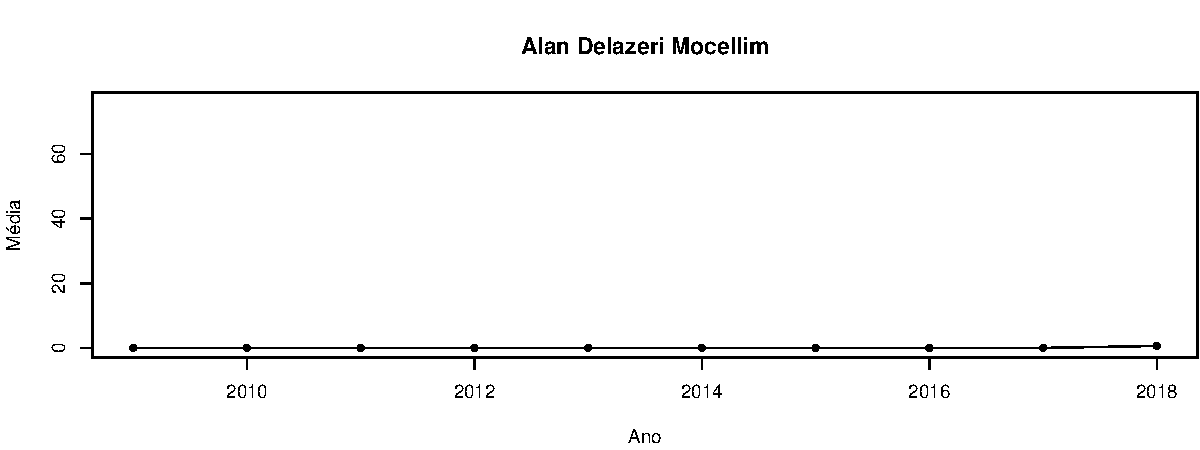
\includegraphics[width=\maxwidth]{figure/mediamovel-1} 

}



\vspace{0.5cm}


{\centering 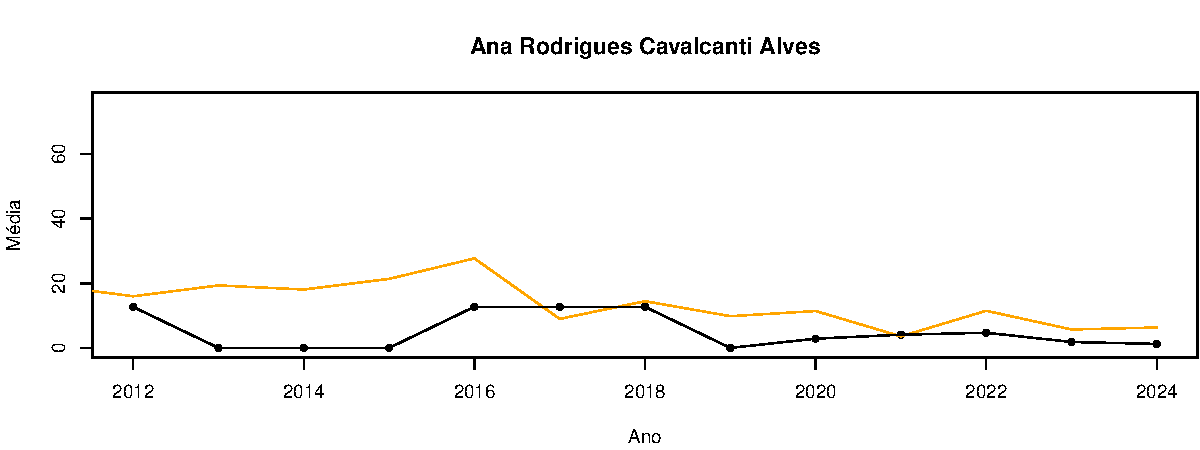
\includegraphics[width=\maxwidth]{figure/mediamovel-2} 

}



\vspace{0.5cm}


{\centering 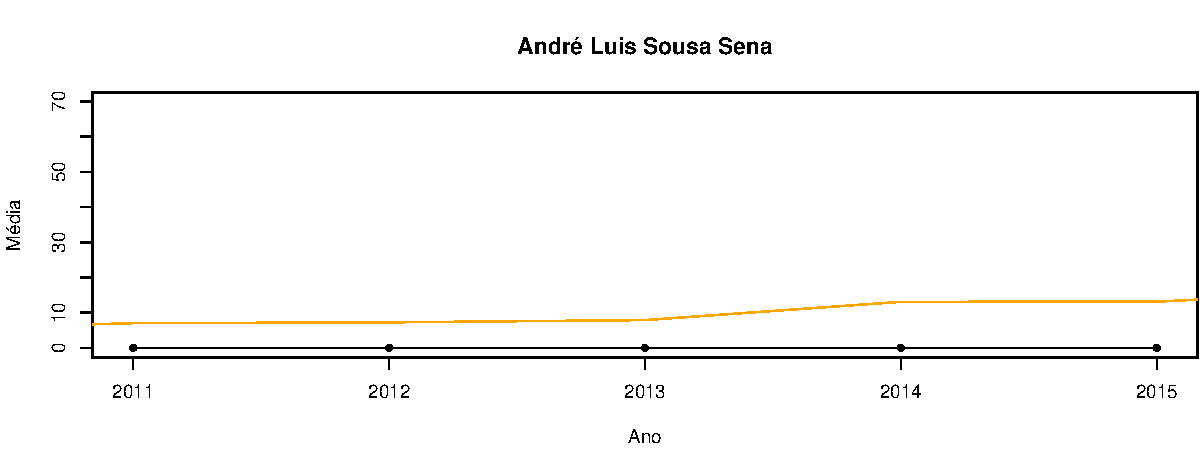
\includegraphics[width=\maxwidth]{figure/mediamovel-3} 

}



\vspace{0.5cm}


{\centering 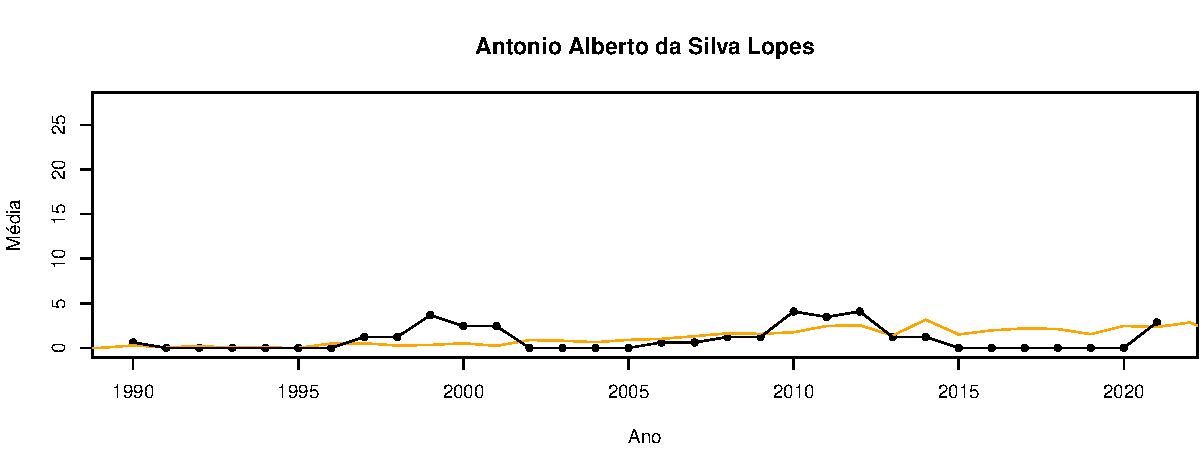
\includegraphics[width=\maxwidth]{figure/mediamovel-4} 

}



\vspace{0.5cm}


{\centering 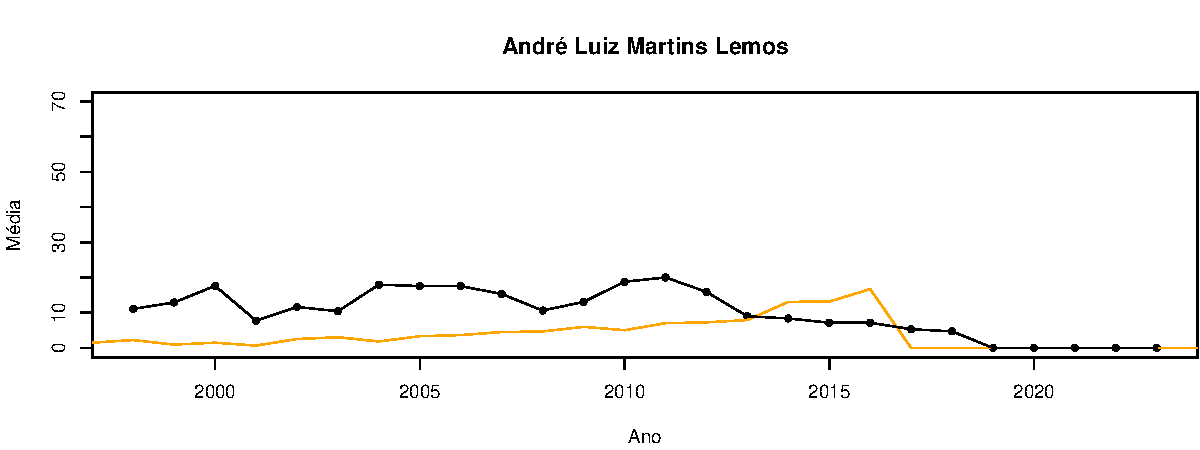
\includegraphics[width=\maxwidth]{figure/mediamovel-5} 

}



\vspace{0.5cm}


{\centering 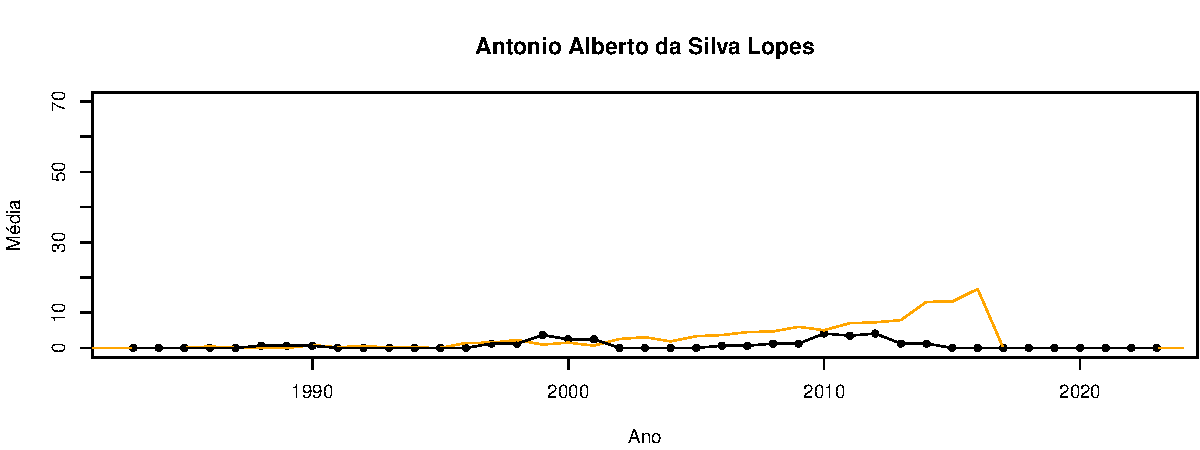
\includegraphics[width=\maxwidth]{figure/mediamovel-6} 

}



\vspace{0.5cm}


{\centering 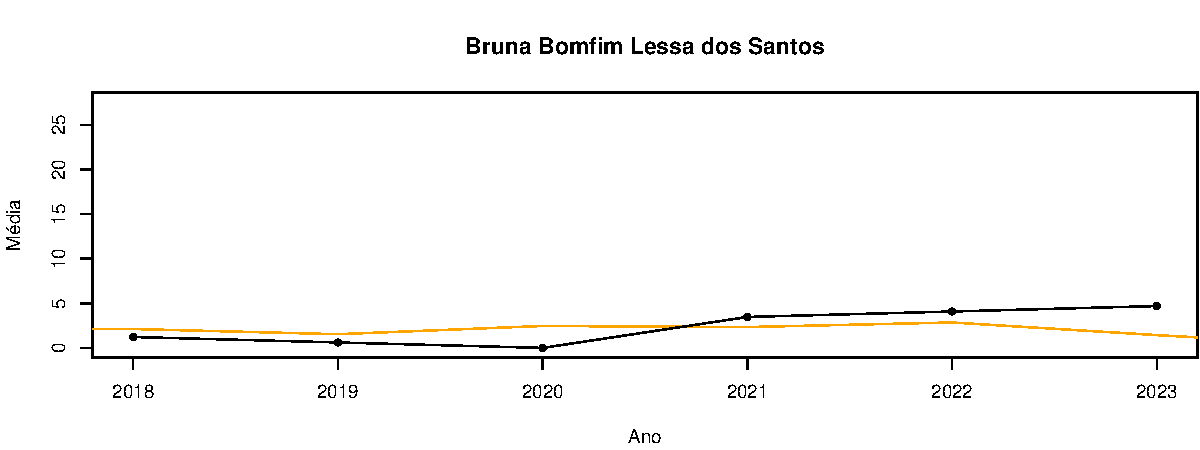
\includegraphics[width=\maxwidth]{figure/mediamovel-7} 

}



\vspace{0.5cm}


{\centering 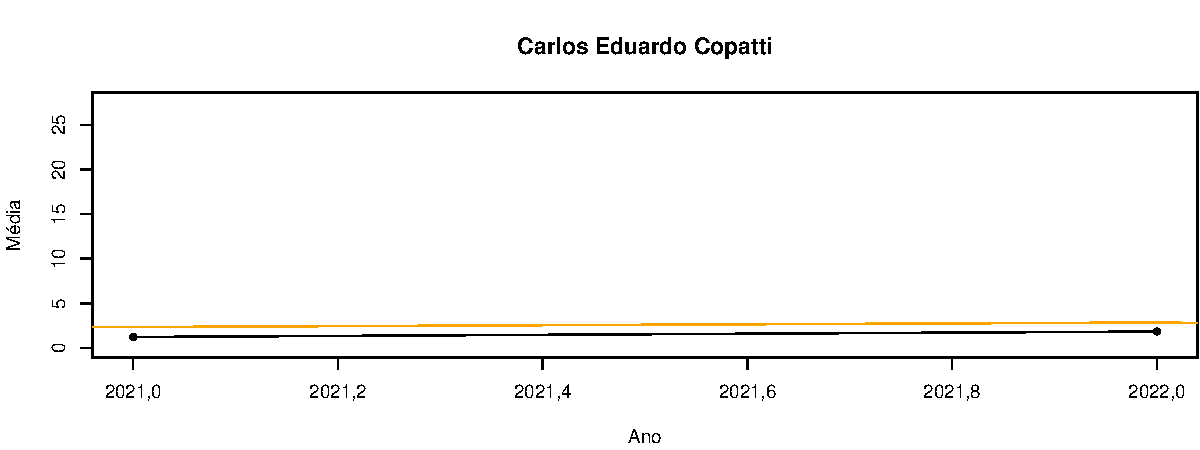
\includegraphics[width=\maxwidth]{figure/mediamovel-8} 

}



\vspace{0.5cm}


{\centering 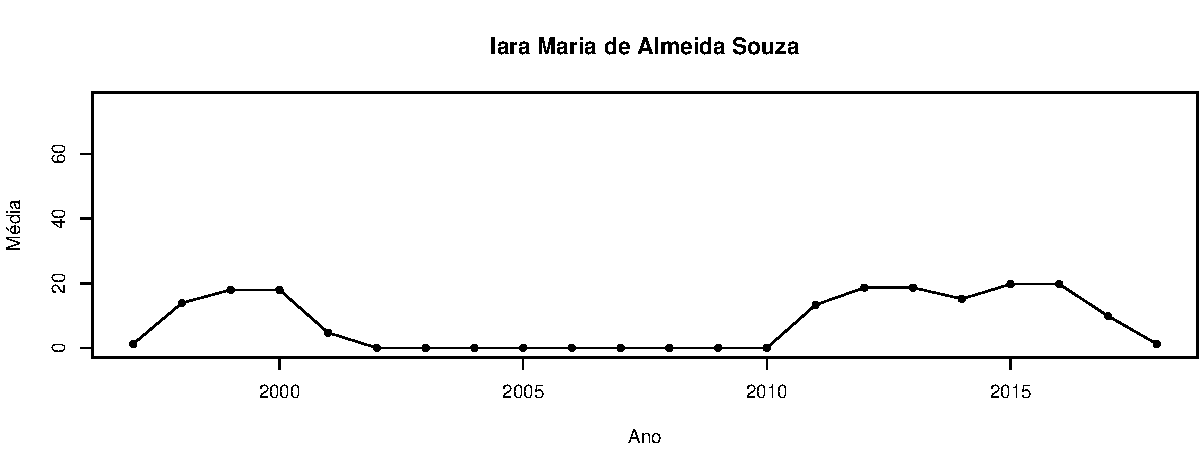
\includegraphics[width=\maxwidth]{figure/mediamovel-9} 

}



\vspace{0.5cm}


{\centering 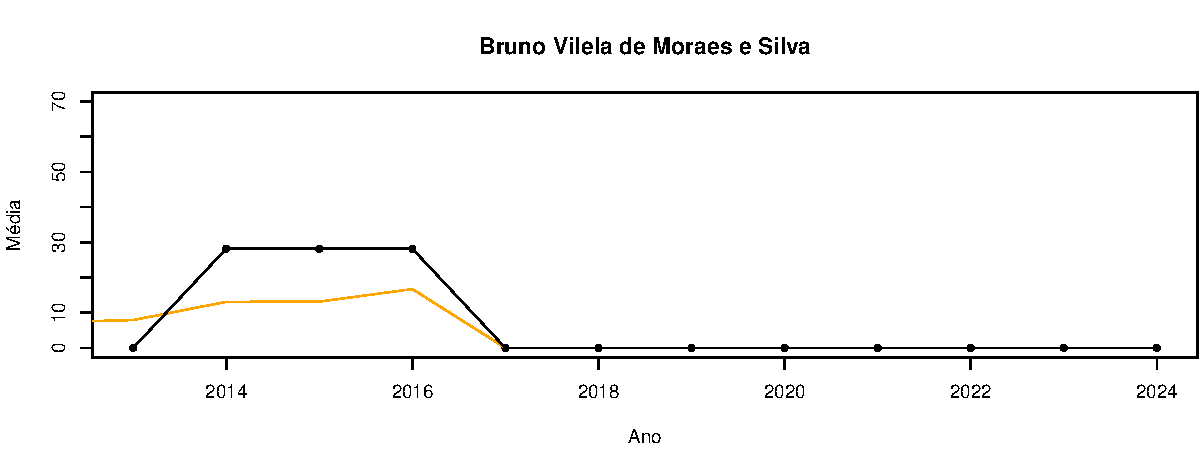
\includegraphics[width=\maxwidth]{figure/mediamovel-10} 

}



\vspace{0.5cm}


{\centering 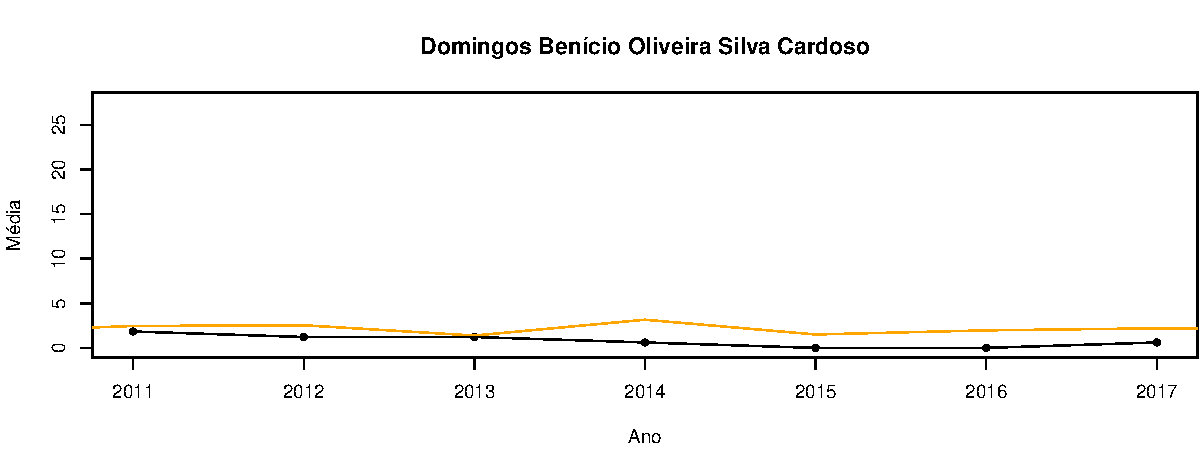
\includegraphics[width=\maxwidth]{figure/mediamovel-11} 

}



\vspace{0.5cm}


{\centering 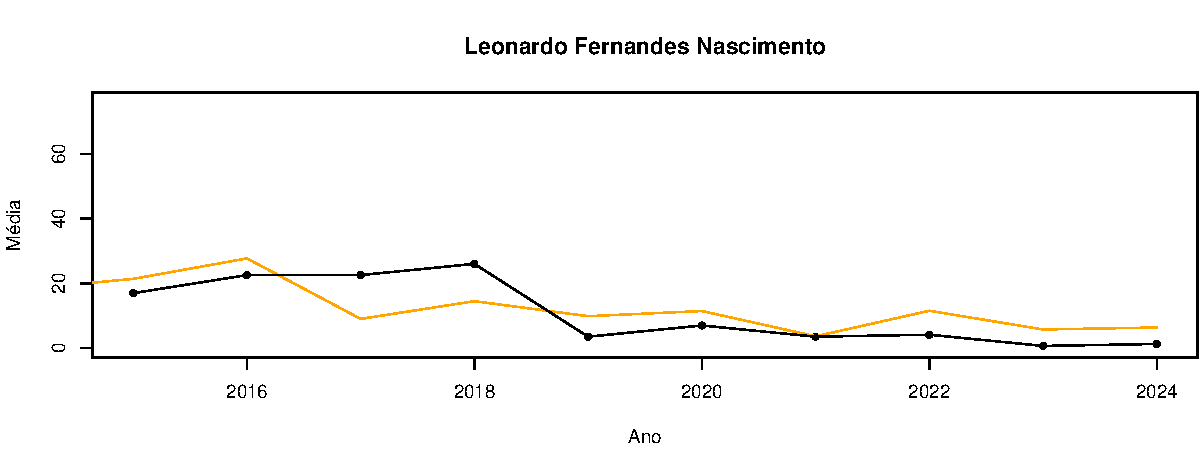
\includegraphics[width=\maxwidth]{figure/mediamovel-12} 

}



\vspace{0.5cm}


{\centering 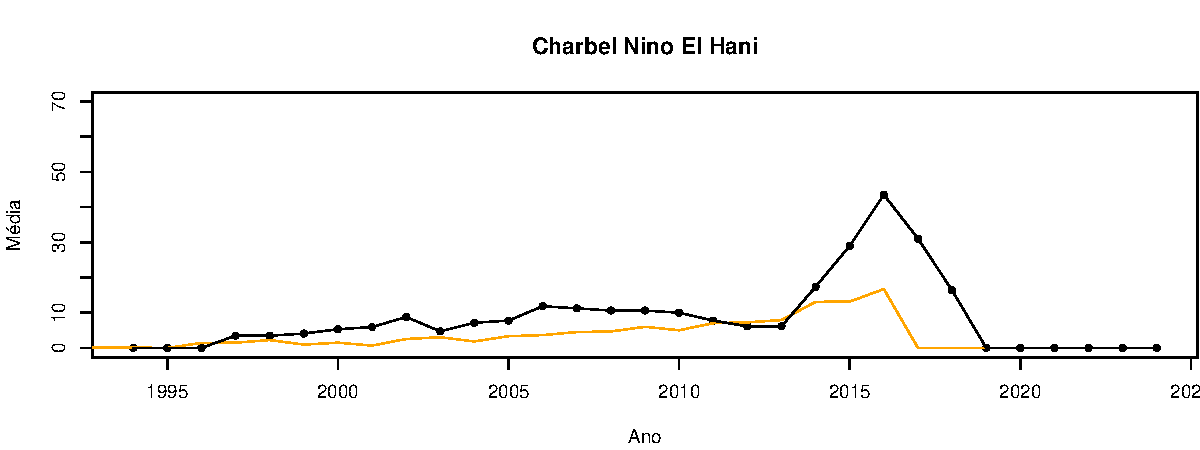
\includegraphics[width=\maxwidth]{figure/mediamovel-13} 

}



\vspace{0.5cm}


{\centering 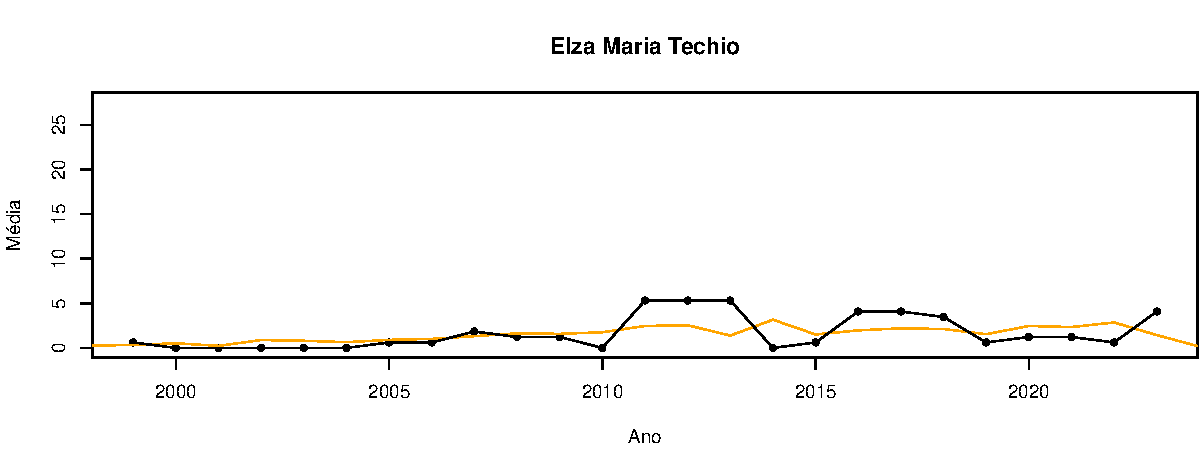
\includegraphics[width=\maxwidth]{figure/mediamovel-14} 

}



\vspace{0.5cm}


{\centering 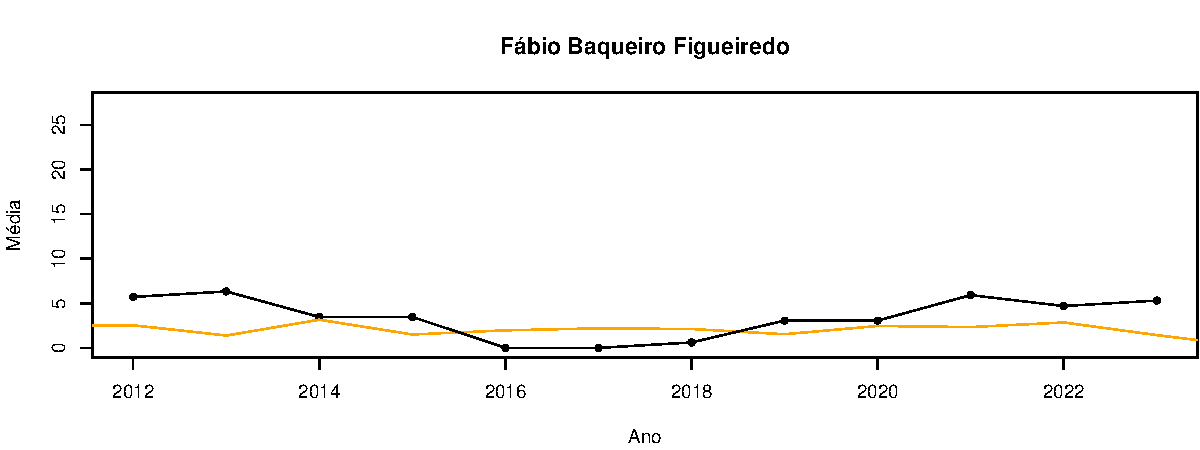
\includegraphics[width=\maxwidth]{figure/mediamovel-15} 

}



\vspace{0.5cm}


{\centering 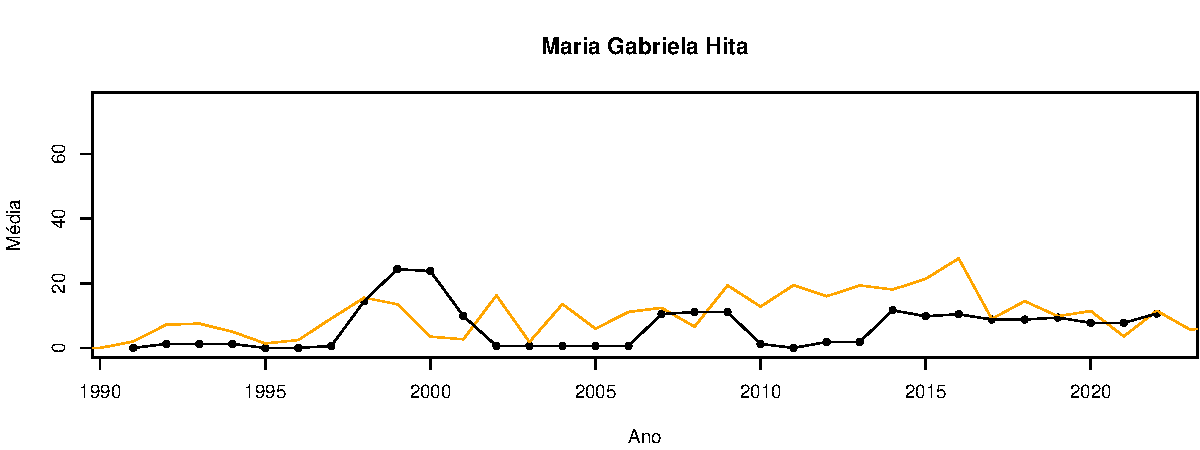
\includegraphics[width=\maxwidth]{figure/mediamovel-16} 

}



\vspace{0.5cm}


{\centering 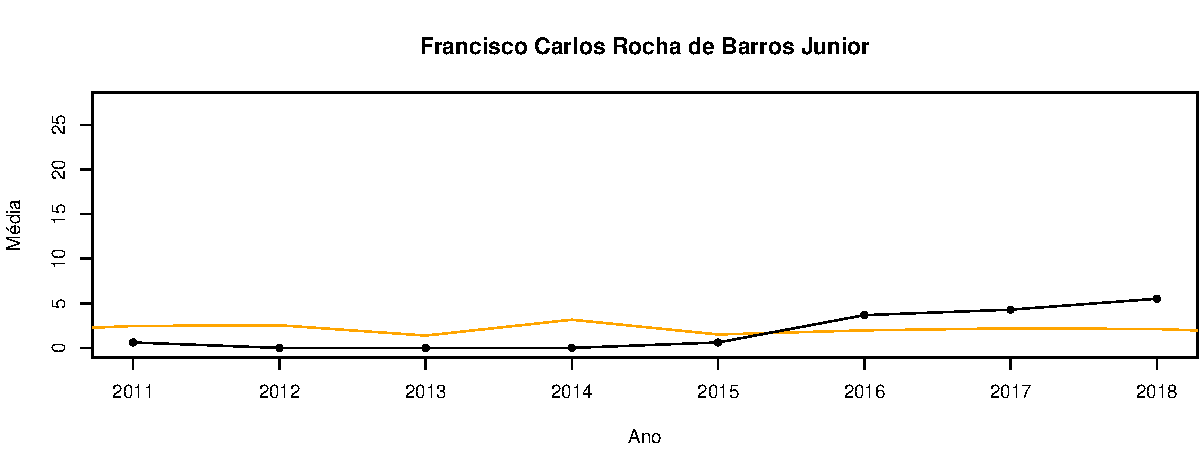
\includegraphics[width=\maxwidth]{figure/mediamovel-17} 

}



\vspace{0.5cm}


{\centering 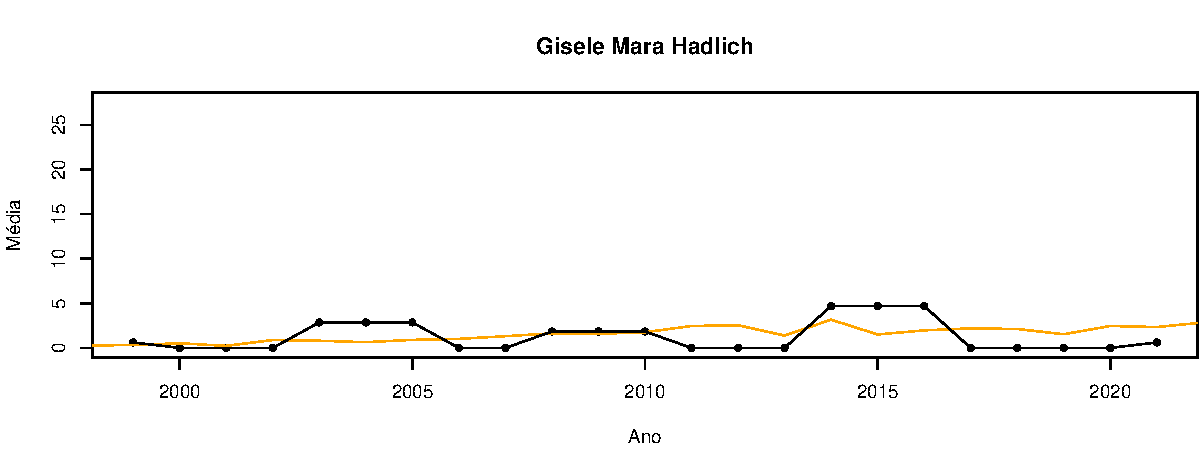
\includegraphics[width=\maxwidth]{figure/mediamovel-18} 

}



\vspace{0.5cm}


{\centering 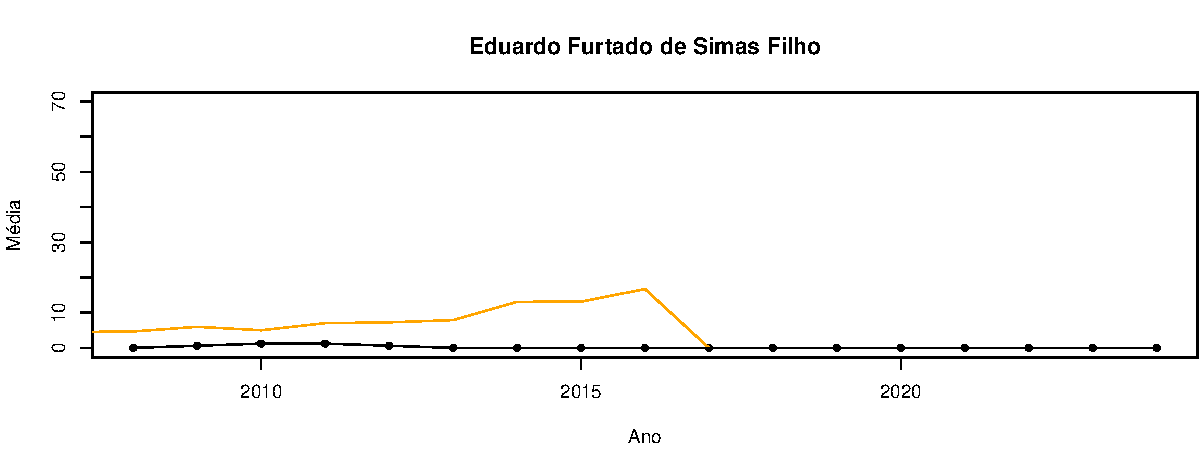
\includegraphics[width=\maxwidth]{figure/mediamovel-19} 

}



\vspace{0.5cm}


{\centering 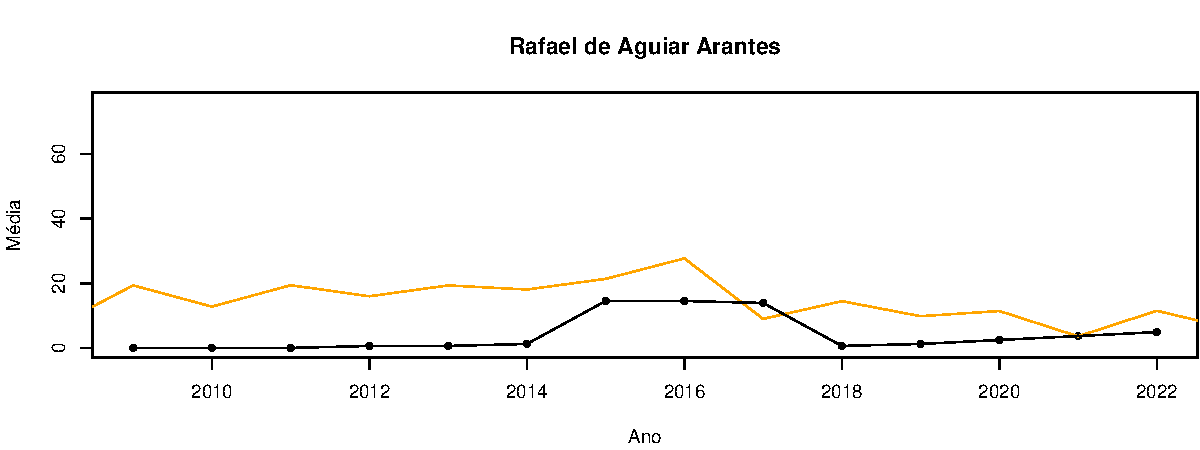
\includegraphics[width=\maxwidth]{figure/mediamovel-20} 

}



\vspace{0.5cm}


{\centering 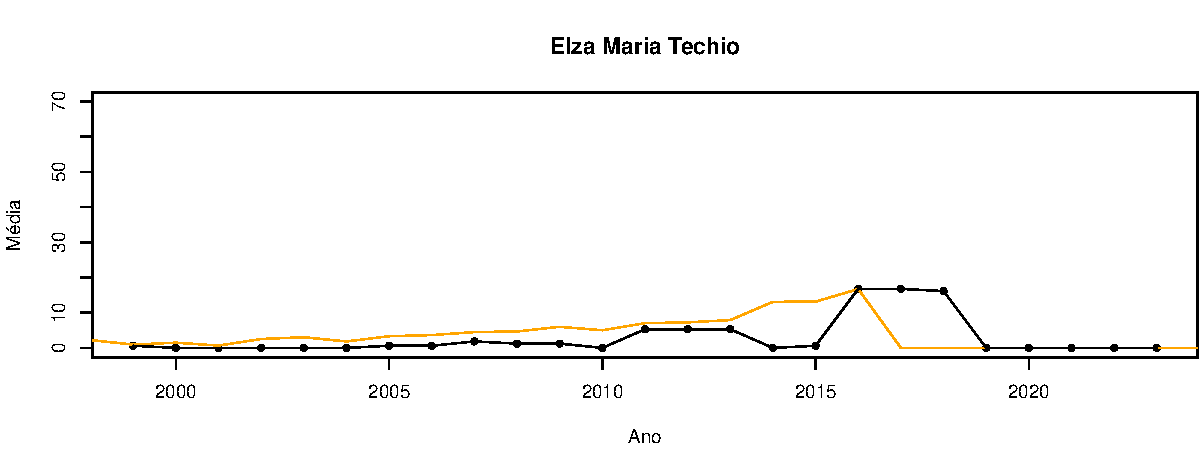
\includegraphics[width=\maxwidth]{figure/mediamovel-21} 

}



\vspace{0.5cm}


{\centering 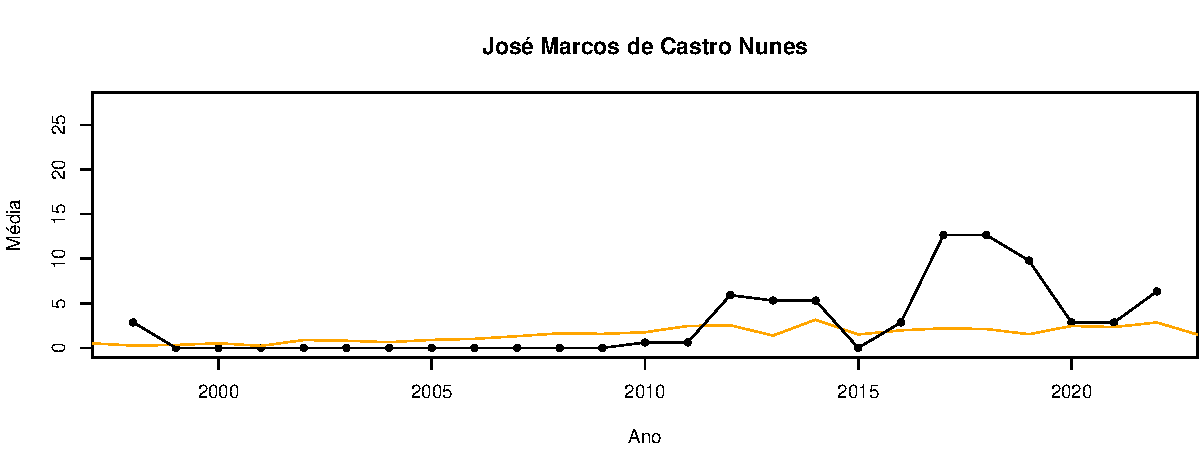
\includegraphics[width=\maxwidth]{figure/mediamovel-22} 

}



\vspace{0.5cm}


\clearpage

\section{Apêndices}

A tabela seguinte lista a produção com coautoria entre professores do
programa e, nas três últimas colunas, mostra o número de autores, sendo a
coautoria identificada de acordo com três métodos:

\vspace{2mm}

\begin{tabular}{crl}
 ~~~~~~~~~ &  \textbf{N} & Nome completo dos autores.\\
 ~~~~~~~~~ &  \textbf{C} & Código do CNPq dos autores.\\
 ~~~~~~~~~ &  \textbf{V} & Coincidência de ISSN/ISBN, ano, tipo de produção (livro, artigo ou capítulo), volume, número e página inicial. \\
\end{tabular}

\phantomsection\stepcounter{tabela}\addcontentsline{lot}{table}{Tabela \thetabela: Trabalhos produzidos em coautoria}
\begin{longtable}{|E{3cm}|E{6cm}|c|E{5cm}|r|r|r|r|}
    \multicolumn{8}{c}{\textbf{Tabela \thetabela: Trabalhos produzidos em coautoria}} \\
    \hline
    \multirow{2}{*}{\textbf{Professor}} & \multirow{2}{*}{\textbf{Produção}} &
    \multirow{2}{*}{\textbf{Ano}} & \multirow{2}{*}{\textbf{Livro ou periódico}} &
    \multirow{2}{*}{\textbf{ISSN ou ISBN}} & \multicolumn{3}{c|}{\textbf{N. Aut.}} \\
    \cline{6-8} & & & & & \textbf{N} & \textbf{C} & \textbf{V} \\
    \hline
    \endfirsthead
    \multicolumn{8}{c}{{\footnotesize ... continuação da página anterior}} \\
    \hline
    \multirow{2}{*}{\textbf{Professor}} & \multirow{2}{*}{\textbf{Produção}} &
    \multirow{2}{*}{\textbf{Ano}} & \multirow{2}{*}{\textbf{Livro ou periódico}} &
    \multirow{2}{*}{\textbf{ISSN ou ISBN}} & \multicolumn{3}{c|}{\textbf{N. Aut.}} \\
    \cline{6-8} & & & & & \textbf{N} & \textbf{C} & \textbf{V} \\
    \endhead
    \hline
    \multicolumn{8}{r}{{\footnotesize Continua na próxima página}} \\
    \endfoot
    \hline
    \endlastfoot
\begin{kframe}


{\ttfamily\noindent\bfseries\color{errorcolor}{\#\# Error in eval(expr, envir, enclos): objeto 'coaut' não encontrado}}\end{kframe}
\end{longtable}

\clearpage

\textbf{Legenda de informação adicional indicada na tabela seguinte}:

\begin{tabular}{E{23.5cm}}
\rowcolor{coautr}Produção realizada em coautoria por mais de um professor do programa.\\
\end{tabular}


\textbf{Legenda de erros de preenchimento do Lattes indicados na tabela seguinte}:

\begin{tabular}{E{23.5cm}}
\rowcolor{capdup}Capítulo indevidamente registrado porque pertence a livro do próprio professor.\\
\rowcolor{ninval}O ISBN é inválido. Confira se todos os algarismos estão corretos.\\
\rowcolor{duplic}Produção registrada mais de uma vez.\\
\end{tabular}


\small
\label{tab:proddet}
\phantomsection\stepcounter{tabela}\addcontentsline{lot}{table}{Tabela \thetabela: Produção detalhada}
\label{ tab:proddet }
\begin{longtable}{lllrrllrr}
\multicolumn{8}{c}{\textbf{Tabela \thetabela: Produção detalhada}} \\
  \toprule
\textbf{Professor} & \textbf{Produção (títulos truncados)} & \textbf{Ano} & \textbf{Qualis} & \textbf{SJR} & \textbf{SNIP} & \textbf{Periódico ou Livro (títulos truncados)} & \textbf{ISSN/ISBN} \\
\midrule
\endfirsthead
\multicolumn{8}{c}{{\footnotesize ... continuação da página anterior}} \\
  \toprule
\textbf{Professor} & \textbf{Produção (títulos truncados)} & \textbf{Ano} & \textbf{Qualis} & \textbf{SJR} & \textbf{SNIP} & \textbf{Periódico ou Livro (títulos truncados)} & \textbf{ISSN/ISBN} \\
\midrule
\endhead
\midrule
\multicolumn{8}{r}{{\footnotesize Continua na próxima página}} \\
\endfoot
\bottomrule
\endlastfoot
Alan Mocellim & A cibercultura para além das dic & 2010 & SQ &  &  & Socitec E-prints & 18088333 \\
Alan Mocellim & A comunidade: da sociologia clás & 2010 & SQ &  &  & PLURAL (USP) & 01046721 \\
Alan Mocellim & A dinâmica social no Orkut & 2010 & SQ &  &  & Cientec: Revista de Ciência, Tecnolo & 19849710 \\
Alan Mocellim & Comunicação e Reencantamento: re & 2015 & SQ &  &  & ESFERAS & 24466190 \\
Alan Mocellim & O reencantamento científico do m & 2015 & SQ &  &  & REVISTA BRASILEIRA DE SOCIO & 23180544 \\
Alan Mocellim & Zygmunt Bauman & 2018 & Cap &  &  & Os sociólogos: de Auguste Comte a Gi & 8532659470 \\
Ana Alves & O conceito de hegemonia: de Gram & 2010 & A2 & 0,189 & 0,377 & Lua Nova. Revista de Cultura e Polít & 01026445 \\
Ana Alves & A nova abordagem racial da telen & 2012 & B2 &  &  & ESTUDOS DE SOCIOLOGIA (RECI & 1415000X \\
Ana Alves & A (des) continuidade da Tradição & 2016 & Lvr &  &  &  & 9788541508667 \\
Ana Alves & Dos habitus de classe aos patrim & 2016 & B1 &  &  & Sociologias (UFRGS) & 18070337 \\
Ana Alves & Com o suor do trabalho: uma anál & 2020 & Lvr &  &  &  & 9786586732917 \\
Antonio Camara & A DÍADE SUBJETIVIDADE/OBJET & 2010 & SQ &  &  & Crítica \& Debates: Revista de Histó & 21789827 \\
Antonio Camara & Representação fílmica da favela  & 2011 & C &  &  & Cadernos de Estudos Sociais & 01024248 \\
Antonio Camara & Uma re-leitura de Kant: crítica  & 2012 & SQ &  &  & Contra a Corrente: Revista Marxista  & 19845898 \\
Antonio Camara & A representação do conflito nos  & 2013 & SQ &  &  & Revista Prelúdio & 23187808 \\
Antonio Camara & A subjetividade/objetividade na  & 2013 & Cap &  &  & Cinema Documentário Brasileiro em Pe & 9788523210984 \\
Antonio Camara & Cinema Documentário Brasileiro e & 2013 & Org &  &  &  & 9788523210984 \\
Antonio Camara & Da estética à sociologia da arte & 2013 & Cap &  &  & Cinema Documentário Brasileiro em Pe & 9788523210984 \\
Antonio Camara & Imagens da exclusão Social & 2013 & Cap &  &  & Cinema Documentário Brasileiro em Pe & 9788523210984 \\
Antonio Camara & Marx: Razão, sensibilidade, eman & 2013 & SQ &  &  & Contra a Corrente: Revista Marxista  & 19845898 \\
Antonio Camara & Sobre modo de vida e arte em Tro & 2013 & SQ &  &  & CONTRA A CORRENTE: REVISTA  & 19845898 \\
Antonio Camara & Zumbi somos nós e Frente 3 de Fe & 2013 & Cap &  &  & Cinema Documentário Brasileiro em Pe & 9788523210984 \\
Antonio Camara & Neo.realismo italiano: desespero & 2014 & SQ &  &  & CONTRA A CORRENTE: REVISTA  & 19845898 \\
Antonio Camara & Limites do Desenvolvimento Suste & 2015 & Cap &  &  & Dialógo em Transito: Brasil, Cabo Ve & 9788523213923 \\
Antonio Camara & Apresentação & 2016 & Cap &  &  & Estudos socioambientais e saberes tr & 9788523215255 \\
Antonio Camara & Estudos socioambientais e sabere & 2016 & Org &  &  &  & 9788523215255 \\
Antonio Camara & I Encontro Arte e Sociedade & 2016 & Org &  &  &  & 9788582920923 \\
Antonio Camara & Litoral Norte em Imagens & 2016 & Cap &  &  & Estudos socioambientais e saberes tr & 9788523215255 \\
Antonio Camara & Turismo e meio ambiente em Sauíp & 2016 & Cap &  &  & Estudos socioambientais e saberes tr & 9788523215255 \\
Antonio Camara & Abordagens sobre a sociologia da & 2018 & Cap &  &  & Ensaios arte e sociedade & 9788523217846 \\
Antonio Camara & Contribuição para uma sociologia & 2018 & Cap &  &  & Ensaios de Sociologia da arte & 9788523217846 \\
Antonio Camara & Ensaios de Sociologia da Arte & 2018 & Org &  &  &  & 9788523217846 \\
Antonio Camara & Pressupostos filosóficos clássic & 2018 & Cap &  &  & Ensaios de Sociologia da Arte & 9788523217846 \\
Antonio Camara & Reflexões para uma sociologia da & 2018 & Cap &  &  & Ensaios de sociologia da arte & 9788523217846 \\
Antonio Camara & ENJEUX ENVIRONNEMENTAUX ET  & 2019 & Org &  &  &  & 9782343180199 \\
Antonio Camara & INTRODUÇÃO & 2019 & Cap &  &  & ENJEUX ENVIRONNEMENTAUX ET  & 9782343180199 \\
Antonio Camara & LE LITTORAL NORD EM IMAGES & 2019 & Cap &  &  & ENJEUX ENVORONNEMENTAUX ET  & 9782343180199 \\
Clóvis Zimmermann & As Políticas sociais e os Direit & 2010 & Cap &  &  & DESIGUALDADES E JUSTIÇA SOC & 9788598885964 \\
Clóvis Zimmermann & O CURSO DE GESTÃO PÚBLICA N & 2010 & B4 &  &  & Temas de administração pública (UNES & 19824637 \\
Clóvis Zimmermann & O Princípio Democrático e Consti & 2010 & B3 &  &  & Revista Internacional de Direito e C & 19831811 \\
Clóvis Zimmermann & A institucionalização da assistê & 2011 & SQ &  &  & Acta Scientiarum. Human and Social S & 16797361 \\
Clóvis Zimmermann & As tipologias de Estado de bem-e & 2011 & Cap &  &  & Políticas Públicas em Foco: Concepçõ & 9788561346188 \\
Clóvis Zimmermann & Combate à pobreza e miséria  no  & 2011 & Cap &  &  & DIREITO HUMANO  À ALIMENTAÇ & 9788599184851 \\
Clóvis Zimmermann & Das Grundeinkommen im Rahmen der & 2011 & Cap &  &  & Soziale Sicherheit in Lateinamerika & 9783865736376 \\
Clóvis Zimmermann & Noch zu wenig linke Akzente: Ers & 2011 & B2 &  &  & Lateinamerika-Nachrichten & 01746324 \\
Clóvis Zimmermann & The incomplete revolution & 2011 & B1 &  & 0,267 & Cadernos CRH & 01034979 \\
Clóvis Zimmermann & Combate à fome e miséria no gove & 2012 & C &  &  & Revista Espaço Acadêmico (UEM) & 15196186 \\
Clóvis Zimmermann & Noch kein neuer Sozialvertrag & 2012 & B4 &  &  & Brasilien-Nachrichten & 01736582 \\
Clóvis Zimmermann & Noch kein neuer Sozialvertrag: T & 2012 & B2 &  &  & Lateinamerika-Nachrichten & 01746324 \\
Clóvis Zimmermann & Plano Brasil Sem Miséria e o dir & 2012 & Cap &  &  & Direito Humano à Alimentação Adequad & 9788599184 \\
Clóvis Zimmermann & As políticas sociais sob o signo & 2015 & SQ &  &  & Conjuntura \& Planejamento & 14131536 \\
Clóvis Zimmermann & Impacto dos programas de transfe & 2015 & Cap &  &  & Diálogos em trânsito:Brasil, Cabo Ve & 9788523213923 \\
Clóvis Zimmermann & Metodologia e Epistemologia das  & 2015 & Org &  &  &  & 9788562756429 \\
Clóvis Zimmermann & PARA ALÉM DE QUESTÕES ELEIT & 2015 & Cap &  &  & \#DEMOCRACIABR: O MOMENTO P & 9788562756474 \\
Clóvis Zimmermann & Programas sociais no Brasil: um  & 2015 & A2 &  & 0,267 & Cadernos CRH (Online) & 19838239 \\
Clóvis Zimmermann & Direitos Humanos na Democracia C & 2018 & Org &  &  &  & 9788570770011 \\
Clóvis Zimmermann & Políticas sociais na perspectiva & 2018 & Cap &  &  & ?Direitos Humanos na Democracia Cont & 9788570770011 \\
\rowcolor{ninval}Clóvis Zimmermann & Estado, proteção social e segura & 2019 & Lvr &  &  &  & 9788523218389 \\
Clóvis Zimmermann & Reformas no Estado de Bem-Estar  & 2019 & Cap &  &  & Estado, proteção social e segurança  & 9788523218379 \\
Débora Previatti & Determinação social do processo  & 2012 & Cap &  &  & As bases da dispensação racional de  & 8589731561 \\
Débora Previatti & Em busca da interdisciplinaridad & 2013 & Cap &  &  & Contribuições para a Gestão do SUS & 9788578400842 \\
Débora Previatti & Profissões de saúde: socializaçã & 2015 & Cap &  &  & Leituras do mundo do trabalho: um ol & 9788568267165 \\
Débora Previatti & Práticas, fluxos e símbolos na A & 2016 & Lvr &  &  &  & 9788579614958 \\
Eduardo Machado & Os bancários não vão ao paraiso: & 2010 & Cap &  &  & Violência e Conflitos Sociais: traje & 9788571133 \\
Eduardo Machado & Polícia para quem precisa de pol & 2010 & B1 &  & 0,267 & Cadernos CRH & 01034979 \\
Eduardo Machado & Policiamento e polícia & 2010 & Org &  & 0,267 &  & 01034979 \\
Eduardo Machado & The deliveries cannot stop: ecol & 2010 & SQ & 0,437 & 1,162 & Crime, Law and Social Change (Print) & 09254994 \\
Eduardo Machado & Bank employees don’t go to Heave & 2011 & Cap &  &  & Psychology of Victimization & 9781614705055 \\
Eduardo Machado & Motoboys, atividade arriscada e  & 2011 & Cap &  &  & Violência e dilemas civilizatórios:  & 9788571133914 \\
Eduardo Machado & Governança multicêntrica e redes & 2012 & B5 & 0,211 & 0,977 & Dilemas: Revista de Estudos de Confl & 19835922 \\
Eduardo Machado & Conducting danger: practices and & 2013 & SQ & 0,394 & 0,859 & International Journal of Comparative & 01924036 \\
Eduardo Machado & Processos sociais de vitimização & 2013 & B1 & 0,541 & 1,051 & Tempo Social (USP. Impresso) & 01032070 \\
Eduardo Machado & Segurança pública: polícia, demo & 2013 & B3 &  &  & Espacio Abierto (Caracas. 1992) & 13150006 \\
Eduardo Machado & Conduzindo o perigo: governança, & 2014 & Cap &  &  & Violência, ilegalismos e lugares mor & 9788571135796 \\
Eduardo Machado & Conduzindo o perigo: práticas e  & 2014 & B3 &  &  & Espacio Abierto (Caracas. 1992) & 13150006 \\
Eduardo Machado & No place to run, no place to hid & 2014 & SQ & 0,527 & 1,076 & Australian and New Zealand Journal o & 00048658 \\
Eduardo Machado & O lado sombrio da estrada vitimi & 2015 & A2 &  & 0,276 & Revista Brasileira de Ciências Socia & 18069053 \\
Eduardo Machado & Governing security in the street & 2016 & Cap &  &  & Crime and criminal behavior & 9781634855808 \\
Eduardo Machado & Introduction & 2016 & SQ &  & 1,169 & Police Practice and Research & 1477271X \\
Eduardo Machado & Percepção de medo e gestão de ví & 2016 & Cap &  &  & Violência, territorialidades e negoc & 9788571137943 \\
Eduardo Machado & Policing drug markets & 2016 & Org & 0,576 & 1,169 &  & 15614263 \\
Eduardo Machado & Sem lugar para correr, nem se es & 2016 & Cap &  &  & Paradoxos da segurança cidadã & 9788586225963 \\
Eduardo Machado & Vulnerabilidade no ambiente de t & 2017 & Cap &  &  & Escolas em tempo de crise: estudos e & 9788523216528 \\
Eduardo Machado & Governança da segurança como uma & 2020 & Cap &  &  & Meandros da atenção e gestão no enfr & 9786587115047 \\
Elisio Estanque & Juventude, boemia e movimentos s & 2010 & SQ &  &  & Revista Política e Sociedade & 21757984 \\
Elisio Estanque & Sindicalismo e movimentos sociai & 2010 & B3 &  &  & LUTAS SOCIAIS (PUCSP) & 1415854X \\
Elisio Estanque & Cultura estudantil, ?Republicas? & 2011 & Cap &  &  & Jovens e Rumos & 9789726712855 \\
Elisio Estanque & Informalidades, precariedades e  & 2011 & Cap &  &  & Marchas e contramarchas da informali & 8577458350 \\
Elisio Estanque & O Sindicalismo Português e a Nov & 2011 & Lvr &  &  &  & 9789724044989 \\
Elisio Estanque & Os sujeitos que nunca foram hist & 2011 & B3 &  &  & INTERTHESIS (FLORIANÓPOLIS) & 18071384 \\
Elisio Estanque & Sociedade e trabalho no contexto & 2011 & Cap &  &  & Integraçao Europeia e Processos de T & 9789661905121 \\
Elisio Estanque & A Classe Média. Ascensão e Declí & 2012 & Lvr &  &  &  & 9789898424464 \\
Elisio Estanque & Labour relations and social move & 2012 & Cap &  &  & Sociological Landscapes: Theories, R & 9799533075111 \\
Elisio Estanque & Le Portugal en piètre état & 2012 & SQ &  &  & Relations (Montréal) & 00343781 \\
Elisio Estanque & O Estado Social em Causa: instit & 2012 & Cap &  &  & Finisterra ? Revista de Reflexão e C & 9787387179826 \\
Elisio Estanque & Precariedade, sindicalismo e açã & 2012 & SQ &  &  & Revista Configurações & 21827419 \\
Elisio Estanque & Trabalho, classe média e sindica & 2012 & Cap &  &  & Facetas do Trabalho na Contemporanei & 9788581920986 \\
Elisio Estanque & Trabalho, Juventude e Precarieda & 2012 & Org &  &  &  & 9788579172021 \\
Elisio Estanque & Trabalho, precariedade e movimen & 2012 & Cap &  &  & Trabalho, Juventude e Precariedade & 9788579172021 \\
Elisio Estanque & Transformação social, democracia & 2012 & SQ &  &  & Revista da FAE & 15161234 \\
Elisio Estanque & A ?classe média? como realidade  & 2013 & Cap &  &  & A ?Nova Classe Média? no Brasil como & 9788562669101 \\
Elisio Estanque & Crise, Estado social e desafios  & 2013 & B1 &  &  & Educar em Revista (Impresso) & 01044060 \\
Elisio Estanque & Facetas do trabalho na Contempor & 2013 & Org &  &  &  & 9788581920986 \\
Elisio Estanque & O desemprego é uma oportunidade? & 2013 & Cap &  &  & Não Acredite em Tudo o Que Pensa & 9789896711573 \\
Elisio Estanque & O Estado Social em Causa: instit & 2013 & SQ & 0,240 & 0,562 & FINISTERRA (LISBOA. 1966) & 04305027 \\
\rowcolor{duplic}Elisio Estanque & O Estado social em causa: Instit & 2013 & Cap &  &  & Os Portugueses e o Estado-Providênci & 9789726713203 \\
Elisio Estanque & O sindicalismo europeu no centro & 2013 & SQ &  & 0,274 & JANUS.NET, e-journal of Int & 16477251 \\
Elisio Estanque & The new global cycle of protest  & 2013 & SQ & 0,370 & 0,757 & Journal of Social Science Education & 16185293 \\
Elisio Estanque & Trabalho e sindicalismo: crise,  & 2013 & Cap &  &  & Riqueza e miséria do trabalho no Bra & 9788575593264 \\
Elisio Estanque & Trabalho, inovação e coesão soci & 2013 & Cap &  &  & 25 anos de Portugal europeu: Comentá & 9789898662224 \\
\rowcolor{duplic}Elisio Estanque & Trabalho, precariedade e movimen & 2013 & Cap &  &  & Mudanças Laborais e Relações de Géne & 9789724048079 \\
Elisio Estanque & A metodologia de observação part & 2014 & Cap &  &  & Metodologia de Investigação em Ciênc & 9789897550508 \\
Elisio Estanque & Dinâmicas de classe média e rebe & 2014 & SQ &  &  & EMANCIPAÇÃO (ONLINE) (PONTA & 19827814 \\
Elisio Estanque & O despotismo fabril: violência e & 2014 & Cap &  &  & Pesquisa e Extensão. Experiências e  & 9788577981915 \\
Elisio Estanque & Olas de Indignación y su Lógica  & 2014 & SQ &  &  & Revista de la Asociación de Sociolog & 19887302 \\
Elisio Estanque & Rebeliões de classe média? Preca & 2014 & B2 &  & 0,352 & Revista Crítica de Ciências Sociais & 02541106 \\
Elisio Estanque & Trabalho, precariedade e rebeliõ & 2014 & B2 &  & 0,352 & Revista Crítica de Ciências Sociais & 21827435 \\
Elisio Estanque & Trabalho, precariedade e rebeliõ & 2014 & Org &  & 0,352 &  & 21827435 \\
Elisio Estanque & Classe Média e Lutas Sociais: en & 2015 & Lvr &  &  &  & 9788526812727 \\
Elisio Estanque & Discurso, Trabalho e Movimentos  & 2015 & Lvr &  &  &  & 9788579932533 \\
Elisio Estanque & Middle-class Rebellions? Precari & 2015 & SQ &  &  & RCCS ANNUAL REVIEW & 16473175 \\
Elisio Estanque & O futuro do sindicalismo na repr & 2015 & Cap &  &  & O Futuro dos Sistemas de Representaç & 9789897500381 \\
Elisio Estanque & As lutas da classe média & 2016 & Cap &  &  & Sociologia e Sociedade: estudos de h & 9789898536549 \\
Elisio Estanque & Onde pára a classe média? Breves & 2016 & SQ &  &  & SOCIOLOGIA, PROBLEMAS E PRÁ & 21827907 \\
Elisio Estanque & Praxe e Tradições Académicas & 2016 & Lvr &  &  &  & 9789898838452 \\
Elisio Estanque & A classe média à deriva & 2017 & Cap &  &  & Espaços e Tempos em Geografia. Livro & 9789892613482 \\
\rowcolor{duplic}Elisio Estanque & A classe média à deriva & 2018 & Cap &  &  & Espaços e Tempos em Geografia. Livro & 9892613481 \\
Elisio Estanque & Building the ?Contraption?: Anti & 2018 & Cap &  &  & Challenging Austerity: Radical Left  & 9781138211 \\
Elisio Estanque & Caloiros e Doutores: um estudo s & 2018 & Lvr &  &  &  & 9789898536662 \\
Elisio Estanque & Die fliegende Kuh« - Warum Recht & 2018 & Cap &  &  & Arbeiterbewegung von rechts? Ungleic & 9783593509716 \\
Elisio Estanque & Social Movements and Organized L & 2018 & Lvr &  &  &  & 9781472472045 \\
Elisio Estanque & Trade Unions and Social Movement & 2018 & Cap &  &  & Social Movements and Organized Labou & 9781472472 \\
Elisio Estanque & Are Trade Unions in Portugal Tra & 2019 & Cap &  &  & Confronting Crisis and Precariousnes & 9781786610478 \\
Elisio Estanque & Desigualdades, tecnologia e revo & 2019 & Cap &  &  & Desigualdades Sociais e Políticas Pú & 9789897553813 \\
Elisio Estanque & Organizações e desafios sociolab & 2019 & Cap &  &  & Economia social - olhares cruzados & 9789724080680 \\
Elisio Estanque & Praxe e tradição estudantil em C & 2019 & Cap &  &  & Os 31 Desafios para o Ensino Superio & 9789895436125 \\
Elisio Estanque & Tempos conturbados no mundo do t & 2019 & Cap &  &  & Negociação Coletiva - Estado e Desaf & 9789897685866 \\
Felipe Vargas & Biotecnologias, risco e direito  & 2011 & C &  &  & Revista de Ciênciais Sociais (UGF) & 14138999 \\
Felipe Vargas & Controvérsias em biotecnologias: & 2012 & Cap &  &  & Contextos rurais e agenda ambiental  & 9788563737038 \\
Felipe Vargas & Por uma coerência nas ciências & 2014 & B3 &  &  & P o l i s e P s i q u e & 2238152X \\
Felipe Vargas & Epistemologia das ciências socia & 2015 & SQ &  &  & Revista Contraponto & 23583541 \\
Felipe Vargas & A história se repete? Controvérs & 2016 & Cap &  &  & Conflitos ambientais e controvérsias & 9788538603092 \\
Felipe Vargas & Controvérsias sobre transgênicos & 2016 & A2 & 0,215 & 0,48 & Novos Estudos. CEBRAP & 01013300 \\
Felipe Vargas & Desenvolvimento sustentável: int & 2016 & Cap &  &  & Introdução às Teorias do Desenvolvim & 9788538603184 \\
Felipe Vargas & Estado, desenvolvimento e neo-de & 2016 & Cap &  &  & Introdução às Teorias do Desenvolvim & 9788538603184 \\
Felipe Vargas & Student Interactive Session: bri & 2016 & Cap &  &  & Inputs form Universidade Federal do  & 9789251093306 \\
Felipe Vargas & Controvérsias em biotecnologias  & 2017 & Lvr &  &  &  & 9783330769588 \\
Felipe Vargas & Ambientes entrelaçados: a conser & 2020 & Cap &  &  & Pesquisa em desenvolvimento, ambient & 9788547345792 \\
Iara Souza & A incrível história da fraude do & 2010 & SQ & 0,355 & 1,103 & História, Ciências, Saúde-Manguinhos & 01045970 \\
Iara Souza & Caderno CRH. Corpos, Lugares e C & 2011 & Org &  &  &  & 0103-4979 \\
Iara Souza & Células-Tronco: considerações so & 2011 & Cap &  &  & Diálogos entre ciência e divulgação  & 9788523207762 \\
\rowcolor{coautr}Iara Souza & Corpos: ações, lugares e coisas  & 2011 & B1 &  & 0,267 & Cadernos CRH & 01034979 \\
Iara Souza & ’Os experimentos que dão errado’ & 2012 & Cap &  &  & Trajetórias, sensibilidades, materia & 9788523210106 \\
Iara Souza & A Paisagem Temporal do Laboratór & 2012 & Cap &  &  & Trajetórias, sensibilidades, materia & 9788523210106 \\
\rowcolor{coautr}Iara Souza & Introdução - Trajetórias, Sensib & 2012 & Cap &  &  & Trajetórias, Sensibilidades e Materi & 9788523210106 \\
Iara Souza & Tecnologia médica em contexto: c & 2012 & Cap &  &  & Informar e educar em saúde: análises & 9788523210427 \\
Iara Souza & Trajetórias, sensibilidades, mat & 2012 & Org &  &  &  & 9788523210106 \\
Iara Souza & Vidas experimentais: humanos e r & 2013 & SQ &  & 0,321 & ETNOGRÁFICA (LISBOA & 08736561 \\
\rowcolor{coautr}Iara Souza & Hermenêutica-fenomenológica e co & 2014 & B1 & 0,310 & 1,215 & Sociedade e Estado (UnB. Impresso) & 01026992 \\
Iara Souza & A importância do espaço para as  & 2015 & SQ &  &  & Revista Latinoamericana de Estudios  & 18528759 \\
Iara Souza & A noção de ontologias múltiplas  & 2015 & SQ &  &  & Ilha - Revista de Antropologia & 21758034 \\
Iara Souza & KOHN, Eduardo. How forests think & 2015 & B1 &  &  & Horizontes Antropológicos (Online) & 18069983 \\
\rowcolor{coautr}Iara Souza & Agência: para além da oposição e & 2018 & Cap &  &  & Políticas etnográficas no campo da c & 9788566094411 \\
Iara Souza & Metodologia e Teoria Ator-Rede & 2018 & Cap &  &  & Novas Fronteiras Metodológicas nas C & 9788523217976 \\
Iracema Guimarães & Gênero e Trabalho: Desafios da I & 2010 & Cap &  &  & Travessias de Gênero na Perspectiva  & 9788588688131 \\
Iracema Guimarães & A Periferia, a casa e a rua: lim & 2011 & Cap &  &  & Gênero, Mulheres e Feminismo & 9788523208516 \\
Iracema Guimarães & Periferias e Territórios sob efe & 2011 & B1 &  & 0,267 & Cadernos CRH & 01034979 \\
Iracema Guimarães & Os idosos em um contexto de trab & 2012 & B3 &  &  & Revista Mediações (UEL) & 14140543 \\
Iracema Guimarães & Resenha do livro‘A cidade nas fr & 2012 & B1 &  & 0,267 & Cadernos CRH & 01034979 \\
Iracema Guimarães & Reprodução e Trabalho & 2013 & Cap &  &  & Dicionário Temático Desenvolvimento  & 9788539105946 \\
Iracema Guimarães & Conseqüencias de uma expansão pe & 2015 & SQ &  &  & 861X ceas revista critica de humanid & 2447861X \\
Iracema Guimarães & Dinâmica Urbana e Contextos de P & 2017 & Cap &  &  & Disputas em Torno do Espaço Urbano.  & 9788523215972 \\
Iracema Guimarães & Apresentação & 2018 & Cap &  &  & CIDADES NO SÉCULO XXI TEMAS & 9788528306088 \\
Iracema Guimarães & CIDADES NO SÉCULO XXI TEMAS & 2018 & Org &  &  &  & 9788528306088 \\
Iracema Guimarães & CIDADES BRASILEIRAS: TEMAS  & 2020 & Org &  &  &  & 9786587387185 \\
\rowcolor{duplic}Iracema Guimarães & Dinâmica Urbana e Contextos de P & 2020 & Cap &  &  & Disputas em torno do espaço urbano:  & 9786556300870 \\
\rowcolor{duplic}Iracema Guimarães & Reprodução e trabalho & 2020 & Cap &  &  & Dicionário Desenvolvimento e Questão & 9786556840017 \\
Jair Silva & Marxismo e reconhecimento & 2010 & B2 &  &  & CRITICA MARXISTA (SÃO PAULO & 01049321 \\
Jair Silva & CUT/Força Sindical & 2011 & Cap &  &  & O continentente do Labor & 9788575591789 \\
Jair Silva & Juventude, desigualdades e merca & 2011 & B4 &  &  & Bahia Análise \& Dados & 01038117 \\
Jair Silva & Classe, cidadania e reconhecimen & 2012 & Cap &  &  & Facetas do trabalho na contemporanei & 9788581920 \\
Jair Silva & Ação sindical, racismo e cidadan & 2013 & Cap &  &  & Riqueza e miséria do trabalho II & 0000011113 \\
Jair Silva & Notas sobre experiência em Thomp & 2013 & SQ &  &  & PRELÚDIOS: REVISTA DO PROGR & 23187808 \\
Jair Silva & Sindicalismo e desigualdades rac & 2013 & Cap &  &  & Dicionário Temático: desenvolvimento & 9788539105946 \\
\rowcolor{coautr}Jair Silva & Precarização, terceirização e aç & 2014 & Cap &  &  & A DIMENSÃO COLETIVA DOS DIR & 9788536128818 \\
\rowcolor{ninval}Jair Silva & As classes sociais: um problema  & 2015 & Cap &  &  & classes e lutas de classes: novos qu & 9788539107029 \\
\rowcolor{ninval}Jair Silva & Classes e lutas de classes: novo & 2015 & Org &  &  &  & 9788539107029 \\
Jair Silva & TRABALHADORES E SINDICALISM & 2015 & A2 &  & 0,267 & Cadernos CRH (Online) & 19838239 \\
\rowcolor{ninval}Jair Silva & Trabalho, práxis e classes socia & 2015 & Cap &  &  & Classes e lutas de classes & 9788539107029 \\
Jair Silva & Para Onde Foram os Sindicatos? D & 2016 & SQ &  &  & Algarrobo-Mel - Revista de la MEL, M & 23449179 \\
Jair Silva & Classes sociais, movimentos soci & 2017 & Cap &  &  & As classes sociais no início do sécu & 9788539108664 \\
Jair Silva & Identidade, diferença e racismo & 2017 & Cap &  &  & Política da promoção da igualdade ra & 9788593527043 \\
Jair Silva & Lutas por reconhecimento, racism & 2017 & Cap &  &  & Cultura afro-brasileira: temas funda & 9788579395031 \\
Jair Silva & Racismo e sindicalismo - reconhe & 2017 & Lvr &  &  &  & 9788539108 \\
Jair Silva & Do sindicalismo de confronto ao  & 2018 & Cap &  &  & O privilégio da servidão: o novo pro & 9788575596296 \\
Jair Silva & Apresentação & 2019 & Cap &  &  & Trabalho, precarização e resistência & 9788523219093 \\
Jair Silva & SINDICALISMO E DIRIGENTES S & 2019 & Cap &  &  & Trabalho, precarização e resistência & 9788523219093 \\
Jair Silva & Trabalho, precarização e resistê & 2019 & Org &  &  &  & 9788523219093 \\
\rowcolor{duplic}Jair Silva & Sindicalismo e desigualdades rac & 2020 & Cap &  &  & Dicionário Desenvolvimento e Questão & 9786556840017 \\
Jair Silva & TRABALHO, GÊNERO E RACISMO  & 2020 & Cap &  &  & Raça, gênero e classe: : trabalhador & 9786587631172 \\
Leonardo Nascimento & Historical Trauma. In: The Encyc & 2013 & Lvr &  &  &  & 9780028661742 \\
Leonardo Nascimento & Monteiro Lobato e o politicament & 2013 & A1 & 0,240 & 0,791 & Dados (Rio de Janeiro. Impresso) & 00115258 \\
Leonardo Nascimento & Da invisibilidade à epidemia: a  & 2015 & SQ & 0,354 & 0,773 & Interface (Botucatu. Online) & 18075762 \\
Leonardo Nascimento & A Sociologia Digital: um desafio & 2016 & B1 &  &  & Sociologias (UFRGS) & 18070337 \\
Leonardo Nascimento & Considerações sobre o politicame & 2016 & C &  &  & Cadernos Imbondeiro & 23162937 \\
\rowcolor{coautr}Leonardo Nascimento & Health and Traditional Fishing i & 2016 & SQ &  &  & International Journal Advances in So & 23477474 \\
Leonardo Nascimento & LUPTON, Deborah. Digital So & 2016 & A2 &  & 0,267 & Cadernos CRH (Online) & 19838239 \\
Leonardo Nascimento & O CASO UBER NO BRASIL: UM E & 2016 & SQ &  &  & CROLAR - Crticial Reviews i & 21953481 \\
Leonardo Nascimento & Novas fronteiras metodológicas n & 2018 & Org &  &  &  & 9788523217976 \\
Leonardo Nascimento & O uso do ATLAS.ti na pesqui & 2018 & Cap &  &  & Novas fronteiras metodológicas nas c & 9788523217976 \\
Leonardo Nascimento & A Midiatização do refúgio no Bra & 2020 & Cap &  &  & A Midiatização do refúgio no Brasil  & 9786556350042 \\
Leonardo Nascimento & Sociologia digital: uma breve in & 2020 & Lvr &  &  &  & 9786556301082 \\
Lucas Oliveira & A memória de Primo Levi sobre os & 2010 & SQ &  &  & REVISTA LITERATURA EM DEBAT & 19825625 \\
Lucas Oliveira & Cinema e sociedade: -seis questõ & 2011 & SQ &  &  & PLURAL (SÃO PAULO. ONLINE) & 21768099 \\
Lucas Oliveira & Juventude e Drogas: uma outra ab & 2011 & SQ &  &  & JUVENTUDE.BR (CENTRO DE EST & 18099564 \\
Lucas Oliveira & Os limites do discurso & 2011 & SQ &  &  & MEDIAÇÕES - REVISTA DE CIÊN & 21766665 \\
Lucas Oliveira & Se questo è un Uomo: Primo Levi  & 2011 & B5 &  &  & REVISTA HABITUS & 18097065 \\
Lucas Oliveira & Quem fala por meio do testemunho & 2013 & B3 &  &  & REVISTA LATINOAMERICANA DE  & 18536190 \\
Lucas Oliveira & A Revista Plural no contexto de  & 2014 & B3 &  &  & PLURAL (SÃO PAULO. ONLINE) & 21768099 \\
Lucas Oliveira & Notas críticas sobre uma trajetó & 2014 & SQ &  &  & LITERATURA E AUTORITARISMO  & 1679849X \\
Lucas Oliveira & A fabricação de uma forma perver & 2015 & SQ &  &  & KRYPTON & 22823301 \\
Lucas Oliveira & Literature from the Periphery of & 2015 & SQ & 0,298 & 0,544 & JOURNAL OF ARTS MANAGEMENT, & 10632921 \\
Lucas Oliveira & Márgenes urbanos: experiencia tr & 2015 & SQ &  &  & BIFURCACIONES - REVISTA DE  & 07181132 \\
Lucas Oliveira & Mário Augusto Medeiros da Silva  & 2015 & SQ &  & 0,024 & Estudos de Literatura Brasileira Con & 23164018 \\
Lucas Oliveira & PARDUE, Derek. Cape Verde,  & 2016 & A2 &  & 0,267 & Caderno CRH (Online) & 19838239 \\
Lucas Oliveira & Language and Urban Place & 2017 & Cap &  &  & Oxford Bibliographies in Anthropolog & 9780199766567 \\
Lucas Oliveira & Três comentários sobre certa & 2017 & Cap &  &  & Coleção Literatura Comparada & 9788593243097 \\
Lucas Oliveira & Cultura, política e produção de  & 2019 & Cap &  &  & Literatura e Periferias & 9788580490862 \\
Lucas Oliveira & Experiências Estéticas em Movime & 2020 & Lvr &  &  &  & 9786586657333 \\
Luiz Lourenço & Batendo a tranca: impactos do en & 2010 & B5 & 0,211 & 0,977 & Dilemas: Revista de Estudos de Confl & 19835922 \\
Luiz Lourenço & Mídia, violência e segurança púb & 2010 & C &  &  & Âmbito Jurídico & 15180360 \\
Luiz Lourenço & Propaganda e eleições: notas sob & 2010 & B3 &  &  & Em Debate (Belo Horizonte) & 21764883 \\
Luiz Lourenço & ’Aqui sofro demais’: notas de um & 2011 & B2 &  &  & RECIIS - Revista Eletrônica & 19816278 \\
Luiz Lourenço & Eleições sem oposição, alianças  & 2011 & Cap &  &  & Como o eleitor escolhe o seu prefeit & 9788522508846 \\
Luiz Lourenço & Há mais coisas entre o Alemão e  & 2011 & B3 &  &  & Em Debate (Belo Horizonte) & 21764883 \\
Luiz Lourenço & ’A Paz Que Eu Não Quero Ter’ ou  & 2012 & Cap &  &  & Sociologia Para o Ensino Médio & 9788580010534 \\
Luiz Lourenço & Na frente das grades: uma pesqui & 2012 & Cap &  &  & Prisões numa abordagem interdiscipli & 9788523209483 \\
Luiz Lourenço & ’Quem mantém a ordem, quem cria  & 2013 & B1 & 0,541 & 1,051 & Tempo Social (USP. Impresso) & 01032070 \\
Luiz Lourenço & Cultura do Descontrole: notas so & 2013 & Cap &  &  & Prisões e Punição no Brasil Contempo & 9788523210236 \\
Luiz Lourenço & Formação, ensino e capacidade de & 2013 & Cap &  &  & PIBID mémorias de iniciação & 9788580010824 \\
Luiz Lourenço & Os debates presidenciais no Bras & 2013 & Cap &  &  & Comportamento Eleitoral e Comunicaçã & 9788570419 \\
\rowcolor{ninval}Luiz Lourenço & Prisões e punição no Brasil cont & 2013 & Org &  &  &  & 0798523210236 \\
Luiz Lourenço & Prisões e Punição no Brasil Cont & 2013 & Cap &  &  & Prisões e Punição no Brasil Contempo & 9788523210236 \\
Luiz Lourenço & Aprisionamento e prisões & 2014 & Cap &  &  & Crime, Polícia e Justiça no Brasil & 9788572447447 \\
Luiz Lourenço & Criminalidade, Direitos Humanos  & 2014 & Org &  &  &  & 9788561346690 \\
Luiz Lourenço & O carcereiro da grade de ferro & 2014 & B5 & 0,211 & 0,977 & Dilemas: Revista de Estudos de Confl & 19835922 \\
Luiz Lourenço & O sistema prisional e a dinâmica & 2014 & Cap &  &  & Criminalidade, Direitos Humanos e Se & 9788561346690 \\
Luiz Lourenço & Reflexão e ação no ensino de soc & 2014 & Cap &  &  & Olhares Sobre a Docência - primeiras & 9788523212100 \\
Luiz Lourenço & Los debates presidenciales en el & 2015 & Cap &  &  & El votante latinoamericano. Comporta & 9786079423629 \\
Luiz Lourenço & Prisão e dinâmicas de criminalid & 2015 & SQ &  &  & O público e o privado & 22385169 \\
Luiz Lourenço & Apagando fogo com gasolina: prob & 2016 & Cap &  &  & Violência, territorialidades e negoc & 9788571137943 \\
Luiz Lourenço & Contribuições pioneiras das Ciên & 2016 & B5 &  &  & Vivência: Revista de Antropologia & 22386009 \\
Luiz Lourenço & Entre o pouco e o quase nada: al & 2016 & Cap &  &  & Ensaios sobre justiça, reconheciment & 9788542506549 \\
Luiz Lourenço & Abrindo a Caixa-Preta: a decisão & 2017 & Lvr &  &  &  & 9783330752078 \\
Luiz Lourenço & Abrindo a caixa-preta: da indeci & 2017 & Cap &  &  & ELEIÇÕES, OPINIÃO PÚBLICA E & 9788575114353 \\
Luiz Lourenço & Direitos humanos na democracia c & 2018 & Org &  &  &  & 9788570770134 \\
Luiz Lourenço & Prisões fora da lei: notas de um & 2018 & Cap &  &  & Direitos humanos na democracia conte & 9788570770134 \\
Maria Faria & As novas relações de trabalho, o & 2010 & SQ &  &  & Revista Brasileira de Saúde Ocupacio & 03037657 \\
Maria Faria & Marx e Keynes: Estado e Crises d & 2010 & Cap &  &  & Reflexões de Economistas baianos & 9788562004025 \\
Maria Faria & Precarização Social do Trabalho  & 2010 & Cap &  &  & Trabalho em Questão - Série Estudos  & 9788585976804 \\
Maria Faria & O avanço da terceirização do tra & 2011 & B4 &  &  & Bahia Análise \& Dados & 01038117 \\
Maria Faria & Precarização e Informalidade: al & 2011 & Cap &  &  & Marchas e Contramarchas da Informali & 9788577458356 \\
Maria Faria & Trabalho e Precarização Social - & 2011 & B1 &  & 0,267 & Cadernos CRH & 01034979 \\
Maria Faria & Trabalho, Precarização e Resistê & 2011 & B1 &  & 0,267 & Cadernos CRH & 01034979 \\
Maria Faria & A metamorfose da precarização so & 2012 & B5 &  &  & Margem Esquerda & 16787684 \\
Maria Faria & Précarisation du travail, invisi & 2012 & Cap &  &  & Santé au Travail ? approches critiqu & 9782707167170 \\
Maria Faria & A Precarização Social do Trabalh & 2013 & Cap &  &  & Riqueza e Miséria do Trabalho II & 9788575593264 \\
Maria Faria & A terceirização como regra? & 2013 & SQ &  &  & Revista do Tribunal Superior do Trab & 01037978 \\
\rowcolor{duplic}Maria Faria & Precarização Social do Trabalho & 2013 & Cap &  &  & Dicionário Temático Desenvolvimento  & 9788539105946 \\
Maria Faria & A epidemia da terceirização & 2014 & Cap &  &  & Riqueza e Miséria do Trabalho III & 9788575594100 \\
Maria Faria & A Epidemia da Terceirização e a  & 2014 & SQ &  &  & REVISTA DO TRIBUNAL SUPERIO & 01037978 \\
\rowcolor{coautr}Maria Faria & Precarização, Terceirização e aç & 2014 & Cap &  &  & Trabalho, Constituição e Cidadania - & 9788536128818 \\
Maria Faria & The social precarization of Labo & 2014 & SQ &  & 0,219 & journal fur entwicklungspolitik JEP & 02582384 \\
Maria Faria & A terceirização sem limites: a p & 2015 & SQ &  &  & O Social em Questão & 14151803 \\
Maria Faria & Terceirização e degradação do tr & 2015 & B5 &  &  & Margem Esquerda & 16787684 \\
Maria Faria & A indissociabilidade entre preca & 2016 & Cap &  &  & Precarização e Terceirização - faces & 9788567407029 \\
Maria Faria & ATERCEIRIZAÇÃO NA SAÚDE PÚB & 2016 & SQ &  &  & TRABALHO, EDUCAÇÃO E SAÚDE  & 19817746 \\
Maria Faria & Unrestrained outsourcing in Braz & 2016 & A1 & 0,565 & 0,878 & Cadernos de Saúde Pública (Online) & 16784464 \\
Maria Faria & A terceirização sem limites: mai & 2017 & Cap &  &  & Saúde e Segurança do Trabalho no Bra & 9788566507157 \\
Maria Faria & Terceirização no serviço público & 2017 & Cap &  &  & O Avesso do Trabalho IV - Terceiriza & 9788594820136 \\
Maria Faria & A hegemonia da individualização  & 2018 & Cap &  &  & Direito Ambiental do Trabalho - apon & 9788536196930 \\
Maria Faria & A Precarização do Trabalho como  & 2018 & Cap &  &  & O Privilégio da Servidão - o novo pr & 9788575596296 \\
Maria Faria & A reforma trabalhista: uma refor & 2018 & Cap &  &  & A Reforma Trabalhosta na visão da Aj & 9788595301108 \\
Maria Faria & A TERCEIRIZAÇÃO NO SERVIÇO  & 2018 & Cap &  &  & erceirização do Trabalho no Brasil:  & 9788578113186 \\
\rowcolor{capdup}Maria Faria & A Contrareforma neoliberal e a t & 2019 & Cap &  &  & Trabalho, Precarização e Resistência & 9788523219093 \\
Maria Faria & Trabalho, Precarização e Resistê & 2019 & Lvr &  &  &  & 9788523219093 \\
Maria Faria & (Verbete)  Precarização social d & 2020 & Cap &  &  & Dicionário Temático Desenvolvimento  & 9786556840017 \\
Maria Faria & O BRASIL NAS TREVAS ( 2013- & 2020 & Lvr &  &  &  & 9786557170304 \\
Maria Hita & Antropologia na Análise de Situa & 2010 & C &  &  & Cadernos Metrópole (PUCSP) & 15172422 \\
Maria Hita & Beyond an Anthropology of ?the U & 2012 & Cap &  &  & DIFFERENTIATING DEVELOPMENT & 9780857453037 \\
Maria Hita & From Resistance Avenue to the Pl & 2012 & Cap &  &  & New Approaches to Resistence in Braz & 9780822351870 \\
Maria Hita & Tempos e movimentos da casa: tra & 2012 & Cap &  &  & Trajetorias, sensibiliddes, material & 9788523210106 \\
Maria Hita & ¿Las redes de organización popu & 2014 & Cap &  &  & Ciudades Latinoamericanas: Desiguald & 9789877220193 \\
Maria Hita & A Casa das Mulheres n’outro Terr & 2014 & Lvr &  &  &  & 9788523211271 \\
Maria Hita & Actores Sociales, Violencias y l & 2014 & Org &  &  &  & 9786072803015 \\
Maria Hita & Entre conflictos, pobreza y pasi & 2014 & Cap &  &  & Actores Sociales, Violencias y lucha & 9786072803015 \\
Maria Hita & Verbete sobre Matriarcalidade, q & 2014 & Lvr &  &  &  & 9788539105 \\
Maria Hita & Análise das decisões do superior & 2016 & Cap &  &  & Violências de Género contra mulheres & 9788523215033 \\
Maria Hita & Gender Relations in Mother Dulce & 2016 & SQ &  &  & CrossCurrents & 00111953 \\
Maria Hita & Apresentação & 2017 & Cap &  &  & Disputas em torno do Espaço Urbano:  & 9788523215972 \\
Maria Hita & Disputas em torno do Espaço Urba & 2017 & Org &  &  &  & 9788523215972 \\
Maria Hita & Introdução: A questão Urbana Hoj & 2017 & Cap &  &  & Disputas em torno do Espaço Urbano:  & 9788523215972 \\
Maria Hita & Introdução: Controversias e deba & 2017 & Cap &  &  & Raça, racismo e genética em debates  & 9788523215743 \\
Maria Hita & Raça, racismo e genética em deba & 2017 & Org &  &  &  & 9788523215743 \\
Maria Hita & Uma comunidade periférica da cid & 2017 & Cap &  &  & Disputas em torno do Espaço Urbano:  & 9788523215972 \\
Maria Hita & Desarrollo urbano e inseguridad: & 2019 & Cap &  &  & Disputas por el Espacio Urbano: Desi & 9789876915878 \\
Maria Hita & Neighbourhood Grassroots Organiz & 2019 & Cap &  &  & The Routledge Handbook of Anthropolo & 9781138126091 \\
Maria Hita & A desigualdade em clave contínu & 2020 & Cap &  &  & Disputas em torno do espaço urbano  & 9786556300870 \\
Maria Hita & Disputas em torno do espaço urb & 2020 & Org &  &  &  & 9786556300870 \\
Maria Hita & Introdução: a questão urbana, & 2020 & Cap &  &  & Disputas em torno do espaço urbano  & 9786556300870 \\
Maria Hita & Matriarcalidade, questão racial  & 2020 & Cap &  &  & Dicionário Temático Desenvolvimento  & 9786556840017 \\
Maria Hita & Organização de Base Comunitárias & 2020 & Cap &  &  & Modos de Fazer/ Ways of Making & 9789898970237 \\
Maria Hita & Political Parties, Big Business, & 2020 & Cap &  &  & After the Pink Tide: Corporate State & 9781789206593 \\
Maria Hita & Uma comunidade periférica da ci & 2020 & Cap &  &  & Disputas em torno do espaço urbano  & 9786556300870 \\
Mariana Possas & La démocratie et les paradoxes d & 2012 & SQ &  &  & Criminologie & 03160041 \\
Mariana Possas & Monitoramento de violações de di & 2012 & B4 &  &  & Contemporânea - Revista de Sociologi & 2236532X \\
Mariana Possas & La rationalité pénale moderne da & 2013 & Cap &  &  & Essaies sur la rationalité pénale mo & 1211151012 \\
Mariana Possas & Os discursos paradoxais sobre a  & 2013 & Cap &  &  & A tortura na era dos direitos humano & 999999999X \\
Mariana Possas & A cobertura da mídia sobre a dec & 2014 & Cap &  &  & Direitos Humanos Atual & 9788535276398 \\
Mariana Possas & A onça comeu o suspeito: reflexõ & 2014 & A2 & 0,189 & 0,377 & Lua Nova (Impresso) & 01026445 \\
Mariana Possas & A construção do problema da crim & 2015 & Cap &  &  & Direito penal na pós-modernidade. Es & 8576747898 \\
Mariana Possas & A prática de execuções na região & 2015 & SQ &  &  & Revista Brasileira de Segurança Públ & 19811654 \\
Mariana Possas & Produção de leis criminais e rac & 2015 & B5 & 0,211 & 0,977 & Dilemas: Revista de Estudos de Confl & 19835922 \\
Mariana Possas & A lei contra a tortura no Brasil & 2016 & B5 &  &  & Revista de Estudos Empíricos em Dire & 23190817 \\
Mariana Possas & Da sociologia com os direitos hu & 2016 & Cap &  &  & Violência, territorialidades e negoc & 9788571137943 \\
Mariana Possas & Os direitos humanos como‘discurs & 2018 & Cap &  &  & Direitos Humanos na Democracia Conte & 8570770014 \\
Mariana Possas & A criação da lei do feminicidio  & 2020 & Cap &  &  & A racionalidade penal moderna : refl & 9786556270470 \\
Mariana Possas & A racionalidade penal moderna e  & 2020 & Cap &  &  & A racionalidade penal moderna : refl & 9786556271064 \\
\rowcolor{coautr}Mariana Possas & Universidade e ideologia: Ataque & 2020 & Cap &  &  & Em defesa das humanidades & 9786556301471 \\
Miriam Rabelo & A construção do sentido nos trat & 2010 & B2 &  &  & RECIIS. Revista eletrônica  & 19816278 \\
Miriam Rabelo & The construction of meaning in r & 2010 & B3 &  &  & RECIIS. Electronic journal  & 19816286 \\
Miriam Rabelo & Estudar a religião a partir do c & 2011 & B1 &  & 0,267 & Cadernos CRH & 01034979 \\
Miriam Rabelo & Notas sobre o aprendizado no Can & 2011 & SQ &  &  & Revista FAEEBA & 01047043 \\
Miriam Rabelo & Algumas reflexões críticas sobre & 2012 & B3 &  &  & Debates do NER (UFRGS. Impr & 1519843X \\
Miriam Rabelo & Construindo mediações nos circui & 2012 & Cap &  &  & Cultura, Percepção, Ambiente: diálog & 9788578160906 \\
Miriam Rabelo & Cuidar do Santo: orientação prát & 2012 & Cap &  &  & Trajetórias, Sensibilidades, Materia & 9788523210106 \\
\rowcolor{coautr}Miriam Rabelo & Introdução a coletânea“Trajetóri & 2012 & Cap &  &  & Trajetórias, Sensibilidades, Materia & 9788523210106 \\
\rowcolor{ninval}Miriam Rabelo & Trajetórias, sensibilidades, mat & 2012 & Org &  &  &  & 978-85-232-09 \\
Miriam Rabelo & As religiões afro-brasileiras no & 2013 & Cap &  &  & RELIGIÕES EM MOVIMENTO. O C & 9788532646965 \\
Miriam Rabelo & Os Percursos da Comida no Candom & 2013 & B4 &  &  & Papeles de Trabajo (Instituto de Alt & 18512577 \\
Miriam Rabelo & A ARTICULAÇÃO DE CORPOS E E & 2014 & Cap &  &  & Circuitos religiosos: pluralidade e  & 9788567442150 \\
Miriam Rabelo & Enredos, Feituras e Modos de Cui & 2014 & Lvr &  &  &  & 9788523212209 \\
\rowcolor{coautr}Miriam Rabelo & Hermenêutica-fenomenológica e co & 2014 & B1 & 0,310 & 1,215 & Sociedade e Estado (UnB. Impresso) & 01026992 \\
Miriam Rabelo & RESENHA. Candomblé: Religiã & 2014 & SQ &  &  & Afro-Ásia & 19811411 \\
Miriam Rabelo & Afro American Religious and New  & 2015 & Cap &  &  & Encyclopedia of Latin American Relig & 9783319089560 \\
Miriam Rabelo & Aprender a ver no candomblé & 2015 & B1 &  &  & Horizontes Antropológicos (Online) & 18069983 \\
Miriam Rabelo & Moving between Religions in Braz & 2015 & SQ & 0,962 & 2,072 & Current Anthropology & 00113204 \\
Miriam Rabelo & O presente de Oxum e a construçã & 2015 & SQ &  &  & Religião \& Sociedade & 19840438 \\
Miriam Rabelo & Considerações sobre a ética no c & 2016 & SQ & 0,170 & 0,447 & Revista de Antropologia & 16789857 \\
\rowcolor{coautr}Miriam Rabelo & Agência: para além da oposição e & 2018 & Cap &  &  & Políticas etnográficas no campo da c & 9788566094411 \\
Miriam Rabelo & Candomblé and the Magic of Bahia & 2018 & Cap &  &  & The Making of Brazil’s Black Mecca B & 9781611862942 \\
Paulo Alves & A teoria sociológica contemporân & 2010 & B1 & 0,310 & 1,215 & Sociedade e Estado (UnB. Impresso) & 01026992 \\
Paulo Alves & Cultura: múltiplas leituras & 2010 & Lvr &  &  &  & 9788574603117 \\
\rowcolor{capdup}Paulo Alves & Introdução à cultura & 2010 & Cap &  &  & Cultura: múltiplas leituras & 9788574603117 \\
\rowcolor{capdup}Paulo Alves & Origens e constituição científic & 2010 & Cap &  &  & Cultura: múltiplas leituras & 9788574603117 \\
Paulo Alves & Resenha - VOZES DE CAMPOS D & 2010 & A2 & 0,565 & 0,878 & Cadernos de Saúde Pública (ENSP. Imp & 0102311X \\
\rowcolor{coautr}Paulo Alves & Corpos: ações, lugares e coisas  & 2011 & B1 &  & 0,267 & Cadernos CRH & 01034979 \\
Paulo Alves & Presentación. Comprendendo la cl & 2011 & Cap &  &  & Vivir com VIH-SIDA. Notas etnográfic & 9789507869136 \\
Paulo Alves & Ruptura e tradição no teatro de  & 2011 & Cap &  &  & Arte e cultura: memória e transgress & 9788523207700 \\
\rowcolor{capdup}Paulo Alves & A popularização da biomedicina:  & 2012 & Cap &  &  & Trajetórias, sensibilidades, materia & 9788523209889 \\
\rowcolor{duplic}Paulo Alves & Cultura. Múltiplas leituras & 2012 & Lvr &  &  &  & 9788523206673 \\
\rowcolor{capdup}Paulo Alves & Introdução. Trajetórias, sensibi & 2012 & Cap &  &  & Trajetórias, sensibilidades, materia & 9788523209889 \\
Paulo Alves & Saúde e doença: um olhar antropo & 2012 & Lvr &  &  &  & 9788575412763 \\
Paulo Alves & Trajetórias, sensibilidades, mat & 2012 & Lvr &  &  &  & 9788523209889 \\
Paulo Alves & West, Harry G. - Kupilikula: o p & 2013 & SQ & 0,170 & 0,447 & Revista de Antropologia (USP. Impres & 00347701 \\
\rowcolor{coautr}Paulo Alves & Hermenêutica-fenomenológica e co & 2014 & B1 & 0,310 & 1,215 & Sociedade e Estado & 01026992 \\
Paulo Alves & Religion in a context of transfo & 2014 & SQ &  &  & International Journal Advances in So & 23477474 \\
Paulo Alves & Itinerário terapêutico e os nexu & 2015 & B3 &  &  & POLÍTICA \& TRABALHO (UFPB. & 15175901 \\
Paulo Alves & The social imaginary and literat & 2015 & Cap &  &  & Reflections on imagination. Human ca & 9781472417282 \\
\rowcolor{coautr}Paulo Alves & Health and Traditional Fishing i & 2016 & SQ &  &  & International Journal Advances in So & 23477474 \\
Paulo Alves & Itinerário terapêutico, cuidados & 2016 & Cap &  &  & Itinerários terapêuticos: integralid & 9788589737951 \\
Paulo Alves & A modernidade e o caráter sublim & 2017 & Cap &  &  & Disputas em torno do espeço urbano & 9788523215972 \\
\rowcolor{capdup}Paulo Alves & As‘novas sociologias’e a constru & 2018 & Cap &  &  & Novas Fronteiras Metodológicas nas C & 9788523217976 \\
Paulo Alves & Novas Fronteiras Metodológicas n & 2018 & Lvr &  &  &  & 9788523217976 \\
Paulo Alves & A relação entre a teoria socioló & 2020 & Cap &  &  & Campos das Ciências Sociais & 8532663757 \\
Rafael Arantes & Cidade e Anticidade: condomínios & 2012 & Cap &  &  & Salvador: cidade africana, pobreza,  & 9788588863507 \\
Rafael Arantes & Fugindo dos males da cidade: con & 2014 & Cap &  &  & Metrópoles na Atualidade Brasileira: & 9788523212308 \\
Rafael Arantes & Gramsci e o sentido da política: & 2014 & SQ &  &  & Prelúdios & 23187808 \\
Rafael Arantes & A cidade do medo: segregação, vi & 2015 & SQ &  &  & CADERNOS DO CEAS & 2447861X \\
Rafael Arantes & Alguns apontamentos sobre a dial & 2015 & Cap &  &  & Metodologia e Epistemologia nas Ciên & 9788562756429 \\
Rafael Arantes & El imaginario del miedo en Latin & 2015 & SQ &  &  & Revista Temas Sociológicos & 07196458 \\
Rafael Arantes & La ciudad de los desencuentros:  & 2015 & SQ &  &  & Revista Planeo & 07192932 \\
Rafael Arantes & Privatização da vida urbana e re & 2015 & Cap &  &  & Retratos sul-americanos: perspectiva & 9788544802694 \\
Rafael Arantes & Segregação sócio-espacial e disp & 2015 & A2 &  & 0,267 & Cadernos CRH & 01034979 \\
Rafael Arantes & Segregación y privatización espa & 2015 & SQ &  &  & Revista Planeo & 07192932 \\
Rafael Arantes & Inter-reconhecimento, Diversidad & 2018 & Cap &  &  & Cidades no século XXI: temas em deba & 9788528306088 \\
Rafael Arantes & A restrição dos espaços públicos & 2019 & Cap &  &  & Retratos sul-americanos: perspectiva & 9788572670050 \\
Rafael Arantes & A pandemia da COVID-19 em u & 2020 & Cap &  &  & AS METRÓPOLES E A COVID-19: & 9786500078138 \\
Rafael Arantes & Mercantilização dos espaços públ & 2020 & Cap &  &  & Cidades brasileiras: temas e questõe & 9786587387185 \\
Ricardo Regatieri & Negatividade e ruptura: configur & 2012 & Lvr &  &  &  & 9788539104413 \\
Ricardo Regatieri & Sobre a natureza do presente his & 2013 & B3 &  &  & SOCIOLOGIA E ANTROPOLOGIA & 22367527 \\
Ricardo Regatieri & The Sweet Scent of Development:  & 2016 & Cap &  &  & Studies in Comprehensive Regional St & 9788932224350 \\
Ricardo Regatieri & Capitalismo e modernidade no“res & 2018 & Cap &  &  & América Latina y Corea del Sur: inte & 9788577323616 \\
Ricardo Regatieri & Capitalismo sem peias: a crítica & 2019 & Lvr &  &  &  & 9788577323814 \\
Sue Iamamoto & El Nacionalismo Boliviano en Tie & 2013 & Lvr &  &  &  & 9789995428822 \\
Sue Iamamoto & Traditional Development or Vivir & 2015 & SQ &  &  & Alternautas & 20574924 \\
Sue Iamamoto & NACIONALISMO E PLURINACIONA & 2016 & Cap &  &  & A Bolívia no Século XXI: Estado Plur & 9788547300692 \\
Sue Iamamoto & VISÕES DE NAÇÃO NA CONSTITU & 2016 & A2 &  &  & Lua Nova (Impresso) & 18070175 \\
Sue Iamamoto & Democracia na América Latina 2:  & 2019 & Lvr &  &  &  & 9788593230509 \\
Sue Iamamoto & Nacionalismo & 2020 & Cap &  &  & Dicionário das Eleições & 9786556052441 \\
\rowcolor{coautr}Sue Iamamoto & Universidade e ideologia: reflex & 2020 & Cap &  &  & Em defesa das humanidades & 9786556301471 \\
\end{longtable}

\normalsize

\clearpage

A tabela seguinte tem o objetivo de ajudar a identificar erros de
digitação nos títulos dos periódicos, podendo ser uma diferença tão pequena
quanto uma vogal sem acento. Constam da tabela os títulos com pelo menos uma
letra diferente do título de mesmo ISSN na planilha Qualis. Adicionalmente,
estão realçadas de amarelo as linhas em que não foi possível encontrar uma
sequência idêntica de 12 letras nos dois títulos.

\phantomsection\stepcounter{tabela}\addcontentsline{lot}{table}{Tabela \thetabela: Títulos de periódicos registrados nos currículos com alguma diferença dos títulos na planilha Qualis}
\label{ tab:ttldif }
\begin{ltabulary}{LL}
\multicolumn{34}{c}{\textbf{Tabela \thetabela: Títulos de periódicos registrados nos currículos com alguma diferença dos títulos na planilha Qualis}} \\
  \toprule
\textbf{chave} & \textbf{qualis} & \textbf{isxn} & \textbf{prof} & \textbf{ano} & \textbf{tipo} & \textbf{producao} & \textbf{livro.ou.periodico} & \textbf{vol} & \textbf{num} & \textbf{pini} & \textbf{pfim} & \textbf{doi} & \textbf{naut} & \textbf{nmcompl} & \textbf{idcnpq} & \textbf{titulo10} & \textbf{q10} & \textbf{titulo13} & \textbf{q13} & \textbf{title.sjr} & \textbf{SJR} & \textbf{Country} & \textbf{cat.sjr} & \textbf{Source.title} & \textbf{SNIP} & \textbf{ASJC.field.IDs} & \textbf{pontos} & \textbf{ncoaut} & \textbf{ncoaut.nm} & \textbf{ncoaut.id} & \textbf{ncoaut.max} & \textbf{um} & \textbf{titulo} \\
\midrule
\endfirsthead
\multicolumn{34}{c}{{\footnotesize ... continuação da página anterior}} \\
  \toprule
\textbf{chave} & \textbf{qualis} & \textbf{isxn} & \textbf{prof} & \textbf{ano} & \textbf{tipo} & \textbf{producao} & \textbf{livro.ou.periodico} & \textbf{vol} & \textbf{num} & \textbf{pini} & \textbf{pfim} & \textbf{doi} & \textbf{naut} & \textbf{nmcompl} & \textbf{idcnpq} & \textbf{titulo10} & \textbf{q10} & \textbf{titulo13} & \textbf{q13} & \textbf{title.sjr} & \textbf{SJR} & \textbf{Country} & \textbf{cat.sjr} & \textbf{Source.title} & \textbf{SNIP} & \textbf{ASJC.field.IDs} & \textbf{pontos} & \textbf{ncoaut} & \textbf{ncoaut.nm} & \textbf{ncoaut.id} & \textbf{ncoaut.max} & \textbf{um} & \textbf{titulo} \\
\midrule
\endhead
\midrule
\multicolumn{34}{r}{{\footnotesize Continua na próxima página}} \\
\endfoot
\bottomrule
\endlastfoot
00048658 2014 artigo 48 2 1 & SQ & 00048658 & Eduardo Paes Machado & 2014 & Artigo & No place to run, no place to hide: Socio-organizational processes and patterns of inmate victimization & Australian and New Zealand Journal of Criminology & 48 & 2 & 1 & 25 & 10.1177/0004865814545683 & 2 & Eduardo Paes Machado & 4562414974669904 &  &  &  &  & Australian and New Zealand Journal of Criminology & 0,527 & United States & Law (Q1); Pathology and Forensic Medicine (Q2); Social Psychology (Q2) & Australian and New Zealand Journal of Criminology & 1,0756910942491 & 2734; 3207; 3308 & 0 & 1 & 0 & 1 & 1 & 1 &  \\
\hline 00111953 2016 artigo 66 2 267 & SQ & 00111953 & Maria Gabriela Hita & 2016 & Artigo & Gender Relations in Mother Dulce’s House & CrossCurrents & 66 & 2 & 267 & 280 & 10.1111/cros.12189 & 2 & Maria Gabriela Hita & 2408407341179334 &  &  &  &  &  &  &  &  &  &  &  & 0 & 1 & 0 & 1 & 1 & 1 &  \\
\hline 00113204 2015 artigo 56 6 848 & SQ & 00113204 & Miriam Cristina Marcilio Rabelo & 2015 & Artigo & Moving between Religions in Brazil & Current Anthropology & 56 & 6 & 848 & 864 & 10.1086/684013 & 1 & Miriam Cristina Marcilio Rabelo & 7239267596119717 &  &  &  &  & Current Anthropology & 0,962 & United States & Anthropology (Q1); Archeology (Q1); Archeology (arts and humanities) (Q1) & Current Anthropology & 2,07228396458146 & 1204; 3302; 3314 & 0 & 1 & 0 & 1 & 1 & 1 &  \\
\hline 00115258 2013 artigo 56 1 69 & A1 & 00115258 & Leonardo Fernandes Nascimento & 2013 & Artigo & Monteiro Lobato e o politicamente correto & Dados (Rio de Janeiro. Impresso) & 56 & 1 & 69 & 108 & 10.1590/S0011-52582013000100004 & 3 & Leonardo Fernandes Nascimento & 7141811368487014 & Dados (rio de Janeiro. Impresso) & A1 & Dados (rio de Janeiro) & A1 & Dados & 0,240 & Brazil & Social Sciences (miscellaneous) (Q3) & Dados & 0,791239300486769 & 3300 & 100 & 1 & 0 & 1 & 1 & 1 & Dados (rio de Janeiro) \\
\hline 00343781 2012 artigo 755 1 30 & SQ & 00343781 & Elisio Guerreiro do Estanque & 2012 & Artigo & Le Portugal en piètre état & Relations (Montréal) & 755 & 1 & 30 & 31 &  & 1 & Elisio Guerreiro do Estanque & 6841468704827414 &  &  &  &  &  &  &  &  &  &  &  & 0 & 1 & 0 & 1 & 1 & 1 &  \\
\hline 00347701 2013 artigo 56 1 575 & SQ & 00347701 & Paulo César Borges Alves & 2013 & Artigo & West, Harry G. - Kupilikula: o poder e o invisível em Mueda, Moçambique (Resenha) & Revista de Antropologia (USP. Impresso) & 56 & 1 & 575 & 582 &  & 1 & Paulo César Borges Alves & 4053383742253379 &  &  &  &  & Revista de Antropologia & 0,170 & Brazil & Anthropology (Q3) & Revista de Antropologia & 0,447353792907185 & 3314 & 0 & 1 & 0 & 1 & 1 & 1 &  \\
\hline 01013300 2016 artigo 35 3 103 & A2 & 01013300 & Felipe Vargas & 2016 & Artigo & Controvérsias sobre transgênicos: cadeias de associação e assimetrias em rede & Novos Estudos. CEBRAP & 35 & 3 & 103 & 122 &  & 2 & Felipe Vargas & 6150854485177629 & Novos Estudos Cebrap (impresso) & B1 & Novos Estudos Cebrap (impresso) & A2 & Novos Estudos CEBRAP & 0,215 & Brazil & Social Sciences (miscellaneous) (Q3) & Novos Estudos CEBRAP & 0,479534122311848 & 3300 & 90 & 1 & 0 & 1 & 1 & 1 & Novos Estudos Cebrap (impresso) \\
\hline 0102311x 2010 artigo 26 6 1263 & A2 & 0102311X & Paulo César Borges Alves & 2010 & Artigo & Resenha - VOZES DE CAMPOS DO JORDÃO: Experiências sociais e psíquicasdo tuberculoso pulmonarno Estado de São Paulo & Cadernos de Saúde Pública (ENSP. Impresso) & 26 & 6 & 1263 & 1265 & 10.1590/S0102-311X2010000600020 & 1 & Paulo César Borges Alves & 4053383742253379 & Cadernos de Saúde Pública (ensp. Impresso) & A2 & Cadernos de Saúde Pública (ensp. Impresso) & A1 & Cadernos de Saude Publica & 0,565 & Brazil & Medicine (miscellaneous) (Q2); Public Health, Environmental and Occupational Health (Q2) & Cadernos de Saude Publica & 0,878312779409579 & 2739 & 90 & 1 & 0 & 1 & 1 & 1 & Cadernos de Saúde Pública (ensp. Impresso) \\
\hline 01024248 2011 artigo 26 02 208 & C & 01024248 & Antonio da Silva Camara & 2011 & Artigo & Representação fílmica da favela em dois momentos distintos & Cadernos de Estudos Sociais & 26 & 02 & 208 & 216 &  & 1 & Antonio da Silva Camara & 4868229187967997 & Cadernos de Estudos Sociais & C & Cadernos de Estudos Sociais & C &  &  &  &  &  &  &  & 0 & 1 & 0 & 1 & 1 & 1 & Cadernos de Estudos Sociais \\
\hline 01026445 2010 artigo  80 71 & A2 & 01026445 & Ana Rodrigues Cavalcanti Alves & 2010 & Artigo & O conceito de hegemonia: de Gramsci a Laclau e Mouffe & Lua Nova. Revista de Cultura e Política &  & 80 & 71 & 96 & 10.1590/S0102-64452010000200004 & 1 & Ana Rodrigues Cavalcanti Alves & 6506286038414113 & Lua Nova (impresso) & A2 & Lua Nova (impresso) & A2 & Lua Nova & 0,189 & Brazil & Sociology and Political Science (Q3) & Lua Nova & 0,376574582368673 & 3312 & 90 & 1 & 0 & 1 & 1 & 1 & Lua Nova (impresso) \\
\hline 01026445 2014 artigo 91 1 229 & A2 & 01026445 & Mariana Thorstensen Possas & 2014 & Artigo & A onça comeu o suspeito: reflexões sobre o rule of law no Acre entre os anos de 1980 e 2000 & Lua Nova (Impresso) & 91 & 1 & 229 & 268 &  & 2 & Mariana Thorstensen Possas & 7470966694138044 & Lua Nova (impresso) & A2 & Lua Nova (impresso) & A2 & Lua Nova & 0,189 & Brazil & Sociology and Political Science (Q3) & Lua Nova & 0,376574582368673 & 3312 & 90 & 1 & 0 & 1 & 1 & 1 & Lua Nova (impresso) \\
\hline 01026992 2010 artigo 25 1 15 & B1 & 01026992 & Paulo César Borges Alves & 2010 & Artigo & A teoria sociológica contemporânea: Da superdeterminação pela teoria à historicidade & Sociedade e Estado (UnB. Impresso) & 25 & 1 & 15 & 31 & 10.1590/S0102-69922010000100002 & 1 & Paulo César Borges Alves & 4053383742253379 & Sociedade e Estado (unb. Impresso) & B1 & Sociedade e Estado (unb. Impresso) & B1 & Sociedade e Estado & 0,310 & Brazil & Sociology and Political Science (Q2); Geography, Planning and Development (Q3) & Sociedade e Estado & 1,21483288082286 & 3305; 3312 & 70 & 1 & 0 & 1 & 1 & 1 & Sociedade e Estado (unb. Impresso) \\
\hline 01026992 2014 artigo 29 1 181 & B1 & 01026992 & Iara Maria de Almeida Souza & 2014 & Artigo & Hermenêutica-fenomenológica e compreensão nas ciências sociais & Sociedade e Estado (UnB. Impresso) & 29 & 1 & 181 & 198 & 10.1590/s0102-69922014000100010 & 3 & Iara Maria de Almeida Souza & 1266626414413147 & Sociedade e Estado (unb. Impresso) & B1 & Sociedade e Estado (unb. Impresso) & B1 & Sociedade e Estado & 0,310 & Brazil & Sociology and Political Science (Q2); Geography, Planning and Development (Q3) & Sociedade e Estado & 1,21483288082286 & 3305; 3312 & 70 & 3 & 0 & 1 & 3 & 1 & Sociedade e Estado (unb. Impresso) \\
\hline 01026992 2014 artigo 29 1 181 & B1 & 01026992 & Paulo César Borges Alves & 2014 & Artigo & Hermenêutica-fenomenológica e compreensão nas ciências sociais & Sociedade e Estado & 29 & 1 & 181 & 198 & 10.1590/S0102-69922014000100010 & 3 & Paulo César Borges Alves & 4053383742253379 & Sociedade e Estado (unb. Impresso) & B1 & Sociedade e Estado (unb. Impresso) & B1 & Sociedade e Estado & 0,310 & Brazil & Sociology and Political Science (Q2); Geography, Planning and Development (Q3) & Sociedade e Estado & 1,21483288082286 & 3305; 3312 & 70 & 3 & 0 & 1 & 3 & 1 & Sociedade e Estado (unb. Impresso) \\
\hline 01026992 2014 artigo 29 1 181 & B1 & 01026992 & Miriam Cristina Marcilio Rabelo & 2014 & Artigo & Hermenêutica-fenomenológica e compreensão nas ciências sociais & Sociedade e Estado (UnB. Impresso) & 29 & 1 & 181 & 198 & 10.1590/s0102-69922014000100010 & 3 & Miriam Cristina Marcilio Rabelo & 7239267596119717 & Sociedade e Estado (unb. Impresso) & B1 & Sociedade e Estado (unb. Impresso) & B1 & Sociedade e Estado & 0,310 & Brazil & Sociology and Political Science (Q2); Geography, Planning and Development (Q3) & Sociedade e Estado & 1,21483288082286 & 3305; 3312 & 70 & 3 & 0 & 1 & 3 & 1 & Sociedade e Estado (unb. Impresso) \\
\hline 01032070 2013 artigo 25  257 & B1 & 01032070 & Eduardo Paes Machado & 2013 & Artigo & Processos sociais de vitimização prisional & Tempo Social (USP. Impresso) & 25 &  & 257 & 285 &  & 3 & Eduardo Paes Machado & 4562414974669904 & Tempo Social (usp. Impresso) & B1 & Tempo Social (usp. Impresso) & B1 & Tempo Social & 0,541 & Brazil & Social Sciences (miscellaneous) (Q2) & Tempo Social & 1,05131267282533 & 3300 & 70 & 1 & 0 & 1 & 1 & 1 & Tempo Social (usp. Impresso) \\
\hline 01032070 2013 artigo 25 1 37 & B1 & 01032070 & Luiz Claudio Lourenço & 2013 & Artigo & ’Quem mantém a ordem, quem cria desordem’: gangues prisionais na Bahia & Tempo Social (USP. Impresso) & 25 & 1 & 37 & 59 & 10.1590/s0103-20702013000100003 & 2 & Luiz Claudio Lourenço & 9249653080596163 & Tempo Social (usp. Impresso) & B1 & Tempo Social (usp. Impresso) & B1 & Tempo Social & 0,541 & Brazil & Social Sciences (miscellaneous) (Q2) & Tempo Social & 1,05131267282533 & 3300 & 70 & 1 & 0 & 1 & 1 & 1 & Tempo Social (usp. Impresso) \\
\hline 01034979 2010 artigo 23 60 427 & B1 & 01034979 & Eduardo Paes Machado & 2010 & Artigo & Polícia para quem precisa de polícia: contribuições aos estudos sobre policiamento & Cadernos CRH & 23 & 60 & 427 & 437 &  & 2 & Eduardo Paes Machado & 4562414974669904 & Caderno Crh (ufba. Impresso) & B1 & Caderno Crh (ufba. Impresso) & A2 &  &  &  &  & Caderno CRH & 0,266559180124735 & 3312; 3316 & 70 & 1 & 0 & 1 & 1 & 1 & Caderno Crh (ufba. Impresso) \\
\hline 01034979 2011 artigo 14  87 & B1 & 01034979 & Iracema Brandão Guimarães & 2011 & Artigo & Periferias e Territórios sob efeitos conjugados da precarização & Cadernos CRH & 14 &  & 87 & 102 &  & 1 & Iracema Brandão Guimarães & 3737268490470316 & Caderno Crh (ufba. Impresso) & B1 & Caderno Crh (ufba. Impresso) & A2 &  &  &  &  & Caderno CRH & 0,266559180124735 & 3312; 3316 & 70 & 1 & 0 & 1 & 1 & 1 & Caderno Crh (ufba. Impresso) \\
\hline 01034979 2011 artigo 24  15 & B1 & 01034979 & Miriam Cristina Marcilio Rabelo & 2011 & Artigo & Estudar a religião a partir do corpo: algumas questões teórico-metodológicas & Cadernos CRH & 24 &  & 15 & 28 & 10.1590/S0103-49792011000100002 & 1 & Miriam Cristina Marcilio Rabelo & 7239267596119717 & Caderno Crh (ufba. Impresso) & B1 & Caderno Crh (ufba. Impresso) & A2 &  &  &  &  & Caderno CRH & 0,266559180124735 & 3312; 3316 & 70 & 1 & 0 & 1 & 1 & 1 & Caderno Crh (ufba. Impresso) \\
\hline 01034979 2011 artigo 24  9 & B1 & 01034979 & Iara Maria de Almeida Souza & 2011 & Artigo & Corpos: ações, lugares e coisas - introdução & Cadernos CRH & 24 &  & 9 & 14 & 10.1590/S0103-49792011000100001 & 3 & Iara Maria de Almeida Souza & 1266626414413147 & Caderno Crh (ufba. Impresso) & B1 & Caderno Crh (ufba. Impresso) & A2 &  &  &  &  & Caderno CRH & 0,266559180124735 & 3312; 3316 & 70 & 2 & 0 & 1 & 2 & 1 & Caderno Crh (ufba. Impresso) \\
\hline 01034979 2011 artigo 24  9 & B1 & 01034979 & Paulo César Borges Alves & 2011 & Artigo & Corpos: ações, lugares e coisas - introdução & Cadernos CRH & 24 &  & 9 & 14 & 10.1590/S0103-49792011000100001 & 3 & Paulo César Borges Alves & 4053383742253379 & Caderno Crh (ufba. Impresso) & B1 & Caderno Crh (ufba. Impresso) & A2 &  &  &  &  & Caderno CRH & 0,266559180124735 & 3312; 3316 & 70 & 2 & 0 & 1 & 2 & 1 & Caderno Crh (ufba. Impresso) \\
\hline 01034979 2011 artigo 24 61 221 & B1 & 01034979 & Clóvis Roberto Zimmermann & 2011 & Artigo & The incomplete revolution & Cadernos CRH & 24 & 61 & 221 & 223 &  & 1 & Clóvis Roberto Zimmermann & 7132903863839824 & Caderno Crh (ufba. Impresso) & B1 & Caderno Crh (ufba. Impresso) & A2 &  &  &  &  & Caderno CRH & 0,266559180124735 & 3312; 3316 & 70 & 1 & 0 & 1 & 1 & 1 & Caderno Crh (ufba. Impresso) \\
\hline 01034979 2011 artigo 24 spe01 35 & B1 & 01034979 & Maria da Graça Druck de Faria & 2011 & Artigo & Trabalho, Precarização e Resistências & Cadernos CRH & 24 & spe01 & 35 & 54 &  & 1 & Maria da Graça Druck de Faria & 2748515666391074 & Caderno Crh (ufba. Impresso) & B1 & Caderno Crh (ufba. Impresso) & A2 &  &  &  &  & Caderno CRH & 0,266559180124735 & 3312; 3316 & 70 & 1 & 0 & 1 & 1 & 1 & Caderno Crh (ufba. Impresso) \\
\hline 01034979 2011 artigo 24 spe01 9 & B1 & 01034979 & Maria da Graça Druck de Faria & 2011 & Artigo & Trabalho e Precarização Social - introdução & Cadernos CRH & 24 & spe01 & 9 & 12 &  & 2 & Maria da Graça Druck de Faria & 2748515666391074 & Caderno Crh (ufba. Impresso) & B1 & Caderno Crh (ufba. Impresso) & A2 &  &  &  &  & Caderno CRH & 0,266559180124735 & 3312; 3316 & 70 & 1 & 0 & 1 & 1 & 1 & Caderno Crh (ufba. Impresso) \\
\hline 01034979 2012 artigo 25 64 161 & B1 & 01034979 & Iracema Brandão Guimarães & 2012 & Artigo & Resenha do livro‘A cidade nas fronteiras do legal e do ilegal’ & Cadernos CRH & 25 & 64 & 161 & 163 &  & 1 & Iracema Brandão Guimarães & 3737268490470316 & Caderno Crh (ufba. Impresso) & B1 & Caderno Crh (ufba. Impresso) & A2 &  &  &  &  & Caderno CRH & 0,266559180124735 & 3312; 3316 & 70 & 1 & 0 & 1 & 1 & 1 & Caderno Crh (ufba. Impresso) \\
\hline 01034979 2015 artigo 28 75 681 & A2 & 01034979 & Rafael de Aguiar Arantes & 2015 & Artigo & Segregação sócio-espacial e disposição à convivência a viver com os outros urbanos & Cadernos CRH & 28 & 75 & 681 & 683 &  & 1 & Rafael de Aguiar Arantes & 9187555671886787 & Caderno Crh (ufba. Impresso) & B1 & Caderno Crh (ufba. Impresso) & A2 &  &  &  &  & Caderno CRH & 0,266559180124735 & 3312; 3316 & 90 & 1 & 0 & 1 & 1 & 1 & Caderno Crh (ufba. Impresso) \\
\hline 01037978 2013 artigo 79 4 214 & SQ & 01037978 & Maria da Graça Druck de Faria & 2013 & Artigo & A terceirização como regra? & Revista do Tribunal Superior do Trabalho & 79 & 4 & 214 & 231 &  & 2 & Maria da Graça Druck de Faria & 2748515666391074 &  &  &  &  &  &  &  &  &  &  &  & 0 & 1 & 0 & 1 & 1 & 1 &  \\
\hline 01037978 2014 artigo 80 nâº3 106 & SQ & 01037978 & Maria da Graça Druck de Faria & 2014 & Artigo & A Epidemia da Terceirização e a responsabilidade do STF & REVISTA DO TRIBUNAL SUPERIOR DO TRABALHO & 80 & nº3 & 106 & 125 &  & 2 & Maria da Graça Druck de Faria & 2748515666391074 &  &  &  &  &  &  &  &  &  &  &  & 0 & 1 & 0 & 1 & 1 & 1 &  \\
\hline 01038117 2011 artigo 21 1 155 & B4 & 01038117 & Jair Batista da Silva & 2011 & Artigo & Juventude, desigualdades e mercado de trabalho na Bahia & Bahia Análise \& Dados & 21 & 1 & 155 & 175 &  & 2 & Jair Batista da Silva & 7967150503062793 & Bahia Analise \& Dados & B4 & Bahia Analise \& Dados & B4 &  &  &  &  &  &  &  & 0 & 1 & 0 & 1 & 1 & 1 & Bahia Analise \& Dados \\
\hline 01038117 2011 artigo 21 2 399 & B4 & 01038117 & Maria da Graça Druck de Faria & 2011 & Artigo & O avanço da terceirização do trabalho:  principais tendências nos últimos 20 anos no & Bahia Análise \& Dados & 21 & 2 & 399 & 416 &  & 1 & Maria da Graça Druck de Faria & 2748515666391074 & Bahia Analise \& Dados & B4 & Bahia Analise \& Dados & B4 &  &  &  &  &  &  &  & 0 & 1 & 0 & 1 & 1 & 1 & Bahia Analise \& Dados \\
\hline 01044060 2013 artigo 48 2 23 & B1 & 01044060 & Elisio Guerreiro do Estanque & 2013 & Artigo & Crise, Estado social e desafios do sindicalismo: breve reflexão sobre a Europa & Educar em Revista (Impresso) & 48 & 2 & 23 &  &  & 1 & Elisio Guerreiro do Estanque & 6841468704827414 & Educar em Revista (impresso) & B2 & Educar em Revista (impresso) & B1 &  &  &  &  &  &  &  & 70 & 1 & 0 & 1 & 1 & 1 & Educar em Revista (impresso) \\
\hline 01045970 2010 artigo 17 2 471 & SQ & 01045970 & Iara Maria de Almeida Souza & 2010 & Artigo & A incrível história da fraude dos embriões clonados e o que ela nos diz sobre ciência, tecnologia e mídia & História, Ciências, Saúde-Manguinhos (Impresso) & 17 & 2 & 471 & 493 & 10.1590/S0104-59702010000200012 & 2 & Iara Maria de Almeida Souza & 1266626414413147 &  &  & História, Ciências, Saúde-manguinhos & A2 & Historia, Ciencias, Saude - Manguinhos & 0,355 & Brazil & History and Philosophy of Science (Q2); Medicine (miscellaneous) (Q3) & Historia, Ciencias, Saude - Manguinhos & 1,10297061446944 & 1207 & 0 & 1 & 0 & 1 & 1 & 1 &  \\
\hline 01046721 2010 artigo 17 2 105 & SQ & 01046721 & Alan Delazeri Mocellim & 2010 & Artigo & A comunidade: da sociologia clássica à sociologia contemporânea & PLURAL (USP) & 17 & 2 & 105 &  & 10.11606/issn.2176-8099.pcso.2010.74542 & 1 & Alan Delazeri Mocellim & 0264933519544511 &  &  & Plural (usp) & B3 &  &  &  &  &  &  &  & 0 & 1 & 0 & 1 & 1 & 1 &  \\
\hline 01047043 2011 artigo 20 35 187 & SQ & 01047043 & Miriam Cristina Marcilio Rabelo & 2011 & Artigo & Notas sobre o aprendizado no Candomblé & Revista FAEEBA & 20 & 35 & 187 & 200 &  & 2 & Miriam Cristina Marcilio Rabelo & 7239267596119717 &  &  &  &  &  &  &  &  &  &  &  & 0 & 1 & 0 & 1 & 1 & 1 &  \\
\hline 01049321 2010 artigo 31 1 139 & B2 & 01049321 & Jair Batista da Silva & 2010 & Artigo & Marxismo e reconhecimento & CRITICA MARXISTA (SÃO PAULO) & 31 & 1 & 139 & 153 &  & 1 & Jair Batista da Silva & 7967150503062793 & Critica Marxista (são Paulo) & B2 & Critica Marxista (são Paulo) & B2 &  &  &  &  &  &  &  & 0 & 1 & 0 & 1 & 1 & 1 & Critica Marxista (são Paulo) \\
\hline 01736582 2012 artigo 145  20 & B4 & 01736582 & Clóvis Roberto Zimmermann & 2012 & Artigo & Noch kein neuer Sozialvertrag & Brasilien-Nachrichten & 145 &  & 20 & 21 &  & 2 & Clóvis Roberto Zimmermann & 7132903863839824 & Brasilien-nachrichten & B4 &  &  &  &  &  &  &  &  &  & 0 & 1 & 0 & 1 & 1 & 1 & Brasilien-nachrichten \\
\hline 01746324 2011 artigo 443  16 & B2 & 01746324 & Clóvis Roberto Zimmermann & 2011 & Artigo & Noch zu wenig linke Akzente: Erste Bilanz von 100 Tagen der neuen Regierung Dilma Rousseffs & Lateinamerika-Nachrichten & 443 &  & 16 & 19 &  & 2 & Clóvis Roberto Zimmermann & 7132903863839824 & Lateinamerika-nachrichten & B2 &  &  &  &  &  &  &  &  &  & 0 & 1 & 0 & 1 & 1 & 1 & Lateinamerika-nachrichten \\
\hline 01746324 2012 artigo 456  41 & B2 & 01746324 & Clóvis Roberto Zimmermann & 2012 & Artigo & Noch kein neuer Sozialvertrag: Trotz Wirtschaftsboom und der Regierungsprogramme Bolsa Família und Brasil Sem Miséria bestehen Hunger und extreme Armut in Brasilien fort & Lateinamerika-Nachrichten & 456 &  & 41 & 45 &  & 2 & Clóvis Roberto Zimmermann & 7132903863839824 & Lateinamerika-nachrichten & B2 &  &  &  &  &  &  &  &  &  & 0 & 1 & 0 & 1 & 1 & 1 & Lateinamerika-nachrichten \\
\hline 01924036 2013 artigo 38 1 1 & SQ & 01924036 & Eduardo Paes Machado & 2013 & Artigo & Conducting danger: practices and nodal networks of security governance among taxi drivers & International Journal of Comparative and Applied Criminal Justice & 38 & 1 & 1 & 22 & 10.1080/01924036.2013.848220 & 3 & Eduardo Paes Machado & 4562414974669904 &  &  &  &  & International Journal of Comparative and Applied Criminal Justice & 0,394 & United States & Law (Q2); Sociology and Political Science (Q2); Social Psychology (Q3) & International Journal of Comparative and Applied Criminal Justice & 0,858514453812924 & 3207; 3308; 3312 & 0 & 1 & 0 & 1 & 1 & 1 &  \\
\hline 02541106 2014 artigo 103 2014 53 & B2 & 02541106 & Elisio Guerreiro do Estanque & 2014 & Artigo & Rebeliões de classe média? Precariedade e movimentos sociais em Portugal e no Brasil (2011­-2013)Rébellion de la classe moyenne? Précarité et mouvements sociaux au Portugal et au Brésil (2011­-2013) & Revista Crítica de Ciências Sociais & 103 & 2014 & 53 &  & 10.4000/rccs.5540 & 1 & Elisio Guerreiro do Estanque & 6841468704827414 & Revista Crítica de Ciências Sociais & B2 & Revista Crítica de Ciências Sociais & B2 &  &  &  &  & Revista Critica de Ciencias Sociais & 0,351840781984396 & 3300 & 0 & 1 & 0 & 1 & 1 & 1 & Revista Crítica de Ciências Sociais \\
\hline 02582384 2014 artigo xxx-4 1 46 & SQ & 02582384 & Maria da Graça Druck de Faria & 2014 & Artigo & The social precarization of Labour in Brazil & journal fur entwicklungspolitik JEP & xxx-4 & 1 & 46 & 68 &  & 1 & Maria da Graça Druck de Faria & 2748515666391074 &  &  &  &  &  &  &  &  & Journal fur Entwicklungspolitik & 0,219080919080919 & 3303; 3305 & 0 & 1 & 0 & 1 & 1 & 1 &  \\
\hline 03037657 2010 artigo 35 122 229 & SQ & 03037657 & Maria da Graça Druck de Faria & 2010 & Artigo & As novas relações de trabalho, o desgaste mental do trabalhador e os transtornos mentais no trabalho & Revista Brasileira de Saúde Ocupacional & 35 & 122 & 229 & 248 &  & 3 & Maria da Graça Druck de Faria & 2748515666391074 &  &  & Revista Brasileira de Saúde Ocupacional & B2 &  &  &  &  &  &  &  & 0 & 1 & 0 & 1 & 1 & 1 &  \\
\hline 03160041 2012 artigo 45 1 137 & SQ & 03160041 & Mariana Thorstensen Possas & 2012 & Artigo & La démocratie et les paradoxes du discours sur la torture au Brésil & Criminologie & 45 & 1 & 137 & 151 &  & 1 & Mariana Thorstensen Possas & 7470966694138044 &  &  &  &  &  &  &  &  &  &  &  & 0 & 1 & 0 & 1 & 1 & 1 &  \\
\hline 04305027 2013 artigo 1 73 7 & SQ & 04305027 & Elisio Guerreiro do Estanque & 2013 & Artigo & O Estado Social em Causa: instituições sociais, políticas sociais e movimentos sociolaborais & FINISTERRA (LISBOA. 1966) & 1 & 73 & 7 &  &  & 1 & Elisio Guerreiro do Estanque & 6841468704827414 &  &  &  &  & Finisterra & 0,240 & Portugal & Earth and Planetary Sciences (miscellaneous) (Q3); Geography, Planning and Development (Q3) & Finisterra & 0,562467750324358 & 1901; 3305 & 0 & 1 & 0 & 1 & 1 & 1 &  \\
\hline 07181132 2015 artigo 19  1 & SQ & 07181132 & Lucas Amaral de Oliveira & 2015 & Artigo & Márgenes urbanos: experiencia transnacional de escritores de la periferia de São Paulo & BIFURCACIONES - REVISTA DE ESTUDIOS CULTURALES URBANOS & 19 &  & 1 & 16 &  & 2 & Lucas Amaral de Oliveira & 0974813858531390 &  &  &  &  &  &  &  &  &  &  &  & 0 & 1 & 0 & 1 & 1 & 1 &  \\
\hline 07192932 2015 artigo 1 21 1 & SQ & 07192932 & Rafael de Aguiar Arantes & 2015 & Artigo & Segregación y privatización espacial en las ciudades latinoamericanas: Una mirada desde la justicia urbana & Revista Planeo & 1 & 21 & 1 & 16 &  & 2 & Rafael de Aguiar Arantes & 9187555671886787 &  &  &  &  &  &  &  &  &  &  &  & 0 & 1 & 0 & 1 & 1 & 1 &  \\
\hline 07192932 2015 artigo 20  1 & SQ & 07192932 & Rafael de Aguiar Arantes & 2015 & Artigo & La ciudad de los desencuentros: temor, aislamiento y soledad & Revista Planeo & 20 &  & 1 & 13 &  & 1 & Rafael de Aguiar Arantes & 9187555671886787 &  &  &  &  &  &  &  &  &  &  &  & 0 & 1 & 0 & 1 & 1 & 1 &  \\
\hline 07196458 2015 artigo 19 1 41 & SQ & 07196458 & Rafael de Aguiar Arantes & 2015 & Artigo & El imaginario del miedo en Latinoamérica: evidencias de estudios en Salvador de Bahía, Brasil y Monterrey, México & Revista Temas Sociológicos & 19 & 1 & 41 & 69 &  & 2 & Rafael de Aguiar Arantes & 9187555671886787 &  &  &  &  &  &  &  &  &  &  &  & 0 & 1 & 0 & 1 & 1 & 1 &  \\
\hline 08736561 2013 artigo 17 2 241 & SQ & 08736561 & Iara Maria de Almeida Souza & 2013 & Artigo & Vidas experimentais: humanos e roedores no laboratório & ETNOGRÁFICA (LISBOA & 17 & 2 & 241 & 268 & 10.4000/etnografica.3108 & 1 & Iara Maria de Almeida Souza & 1266626414413147 & Etnográfica (lisboa & B2 &  &  &  &  &  &  & Etnografica & 0,32075051950375 & 3314; 3316 & 0 & 1 & 0 & 1 & 1 & 1 &  \\
\hline 09254994 2010 artigo 54  241 & SQ & 09254994 & Eduardo Paes Machado & 2010 & Artigo & The deliveries cannot stop: ecological (dis)vantages and social-spatial safety tactics against predatory crimes among Brazilian couriers & Crime, Law and Social Change (Print) & 54 &  & 241 & 261 & 10.1007/s10611-010-9247-4 & 1 & Eduardo Paes Machado & 4562414974669904 &  &  &  &  & Crime, Law and Social Change & 0,437 & Netherlands & Law (Q1); Social Sciences (miscellaneous) (Q2); Pathology and Forensic Medicine (Q3) & Crime, Law and Social Change & 1,16193610640709 & 2734; 3300; 3308 & 0 & 1 & 0 & 1 & 1 & 1 &  \\
\hline 10632921 2015 artigo 45 2 119 & SQ & 10632921 & Lucas Amaral de Oliveira & 2015 & Artigo & Literature from the Periphery of São Paulo at the Buenos Aires International Book Fair & JOURNAL OF ARTS MANAGEMENT, LAW AND SOCIETY & 45 & 2 & 119 & 133 & 10.1080/10632921.2015.1043417 & 2 & Lucas Amaral de Oliveira & 0974813858531390 &  &  &  &  & Journal of Arts Management Law and Society & 0,298 & United States & Visual Arts and Performing Arts (Q1); Law (Q2); Strategy and Management (Q3) & Journal of Arts Management, Law and Society & 0,544180416356046 & 1213; 1408; 3308 & 0 & 1 & 0 & 1 & 1 & 1 &  \\
\hline 13150006 2013 artigo 22 3 649 & B3 & 13150006 & Eduardo Paes Machado & 2013 & Artigo & Segurança pública: polícia, democracia e autoritarismo & Espacio Abierto (Caracas. 1992) & 22 & 3 & 649 & 666 &  & 3 & Eduardo Paes Machado & 4562414974669904 & Espacio Abierto (caracas. 1992) & B2 & Espacio Abierto (caracas. 1992) & B3 &  &  &  &  &  &  &  & 0 & 1 & 0 & 1 & 1 & 1 & Espacio Abierto (caracas. 1992) \\
\hline 13150006 2014 artigo 23 89 403 & B3 & 13150006 & Eduardo Paes Machado & 2014 & Artigo & Conduzindo o perigo: práticas e redes nodulares de governança da segurança entre taxistas & Espacio Abierto (Caracas. 1992) & 23 & 89 & 403 & 433 &  & 3 & Eduardo Paes Machado & 4562414974669904 & Espacio Abierto (caracas. 1992) & B2 & Espacio Abierto (caracas. 1992) & B3 &  &  &  &  &  &  &  & 0 & 1 & 0 & 1 & 1 & 1 & Espacio Abierto (caracas. 1992) \\
\hline 14131536 2015 artigo 1 187 39 & SQ & 14131536 & Clóvis Roberto Zimmermann & 2015 & Artigo & As políticas sociais sob o signo neoliberal: seletividade e focalização & Conjuntura \& Planejamento & 1 & 187 & 39 & 49 &  & 2 & Clóvis Roberto Zimmermann & 7132903863839824 &  &  &  &  &  &  &  &  &  &  &  & 0 & 1 & 0 & 1 & 1 & 1 &  \\
\hline 14138999 2011 artigo 17  1 & C & 14138999 & Felipe Vargas & 2011 & Artigo & Biotecnologias, risco e direito internacional: reflexões acerca do princípio da precaução como fundamento do discurso jurídico para o meio ambiente & Revista de Ciênciais Sociais (UGF) & 17 &  & 1 & 20 &  & 2 & Felipe Vargas & 6150854485177629 & Revista de Ciênciais Sociais (ugf) & C &  &  &  &  &  &  &  &  &  & 0 & 1 & 0 & 1 & 1 & 1 & Revista de Ciênciais Sociais (ugf) \\
\hline 14140543 2012 artigo 17 02 108 & B3 & 14140543 & Iracema Brandão Guimarães & 2012 & Artigo & Os idosos em um contexto de trabalho e de disposições renovadas & Revista Mediações (UEL) & 17 & 02 & 108 & 125 &  & 1 & Iracema Brandão Guimarães & 3737268490470316 & Revista Mediações (uel) & B3 &  &  &  &  &  &  &  &  &  & 0 & 1 & 0 & 1 & 1 & 1 & Revista Mediações (uel) \\
\hline 1415000x 2012 artigo 1 18 1 & B2 & 1415000X & Ana Rodrigues Cavalcanti Alves & 2012 & Artigo & A nova abordagem racial da telenovela brasileira: ruptura ou confirmação do mito da democracia racial? & ESTUDOS DE SOCIOLOGIA (RECIFE) & 1 & 18 & 1 &  &  & 1 & Ana Rodrigues Cavalcanti Alves & 6506286038414113 & Estudos de Sociologia (recife) & B2 &  &  &  &  &  &  &  &  &  & 0 & 1 & 0 & 1 & 1 & 1 & Estudos de Sociologia (recife) \\
\hline 14151803 2015 artigo 34 1 19 & SQ & 14151803 & Maria da Graça Druck de Faria & 2015 & Artigo & A terceirização sem limites: a precarização do trabalho como regra & O Social em Questão & 34 & 1 & 19 & 40 &  & 2 & Maria da Graça Druck de Faria & 2748515666391074 &  &  &  &  &  &  &  &  &  &  &  & 0 & 1 & 0 & 1 & 1 & 1 &  \\
\hline 1415854x 2010 artigo 23 1 55 & B3 & 1415854X & Elisio Guerreiro do Estanque & 2010 & Artigo & Sindicalismo e movimentos sociais: Ação coletiva e regulação social no contexto europeu e português & LUTAS SOCIAIS (PUCSP) & 23 & 1 & 55 & 67 &  & 1 & Elisio Guerreiro do Estanque & 6841468704827414 & Lutas Sociais (pucsp) & B3 & Lutas Sociais (pucsp) & B4 &  &  &  &  &  &  &  & 0 & 1 & 0 & 1 & 1 & 1 & Lutas Sociais (pucsp) \\
\hline 1477271x 2016 artigo 17 4 303 & SQ & 1477271X & Eduardo Paes Machado & 2016 & Artigo & Introduction & Police Practice and Research & 17 & 4 & 303 & 305 & 10.1080/15614263.2016.1168596 & 3 & Eduardo Paes Machado & 4562414974669904 &  &  &  &  &  &  &  &  & Police Practice and Research & 1,16942401431392 & 3301; 3308 & 0 & 1 & 0 & 1 & 1 & 1 &  \\
\hline 15161234 2012 artigo 15 2 6 & SQ & 15161234 & Elisio Guerreiro do Estanque & 2012 & Artigo & Transformação social, democracia e cultura de empresa ? o  caso português no contexto de crise europeia & Revista da FAE & 15 & 2 & 6 & 23 &  & 1 & Elisio Guerreiro do Estanque & 6841468704827414 &  &  &  &  &  &  &  &  &  &  &  & 0 & 1 & 0 & 1 & 1 & 1 &  \\
\hline 15172422 2010 artigo 12 23 189 & C & 15172422 & Maria Gabriela Hita & 2010 & Artigo & Antropologia na Análise de Situações Perifêricas & Cadernos Metrópole (PUCSP) & 12 & 23 & 189 & 209 &  & 2 & Maria Gabriela Hita & 2408407341179334 & Cadernos Metrópole (pucsp) & C & Cadernos Metrópole (pucsp) & C &  &  &  &  &  &  &  & 0 & 1 & 0 & 1 & 1 & 1 & Cadernos Metrópole (pucsp) \\
\hline 15175901 2015 artigo 42 1 29 & B3 & 15175901 & Paulo César Borges Alves & 2015 & Artigo & Itinerário terapêutico e os nexus de significados da doença & POLÍTICA \& TRABALHO (UFPB. IMPRESSO) & 42 & 1 & 29 & 43 &  & 1 & Paulo César Borges Alves & 4053383742253379 & Política \& Trabalho (online) & B3 & Política \& Trabalho (online) & B3 &  &  &  &  &  &  &  & 0 & 1 & 0 & 1 & 1 & 1 & Política \& Trabalho (online) \\
\hline 15180360 2010 artigo 74  01 & C & 15180360 & Luiz Claudio Lourenço & 2010 & Artigo & Mídia, violência e segurança pública: Novos aspectos da violência e da criminalidade no Brasil & Âmbito Jurídico & 74 &  & 01 & 10 &  & 2 & Luiz Claudio Lourenço & 9249653080596163 & âmbito Jurídico & C & âmbito Jurídico & C &  &  &  &  &  &  &  & 0 & 1 & 0 & 1 & 1 & 1 & âmbito Jurídico \\
\hline 15196186 2012 artigo 11 129 135 & C & 15196186 & Clóvis Roberto Zimmermann & 2012 & Artigo & Combate à fome e miséria no governo Lula: garantia do direito à alimentação? & Revista Espaço Acadêmico (UEM) & 11 & 129 & 135 & 142 &  & 2 & Clóvis Roberto Zimmermann & 7132903863839824 & Revista Espaço Acadêmico (uem) & C & Revista Espaço Acadêmico (uem) & C &  &  &  &  &  &  &  & 0 & 1 & 0 & 1 & 1 & 1 & Revista Espaço Acadêmico (uem) \\
\hline 1519843x 2012 artigo 13 22 219 & B3 & 1519843X & Miriam Cristina Marcilio Rabelo & 2012 & Artigo & Algumas reflexões críticas sobre o projeto de estudar o Candomblé como símbolos em circulação & Debates do NER (UFRGS. Impresso) & 13 & 22 & 219 & 225 &  & 1 & Miriam Cristina Marcilio Rabelo & 7239267596119717 & Debates Do Ner (ufrgs. Impresso) & B3 & Debates Do Ner (ufrgs. Impresso) & B4 &  &  &  &  &  &  &  & 0 & 1 & 0 & 1 & 1 & 1 & Debates Do Ner (ufrgs. Impresso) \\
\hline 16185293 2013 artigo 12(1) 2013 31 & SQ & 16185293 & Elisio Guerreiro do Estanque & 2013 & Artigo & The new global cycle of protest and the Portuguese case & Journal of Social Science Education & 12(1) & 2013 & 31 &  & 10.4119/UNIBI/jsse-v12-i1-1217 & 3 & Elisio Guerreiro do Estanque & 6841468704827414 &  &  &  &  & Journal of Social Science Education & 0,370 & Germany & Education (Q2) & Journal of Social Science Education & 0,757007823003492 & 3304 & 0 & 1 & 0 & 1 & 1 & 1 &  \\
\hline 16473175 2015 artigo 7 7 7 & SQ & 16473175 & Elisio Guerreiro do Estanque & 2015 & Artigo & Middle-class Rebellions? Precarious Employment and Social Movements in Portugal and Brazil (2011-2013)* & RCCS ANNUAL REVIEW & 7 & 7 & 7 &  & 10.4000/rccsar.592 & 1 & Elisio Guerreiro do Estanque & 6841468704827414 & Rccs Annual Review & C &  &  &  &  &  &  &  &  &  & 0 & 1 & 0 & 1 & 1 & 1 &  \\
\hline 16477251 2013 artigo 203 1 176 & SQ & 16477251 & Elisio Guerreiro do Estanque & 2013 & Artigo & O sindicalismo europeu no centro do vulcão: desafios e ameaças & JANUS.NET, e-journal of International Relations & 203 & 1 & 176 & 177 &  & 2 & Elisio Guerreiro do Estanque & 6841468704827414 & Janus.net, E-journal of International Relations & B4 &  &  &  &  &  &  & Janus.net & 0,273537392895641 & 3308; 3320 & 0 & 1 & 0 & 1 & 1 & 1 &  \\
\hline 16784464 2016 artigo 32 n.6 1 & A1 & 16784464 & Maria da Graça Druck de Faria & 2016 & Artigo & Unrestrained outsourcing in Brazil: more precarization and health risks for workers & Cadernos de Saúde Pública (Online) & 32 & n.6 & 1 & 9 &  & 1 & Maria da Graça Druck de Faria & 2748515666391074 & Cadernos de Saúde Pública (ensp. Impresso) & A2 & Cadernos de Saúde Pública & A1 & Cadernos de Saude Publica & 0,565 & Brazil & Medicine (miscellaneous) (Q2); Public Health, Environmental and Occupational Health (Q2) & Cadernos de Saude Publica & 0,878312779409579 & 2739 & 100 & 1 & 0 & 1 & 1 & 1 & Cadernos de Saúde Pública \\
\hline 16787684 2012 artigo 18  37 & B5 & 16787684 & Maria da Graça Druck de Faria & 2012 & Artigo & A metamorfose da precarização social do trabalho no Brasil & Margem Esquerda & 18 &  & 37 & 41 &  & 1 & Maria da Graça Druck de Faria & 2748515666391074 & Margem Esquerda & B5 & Margem Esquerda & B5 &  &  &  &  &  &  &  & 0 & 1 & 0 & 1 & 1 & 1 & Margem Esquerda \\
\hline 16787684 2015 artigo 25 1 52 & B5 & 16787684 & Maria da Graça Druck de Faria & 2015 & Artigo & Terceirização e degradação do trabalho nas universidades brasileiras & Margem Esquerda & 25 & 1 & 52 & 57 &  & 2 & Maria da Graça Druck de Faria & 2748515666391074 & Margem Esquerda & B5 & Margem Esquerda & B5 &  &  &  &  &  &  &  & 0 & 1 & 0 & 1 & 1 & 1 & Margem Esquerda \\
\hline 16789857 2016 artigo 59 2 109 & SQ & 16789857 & Miriam Cristina Marcilio Rabelo & 2016 & Artigo & Considerações sobre a ética no candomblé & Revista de Antropologia & 59 & 2 & 109 & 130 &  & 1 & Miriam Cristina Marcilio Rabelo & 7239267596119717 &  &  &  &  & Revista de Antropologia & 0,170 & Brazil & Anthropology (Q3) & Revista de Antropologia & 0,447353792907185 & 3314 & 0 & 1 & 0 & 1 & 1 & 1 &  \\
\hline 16797361 2011 artigo 33 2 129 & SQ & 16797361 & Clóvis Roberto Zimmermann & 2011 & Artigo & A institucionalização da assistência social: a implantação do SUAS no Norte do Estado de Minas Gerais & Acta Scientiarum. Human and Social Sciences (Impresso) (Cessou em 2007. Cont. ISSN 1983-4675 Acta Scientiarum. Language and Culture (Impresso)) & 33 & 2 & 129 & 137 &  & 2 & Clóvis Roberto Zimmermann & 7132903863839824 &  &  & Acta Scientiarum. Human and Social Sciences (impresso) & B3 &  &  &  &  &  &  &  & 0 & 1 & 0 & 1 & 1 & 1 &  \\
\hline 1679849x 2014 artigo 1 22 28 & SQ & 1679849X & Lucas Amaral de Oliveira & 2014 & Artigo & Notas críticas sobre uma trajetória adversa: uma viagem de Turim a Auschwitz & LITERATURA E AUTORITARISMO (UFSM) & 1 & 22 & 28 & 45 & 10.5902/1679849X10760 & 1 & Lucas Amaral de Oliveira & 0974813858531390 &  &  &  &  &  &  &  &  &  &  &  & 0 & 1 & 0 & 1 & 1 & 1 &  \\
\hline 18069053 2015 artigo 30 89 09 & A2 & 18069053 & Eduardo Paes Machado & 2015 & Artigo & O lado sombrio da estrada vitimização, gestão coercitiva e percepção de medo nos roubos a ônibus interurbanos & Revista Brasileira de Ciências Sociais (Online) & 30 & 89 & 09 & 30 & 10.17666/308909-30/2015 & 2 & Eduardo Paes Machado & 4562414974669904 &  &  & Revista Brasileira de Ciências Sociais (online) & A2 &  &  &  &  & Revista Brasileira de Ciencias Sociais & 0,276081925660587 & 3300 & 90 & 1 & 0 & 1 & 1 & 1 & Revista Brasileira de Ciências Sociais (online) \\
\hline 18069983 2015 artigo 21 43 411 & B1 & 18069983 & Iara Maria de Almeida Souza & 2015 & Artigo & KOHN, Eduardo. How forests think: toward an anthropology beyond the human. Berkeley: University of California Press, 2013. 267 p. & Horizontes Antropológicos (Online) & 21 & 43 & 411 & 416 & 10.1590/S0104-71832015000100019 & 1 & Iara Maria de Almeida Souza & 1266626414413147 &  &  & Horizontes Antropológicos (online) & B1 &  &  &  &  &  &  &  & 70 & 1 & 0 & 1 & 1 & 1 & Horizontes Antropológicos (online) \\
\hline 18069983 2015 artigo 21 44 229 & B1 & 18069983 & Miriam Cristina Marcilio Rabelo & 2015 & Artigo & Aprender a ver no candomblé & Horizontes Antropológicos (Online) & 21 & 44 & 229 & 251 & 10.1590/S0104-71832015000200010 & 1 & Miriam Cristina Marcilio Rabelo & 7239267596119717 &  &  & Horizontes Antropológicos (online) & B1 &  &  &  &  &  &  &  & 70 & 1 & 0 & 1 & 1 & 1 & Horizontes Antropológicos (online) \\
\hline 18070175 2016 artigo jan-ab 97 13 & A2 & 18070175 & Sue Angélica Serra Iamamoto & 2016 & Artigo & VISÕES DE NAÇÃO NA CONSTITUINTE BOLIVIANA & Lua Nova (Impresso) & Jan-Ab & 97 & 13 & 51 & 10.1590/0102-6445013-051/97 & 1 & Sue Angélica Serra Iamamoto & 4927287864728189 &  &  & Lua Nova - Revista de Cultura e Política (on-line) & A2 &  &  &  &  &  &  &  & 90 & 1 & 0 & 1 & 1 & 1 & Lua Nova - Revista de Cultura e Política (on-line) \\
\hline 18070337 2016 artigo 18 41 216 & B1 & 18070337 & Leonardo Fernandes Nascimento & 2016 & Artigo & A Sociologia Digital: um desafio para o século XXI & Sociologias (UFRGS) & 18 & 41 & 216 & 241 & 10.1590/15174522-018004111 & 1 & Leonardo Fernandes Nascimento & 7141811368487014 &  &  & Sociologias (ufrgs) & B1 &  &  &  &  &  &  &  & 70 & 1 & 0 & 1 & 1 & 1 & Sociologias (ufrgs) \\
\hline 18070337 2016 artigo 18 42 294 & B1 & 18070337 & Ana Rodrigues Cavalcanti Alves & 2016 & Artigo & Dos habitus de classe aos patrimônios individuais de disposições: reflexões sobre a prática em Pierre Bourdieu e Bernard Lahire & Sociologias (UFRGS) & 18 & 42 & 294 & 327 & 10.1590/15174522-018004213 & 1 & Ana Rodrigues Cavalcanti Alves & 6506286038414113 &  &  & Sociologias (ufrgs) & B1 &  &  &  &  &  &  &  & 70 & 1 & 0 & 1 & 1 & 1 & Sociologias (ufrgs) \\
\hline 18071384 2011 artigo 8 1 1 & B3 & 18071384 & Elisio Guerreiro do Estanque & 2011 & Artigo & Os sujeitos que nunca foram históricos - uma crítica do marxismo eurocêntrico & INTERTHESIS (FLORIANÓPOLIS) & 8 & 1 & 1 &  & 10.5007/1807-1384.2011v8n1p34 & 2 & Elisio Guerreiro do Estanque & 6841468704827414 & Interthesis (florianópolis) & B3 & Interthesis (florianópolis) & B3 &  &  &  &  &  &  &  & 0 & 1 & 0 & 1 & 1 & 1 & Interthesis (florianópolis) \\
\hline 18075762 2015 artigo 00 ahead 00 & SQ & 18075762 & Leonardo Fernandes Nascimento & 2015 & Artigo & Da invisibilidade à epidemia: a construção narrativa do autismo na mídia impressa brasileira & Interface (Botucatu. Online) & 00 & ahead & 00 & 00 & 10.1590/1807-57622014.0146 & 4 & Leonardo Fernandes Nascimento & 7141811368487014 & Interface (botucatu. Impresso) & B1 &  &  & Interface: Communication, Health, Education & 0,354 & Brazil & Communication (Q2); Education (Q3); Health (social science) (Q3) & Interface: Communication, Health, Education & 0,773430749145731 & 3304; 3306; 3315 & 0 & 1 & 0 & 1 & 1 & 1 &  \\
\hline 18088333 2010 artigo 4 1 51 & SQ & 18088333 & Alan Delazeri Mocellim & 2010 & Artigo & A cibercultura para além das dicotomias & Socitec E-prints & 4 & 1 & 51 & 74 &  & 1 & Alan Delazeri Mocellim & 0264933519544511 &  &  &  &  &  &  &  &  &  &  &  & 0 & 1 & 0 & 1 & 1 & 1 &  \\
\hline 18097065 2011 artigo 9 1 140 & B5 & 18097065 & Lucas Amaral de Oliveira & 2011 & Artigo & Se questo è un Uomo: Primo Levi e o paradigma político da modernidade & REVISTA HABITUS & 9 & 1 & 140 & 158 &  & 1 & Lucas Amaral de Oliveira & 0974813858531390 & Revista Habitus & B5 & Revista Habitus & C &  &  &  &  &  &  &  & 0 & 1 & 0 & 1 & 1 & 1 & Revista Habitus \\
\hline 18099564 2011 artigo 5 2 15 & SQ & 18099564 & Lucas Amaral de Oliveira & 2011 & Artigo & Juventude e Drogas: uma outra abordagem & JUVENTUDE.BR (CENTRO DE ESTUDOS E MEMÓRIA DA JUVENTUDE) & 5 & 2 & 15 & 22 &  & 2 & Lucas Amaral de Oliveira & 0974813858531390 &  &  &  &  &  &  &  &  &  &  &  & 0 & 1 & 0 & 1 & 1 & 1 &  \\
\hline 18512577 2013 artigo 7 11 86 & B4 & 18512577 & Miriam Cristina Marcilio Rabelo & 2013 & Artigo & Os Percursos da Comida no Candomblé & Papeles de Trabajo (Instituto de Altos Estudios Sociales. en Línea) & 7 & 11 & 86 & 108 &  & 1 & Miriam Cristina Marcilio Rabelo & 7239267596119717 &  &  & Papeles de Trabajo (instituto de Altos Estudios Sociales. En Línea) & B4 &  &  &  &  &  &  &  & 0 & 1 & 0 & 1 & 1 & 1 & Papeles de Trabajo (instituto de Altos Estudios Sociales. En Línea) \\
\hline 18528759 2015 artigo 19  45 & SQ & 18528759 & Iara Maria de Almeida Souza & 2015 & Artigo & A importância do espaço para as experiências e emoções de pessoas com sofrimento emocional: refletindo sobre solidão e possibilidades & Revista Latinoamericana de Estudios sobre Cuerpo, Emociones y Sociedad & 19 &  & 45 & 57 &  & 2 & Iara Maria de Almeida Souza & 1266626414413147 &  &  &  &  &  &  &  &  &  &  &  & 0 & 1 & 0 & 1 & 1 & 1 &  \\
\hline 18536190 2013 artigo 5  42 & B3 & 18536190 & Lucas Amaral de Oliveira & 2013 & Artigo & Quem fala por meio do testemunho? Alguns apontamentos teórico-metodológicos sobre a escrita testemunhal a partir da literatura de Primo Levi & REVISTA LATINOAMERICANA DE METODOLOGÍA DE LA INVESTIGACIÓN SOCIAL & 5 &  & 42 & 55 &  & 1 & Lucas Amaral de Oliveira & 0974813858531390 &  &  & Revista Latinoamericana de Metodología de La Investigación Social & B3 &  &  &  &  &  &  &  & 0 & 1 & 0 & 1 & 1 & 1 & Revista Latinoamericana de Metodología de La Investigación Social \\
\hline 19811411 2014 artigo 49  349 & SQ & 19811411 & Miriam Cristina Marcilio Rabelo & 2014 & Artigo & RESENHA. Candomblé: Religião africana e catolicismo em um jogo de espelhos (resenha) & Afro-Ásia & 49 &  & 349 & 352 &  & 1 & Miriam Cristina Marcilio Rabelo & 7239267596119717 &  &  &  &  &  &  &  &  &  &  &  & 0 & 1 & 0 & 1 & 1 & 1 &  \\
\hline 19811654 2015 artigo 9 2 160 & SQ & 19811654 & Mariana Thorstensen Possas & 2015 & Artigo & A prática de execuções na região metropolitana de São Paulo na crise de 2012: um estudo de caso & Revista Brasileira de Segurança Pública & 9 & 2 & 160 & 179 &  & 5 & Mariana Thorstensen Possas & 7470966694138044 &  &  &  &  &  &  &  &  &  &  &  & 0 & 1 & 0 & 1 & 1 & 1 &  \\
\hline 19816278 2010 artigo 4 43 3 & B2 & 19816278 & Miriam Cristina Marcilio Rabelo & 2010 & Artigo & A construção do sentido nos tratamentos religiosos & RECIIS. Revista eletrônica de comunicação, informação \& inovação em saúde (Edição em português. Online) & 4 & 43 & 3 & 11 &  & 1 & Miriam Cristina Marcilio Rabelo & 7239267596119717 & Reciis. Revista Eletrônica de Comunicação, Informação \& Inovação em Saúde (edição em Português. Online) & B2 & Reciis-revista Eletrônica de Com. Informação \& Inovação em Saúde & B2 &  &  &  &  &  &  &  & 0 & 1 & 0 & 1 & 1 & 1 & Reciis. Revista Eletrônica de Comunicação, Informação \& Inovação em Saúde (edição em Português. Online) \\
\hline 19816278 2011 artigo 5 4 97 & B2 & 19816278 & Luiz Claudio Lourenço & 2011 & Artigo & ’Aqui sofro demais’: notas de uma pesquisa em um Hospital de Custódia e Tratamento & RECIIS - Revista Eletrônica de Comunicação, Informação \& Inovação em Saúde & 5 & 4 & 97 & 108 & 10.3395/reciis.v5i4.773 & 2 & Luiz Claudio Lourenço & 9249653080596163 & Reciis. Revista Eletrônica de Comunicação, Informação \& Inovação em Saúde (edição em Português. Online) & B2 & Reciis-revista Eletrônica de Com. Informação \& Inovação em Saúde & B2 &  &  &  &  &  &  &  & 0 & 1 & 0 & 1 & 1 & 1 & Reciis. Revista Eletrônica de Comunicação, Informação \& Inovação em Saúde (edição em Português. Online) \\
\hline 19816286 2010 artigo 4 june 3 & B3 & 19816286 & Miriam Cristina Marcilio Rabelo & 2010 & Artigo & The construction of meaning in religious healing & RECIIS. Electronic journal of communication information and innovation in health (English edition. Online) & 4 & june & 3 & 11 &  & 1 & Miriam Cristina Marcilio Rabelo & 7239267596119717 & Reciis. Electronic Journal of Communication Information and Innovation in Health (english Edition. Online) & B3 &  &  &  &  &  &  &  &  &  & 0 & 1 & 0 & 1 & 1 & 1 & Reciis. Electronic Journal of Communication Information and Innovation in Health (english Edition. Online) \\
\hline 19817746 2016 artigo 14 supl 1 15 & SQ & 19817746 & Maria da Graça Druck de Faria & 2016 & Artigo & ATERCEIRIZAÇÃO NA SAÚDE PÚBLICA:FORMAS DIVERSAS DE PRECARIZAÇÃO DO TRABALHO & TRABALHO, EDUCAÇÃO E SAÚDE (ONLINE) & 14 & supl 1 & 15 & 43 &  & 1 & Maria da Graça Druck de Faria & 2748515666391074 &  &  &  &  &  &  &  &  &  &  &  & 0 & 1 & 0 & 1 & 1 & 1 &  \\
\hline 19824637 2010 artigo 1 6 1 & B4 & 19824637 & Clóvis Roberto Zimmermann & 2010 & Artigo & O CURSO DE GESTÃO PÚBLICA NO RECÔNCAVO DA BAHIA & Temas de administração pública (UNESP. Araraquara) & 1 & 6 & 1 & 10 &  & 2 & Clóvis Roberto Zimmermann & 7132903863839824 & Temas de Administração Pública (unesp. Araraquara) & B4 & Temas de Administração Pública (unesp. Araraquara) & B4 &  &  &  &  &  &  &  & 0 & 1 & 0 & 1 & 1 & 1 & Temas de Administração Pública (unesp. Araraquara) \\
\hline 19825625 2010 artigo 4 6 140 & SQ & 19825625 & Lucas Amaral de Oliveira & 2010 & Artigo & A memória de Primo Levi sobre os campos de morte nazistas & REVISTA LITERATURA EM DEBATE & 4 & 6 & 140 & 154 &  & 1 & Lucas Amaral de Oliveira & 0974813858531390 &  &  &  &  &  &  &  &  &  &  &  & 0 & 1 & 0 & 1 & 1 & 1 &  \\
\hline 19827814 2014 artigo 14 1 147 & SQ & 19827814 & Elisio Guerreiro do Estanque & 2014 & Artigo & Dinâmicas de classe média e rebelião social & EMANCIPAÇÃO (ONLINE) (PONTA GROSSA) & 14 & 1 & 147 & 160 & 10.5212/Emancipacao.v.14i1.0010 & 1 & Elisio Guerreiro do Estanque & 6841468704827414 & Emancipação (online) (ponta Grossa) & B3 &  &  &  &  &  &  &  &  &  & 0 & 1 & 0 & 1 & 1 & 1 &  \\
\hline 19831811 2010 artigo 7  163 & B3 & 19831811 & Clóvis Roberto Zimmermann & 2010 & Artigo & O Princípio Democrático e Constitucional da Dignidade da Pessoa Humana e a Existência do Programa Bolsa-Família: Apontamentos sobre Direitos Elementares dos Cidadãos de Baixa Renda & Revista Internacional de Direito e Cidadania & 7 &  & 163 & 172 &  & 2 & Clóvis Roberto Zimmermann & 7132903863839824 & Revista Internacional de Direito e Cidadania & B3 &  &  &  &  &  &  &  &  &  & 0 & 1 & 0 & 1 & 1 & 1 & Revista Internacional de Direito e Cidadania \\
\hline 19835922 2010 artigo 3 10 11 & B5 & 19835922 & Luiz Claudio Lourenço & 2010 & Artigo & Batendo a tranca: impactos do encarceramento em agentes penitenciários da região metropolitana de Belo Horizonte & Dilemas: Revista de Estudos de Conflito e Controle Social & 3 & 10 & 11 & 31 &  & 1 & Luiz Claudio Lourenço & 9249653080596163 & Dilemas: Revista de Estudos de Conflito e Controle Social & B5 & Dilemas: Revista de Estudos de Conflito e Controle Social & B5 & Dilemas & 0,211 & Brazil & Law (Q3); Pharmacology, Toxicology and Pharmaceutics (miscellaneous) (Q3); Social Sciences (miscellaneous) (Q3); Sociology and Political Science (Q3) & Dilemas & 0,976625466086998 & 3001; 3301; 3308; 3312 & 0 & 1 & 0 & 1 & 1 & 1 & Dilemas: Revista de Estudos de Conflito e Controle Social \\
\hline 19835922 2012 artigo 5 4 597 & B5 & 19835922 & Eduardo Paes Machado & 2012 & Artigo & Governança multicêntrica e redes de segurança de taxistas & Dilemas: Revista de Estudos de Conflito e Controle Social & 5 & 4 & 597 & 626 &  & 3 & Eduardo Paes Machado & 4562414974669904 & Dilemas: Revista de Estudos de Conflito e Controle Social & B5 & Dilemas: Revista de Estudos de Conflito e Controle Social & B5 & Dilemas & 0,211 & Brazil & Law (Q3); Pharmacology, Toxicology and Pharmaceutics (miscellaneous) (Q3); Social Sciences (miscellaneous) (Q3); Sociology and Political Science (Q3) & Dilemas & 0,976625466086998 & 3001; 3301; 3308; 3312 & 0 & 1 & 0 & 1 & 1 & 1 & Dilemas: Revista de Estudos de Conflito e Controle Social \\
\hline 19835922 2014 artigo 7 n.2 391 & B5 & 19835922 & Luiz Claudio Lourenço & 2014 & Artigo & O carcereiro da grade de ferro & Dilemas: Revista de Estudos de Conflito e Controle Social & 7 & n.2 & 391 & 396 &  & 1 & Luiz Claudio Lourenço & 9249653080596163 & Dilemas: Revista de Estudos de Conflito e Controle Social & B5 & Dilemas: Revista de Estudos de Conflito e Controle Social & B5 & Dilemas & 0,211 & Brazil & Law (Q3); Pharmacology, Toxicology and Pharmaceutics (miscellaneous) (Q3); Social Sciences (miscellaneous) (Q3); Sociology and Political Science (Q3) & Dilemas & 0,976625466086998 & 3001; 3301; 3308; 3312 & 0 & 1 & 0 & 1 & 1 & 1 & Dilemas: Revista de Estudos de Conflito e Controle Social \\
\hline 19835922 2015 artigo 8 3 473 & B5 & 19835922 & Mariana Thorstensen Possas & 2015 & Artigo & Produção de leis criminais e racionalidade penal moderna: Uma análise da distinção ?conservador? x ?progressista? no caso da criação da lei contra a tortura no Brasil’ & Dilemas: Revista de Estudos de Conflito e Controle Social & 8 & 3 & 473 & 499 &  & 1 & Mariana Thorstensen Possas & 7470966694138044 & Dilemas: Revista de Estudos de Conflito e Controle Social & B5 & Dilemas: Revista de Estudos de Conflito e Controle Social & B5 & Dilemas & 0,211 & Brazil & Law (Q3); Pharmacology, Toxicology and Pharmaceutics (miscellaneous) (Q3); Social Sciences (miscellaneous) (Q3); Sociology and Political Science (Q3) & Dilemas & 0,976625466086998 & 3001; 3301; 3308; 3312 & 0 & 1 & 0 & 1 & 1 & 1 & Dilemas: Revista de Estudos de Conflito e Controle Social \\
\hline 19838239 2015 artigo 28 73 147 & A2 & 19838239 & Clóvis Roberto Zimmermann & 2015 & Artigo & Programas sociais no Brasil: um estudo sobre o programa bolsa família no interior do nordeste brasileiro & Cadernos CRH (Online) & 28 & 73 & 147 & 164 & 10.1590/S0103-49792015000100010 & 2 & Clóvis Roberto Zimmermann & 7132903863839824 & Caderno Crh (ufba. Impresso) & B1 & Caderno Crh (online) & A2 &  &  &  &  & Caderno CRH & 0,266559180124735 & 3312; 3316 & 90 & 1 & 0 & 1 & 1 & 1 & Caderno Crh (online) \\
\hline 19838239 2015 artigo 28 75 511 & A2 & 19838239 & Jair Batista da Silva & 2015 & Artigo & TRABALHADORES E SINDICALISMO NO BRASIL: para onde foram os sindicatos? & Cadernos CRH (Online) & 28 & 75 & 511 & 527 & 10.1590/s0103-49792015000300005 & 2 & Jair Batista da Silva & 7967150503062793 & Caderno Crh (ufba. Impresso) & B1 & Caderno Crh (online) & A2 &  &  &  &  & Caderno CRH & 0,266559180124735 & 3312; 3316 & 90 & 1 & 0 & 1 & 1 & 1 & Caderno Crh (online) \\
\hline 19838239 2016 artigo 28 75 671 & A2 & 19838239 & Leonardo Fernandes Nascimento & 2016 & Artigo & LUPTON, Deborah. Digital Sociology (resenha). Routledge, 2015. & Cadernos CRH (Online) & 28 & 75 & 671 & 673 & 10.1590/S0103-49792015000300014 & 1 & Leonardo Fernandes Nascimento & 7141811368487014 & Caderno Crh (ufba. Impresso) & B1 & Caderno Crh (online) & A2 &  &  &  &  & Caderno CRH & 0,266559180124735 & 3312; 3316 & 90 & 1 & 0 & 1 & 1 & 1 & Caderno Crh (online) \\
\hline 19838239 2016 artigo 29 78 611 & A2 & 19838239 & Lucas Amaral de Oliveira & 2016 & Artigo & PARDUE, Derek. Cape Verde, Let?s Go: creole rappers and citizenship in Portugal. Urbana, Chicago, Springfield: University of Illinois Press, 2015, 208 p. & Caderno CRH (Online) & 29 & 78 & 611 & 614 & 10.1590/s0103-49792016000300013 & 1 & Lucas Amaral de Oliveira & 0974813858531390 & Caderno Crh (ufba. Impresso) & B1 & Caderno Crh (online) & A2 &  &  &  &  & Caderno CRH & 0,266559180124735 & 3312; 3316 & 90 & 1 & 0 & 1 & 1 & 1 & Caderno Crh (online) \\
\hline 19840438 2015 artigo 35 1 237 & SQ & 19840438 & Miriam Cristina Marcilio Rabelo & 2015 & Artigo & O presente de Oxum e a construção da multiplicidade no candomblé & Religião \& Sociedade & 35 & 1 & 237 & 255 & 10.1590/0100-85872015v35n1cap11 & 1 & Miriam Cristina Marcilio Rabelo & 7239267596119717 &  &  &  &  &  &  &  &  &  &  &  & 0 & 1 & 0 & 1 & 1 & 1 &  \\
\hline 19845898 2012 artigo 6 1 26 & SQ & 19845898 & Antonio da Silva Camara & 2012 & Artigo & Uma re-leitura de Kant: crítica da razão imanentista & Contra a Corrente: Revista Marxista de Teoria, Política e História Contemporânea & 6 & 1 & 26 & 32 &  & 1 & Antonio da Silva Camara & 4868229187967997 &  &  &  &  &  &  &  &  &  &  &  & 0 & 1 & 0 & 1 & 1 & 1 &  \\
\hline 19845898 2013 artigo 1 1 29 & SQ & 19845898 & Antonio da Silva Camara & 2013 & Artigo & Marx: Razão, sensibilidade, emancipação & Contra a Corrente: Revista Marxista de Teoria, Política e História Contemporânea & 1 & 1 & 29 & 36 &  & 2 & Antonio da Silva Camara & 4868229187967997 &  &  &  &  &  &  &  &  &  &  &  & 0 & 1 & 0 & 1 & 1 & 1 &  \\
\hline 19845898 2013 artigo 9 2013 33 & SQ & 19845898 & Antonio da Silva Camara & 2013 & Artigo & Sobre modo de vida e arte em Trotski & CONTRA A CORRENTE: REVISTA MARXISTA DE TEORIA, POLÍTICA E HISTÓRIA CONTEMPORÂNEA & 9 & 2013 & 33 & 40 &  & 1 & Antonio da Silva Camara & 4868229187967997 &  &  &  &  &  &  &  &  &  &  &  & 0 & 1 & 0 & 1 & 1 & 1 &  \\
\hline 19845898 2014 artigo 11 2014 56 & SQ & 19845898 & Antonio da Silva Camara & 2014 & Artigo & Neo.realismo italiano: desespero, lirismo e desilusão & CONTRA A CORRENTE: REVISTA MARXISTA DE TEORIA, POLÍTICA E HISTÓRIA CONTEMPORÂNEA & 11 & 2014 & 56 & 61 &  & 2 & Antonio da Silva Camara & 4868229187967997 &  &  &  &  &  &  &  &  &  &  &  & 0 & 1 & 0 & 1 & 1 & 1 &  \\
\hline 19849710 2010 artigo 2 1 53 & SQ & 19849710 & Alan Delazeri Mocellim & 2010 & Artigo & A dinâmica social no Orkut & Cientec: Revista de Ciência, Tecnologia e Humanidades do IFPE (Online) & 2 & 1 & 53 & 65 &  & 1 & Alan Delazeri Mocellim & 0264933519544511 &  &  &  &  &  &  &  &  &  &  &  & 0 & 1 & 0 & 1 & 1 & 1 &  \\
\hline 19887302 2014 artigo 7 3 587 & SQ & 19887302 & Elisio Guerreiro do Estanque & 2014 & Artigo & Olas de Indignación y su Lógica Política: movimientos sociales y nuevas expresiones de radicalismo de clase media & Revista de la Asociación de Sociología de la Educación (RASE) & 7 & 3 & 587 & 607 &  & 2 & Elisio Guerreiro do Estanque & 6841468704827414 &  &  &  &  &  &  &  &  &  &  &  & 0 & 1 & 0 & 1 & 1 & 1 &  \\
\hline 20574924 2015 artigo 2 1 32 & SQ & 20574924 & Sue Angélica Serra Iamamoto & 2015 & Artigo & Traditional Development or Vivir Bien? An Analysis of the Bolivian ?Gas War? in 2003 & Alternautas & 2 & 1 & 32 & 44 &  & 1 & Sue Angélica Serra Iamamoto & 4927287864728189 &  &  &  &  &  &  &  &  &  &  &  & 0 & 1 & 0 & 1 & 1 & 1 &  \\
\hline 21757984 2010 artigo 9 16 1 & SQ & 21757984 & Elisio Guerreiro do Estanque & 2010 & Artigo & Juventude, boemia e movimentos sociais: culturas e lutas estudantis na universidade de Coimbra DOI:10.5007/2175-7984.2010v9n16p257 & Revista Política e Sociedade & 9 & 16 & 1 &  & 10.5007/2175-7984.2010v9n16p257 & 1 & Elisio Guerreiro do Estanque & 6841468704827414 &  &  & Política \& Sociedade (online) & B2 &  &  &  &  &  &  &  & 0 & 1 & 0 & 1 & 1 & 1 &  \\
\hline 21758034 2015 artigo 17 2 049 & SQ & 21758034 & Iara Maria de Almeida Souza & 2015 & Artigo & A noção de ontologias múltiplas e suas consequências políticas & Ilha - Revista de Antropologia & 17 & 2 & 049 &  & 10.5007/2175-8034.2015v17n2p49 & 1 & Iara Maria de Almeida Souza & 1266626414413147 &  &  &  &  &  &  &  &  &  &  &  & 0 & 1 & 0 & 1 & 1 & 1 &  \\
\hline 21764883 2010 artigo 2 n.8 7 & B3 & 21764883 & Luiz Claudio Lourenço & 2010 & Artigo & Propaganda e eleições: notas sobre uma relação marcante entre candidatos e eleitores & Em Debate (Belo Horizonte) & 2 & n.8 & 7 & 11 &  & 1 & Luiz Claudio Lourenço & 9249653080596163 & Em Debate (belo Horizonte) & B3 & Em Debate & B4 &  &  &  &  &  &  &  & 0 & 1 & 0 & 1 & 1 & 1 & Em Debate (belo Horizonte) \\
\hline 21764883 2011 artigo 3 1 23 & B3 & 21764883 & Luiz Claudio Lourenço & 2011 & Artigo & Há mais coisas entre o Alemão e o asfalto do que supõe nossa vã mídia & Em Debate (Belo Horizonte) & 3 & 1 & 23 & 27 &  & 1 & Luiz Claudio Lourenço & 9249653080596163 & Em Debate (belo Horizonte) & B3 & Em Debate & B4 &  &  &  &  &  &  &  & 0 & 1 & 0 & 1 & 1 & 1 & Em Debate (belo Horizonte) \\
\hline 21766665 2011 artigo 15 2 345 & SQ & 21766665 & Lucas Amaral de Oliveira & 2011 & Artigo & Os limites do discurso & MEDIAÇÕES - REVISTA DE CIÊNCIAS SOCIAIS & 15 & 2 & 345 &  & 10.5433/2176-6665.2010v15n2p345 & 2 & Lucas Amaral de Oliveira & 0974813858531390 &  &  & Mediações - Revista de Ciências Sociais & B2 &  &  &  &  &  &  &  & 0 & 1 & 0 & 1 & 1 & 1 &  \\
\hline 21768099 2011 artigo 18 2 185 & SQ & 21768099 & Lucas Amaral de Oliveira & 2011 & Artigo & Cinema e sociedade: -seis questões para seis intelectuais- & PLURAL (SÃO PAULO. ONLINE) & 18 & 2 & 185 & 218 & 10.11606/issn.2176-8099.pcso.2011.74508 & 2 & Lucas Amaral de Oliveira & 0974813858531390 &  &  & Plural (são Paulo. Online) & B3 &  &  &  &  &  &  &  & 0 & 1 & 0 & 1 & 1 & 1 &  \\
\hline 21768099 2014 artigo 21 2 199 & B3 & 21768099 & Lucas Amaral de Oliveira & 2014 & Artigo & A Revista Plural no contexto de profissionalização da Sociologia no Brasil: entrevista com Maria Arminda do Nascimento Arruda & PLURAL (SÃO PAULO. ONLINE) & 21 & 2 & 199 & 213 & 10.11606/issn.2176-8099.pcso.2014.97220 & 2 & Lucas Amaral de Oliveira & 0974813858531390 &  &  & Plural (são Paulo. Online) & B3 &  &  &  &  &  &  &  & 0 & 1 & 0 & 1 & 1 & 1 & Plural (são Paulo. Online) \\
\hline 21789827 2010 artigo i i 1 & SQ & 21789827 & Antonio da Silva Camara & 2010 & Artigo & A DÍADE SUBJETIVIDADE/OBJETIVIDADE NA ARTE & Crítica \& Debates: Revista de História, Cinema e Educação & I & I & 1 & 10 &  & 2 & Antonio da Silva Camara & 4868229187967997 &  &  &  &  &  &  &  &  &  &  &  & 0 & 1 & 0 & 1 & 1 & 1 &  \\
\hline 21827419 2012 artigo  9 81 & SQ & 21827419 & Elisio Guerreiro do Estanque & 2012 & Artigo & Precariedade, sindicalismo e ação coletivaPrecariousness, trade unionism and collective ActionPrécarité, syndicalisme et action collective & Revista Configurações &  & 9 & 81 & 102 & 10.4000/configuracoes.1133 & 1 & Elisio Guerreiro do Estanque & 6841468704827414 &  &  &  &  &  &  &  &  &  &  &  & 0 & 1 & 0 & 1 & 1 & 1 &  \\
\hline 21827435 2014 artigo 103 1 232 & B2 & 21827435 & Elisio Guerreiro do Estanque & 2014 & Artigo & Trabalho, precariedade e rebeliões sociais & Revista Crítica de Ciências Sociais & 103 & 1 & 232 &  &  & 2 & Elisio Guerreiro do Estanque & 6841468704827414 & Revista Crítica de Ciências Sociais & B2 & Revista Crítica de Ciências Sociais & B2 &  &  &  &  & Revista Critica de Ciencias Sociais & 0,351840781984396 & 3300 & 0 & 1 & 0 & 1 & 1 & 1 & Revista Crítica de Ciências Sociais \\
\hline 21827907 2016 artigo 2017 83 37 & SQ & 21827907 & Elisio Guerreiro do Estanque & 2016 & Artigo & Onde pára a classe média? Breves notas sobre o conceito e a realidade portuguesa & SOCIOLOGIA, PROBLEMAS E PRÁTICAS & 2017 & 83 & 37 & 54 & 10.7458/SPP2017839971 & 1 & Elisio Guerreiro do Estanque & 6841468704827414 &  &  &  &  &  &  &  &  &  &  &  & 0 & 1 & 0 & 1 & 1 & 1 &  \\
\hline 21953481 2016 artigo 5 1 1 & SQ & 21953481 & Leonardo Fernandes Nascimento & 2016 & Artigo & O CASO UBER NO BRASIL: UM ENSAIO DE SOCIOLOGIA DIGITAL. & CROLAR - Crticial Reviews in Latin American Research & 5 & 1 & 1 &  &  & 1 & Leonardo Fernandes Nascimento & 7141811368487014 &  &  &  &  &  &  &  &  &  &  &  & 0 & 1 & 0 & 1 & 1 & 1 &  \\
\hline 2236532x 2012 artigo 2 1 103 & B4 & 2236532X & Mariana Thorstensen Possas & 2012 & Artigo & Monitoramento de violações de direitos humanos e o problema da seleção de direitos: reflexões sobre limites da teoria de direitos humanos & Contemporânea - Revista de Sociologia da UFSCar & 2 & 1 & 103 & 127 &  & 4 & Mariana Thorstensen Possas & 7470966694138044 & Contemporânea - Revista de Sociologia da Ufscar & B4 & Contemporânea. Revista de Sociologia da Ufscar & B2 &  &  &  &  &  &  &  & 0 & 1 & 0 & 1 & 1 & 1 & Contemporânea - Revista de Sociologia da Ufscar \\
\hline 22367527 2013 artigo 03 05 119 & B3 & 22367527 & Ricardo Pagliuso Regatieri & 2013 & Artigo & Sobre a natureza do presente histórico. A crítica da dominação no Instituto de Pesquisa Social no início dos anos 1940 & SOCIOLOGIA E ANTROPOLOGIA & 03 & 05 & 119 & 149 &  & 1 & Ricardo Pagliuso Regatieri & 3077741187299322 &  &  & Sociologia e Antropologia & B3 &  &  &  &  &  &  &  & 0 & 1 & 0 & 1 & 1 & 1 & Sociologia e Antropologia \\
\hline 2238152x 2014 artigo 4 1 161 & B3 & 2238152X & Felipe Vargas & 2014 & Artigo & Por uma coerência nas ciências & P o l i s e P s i q u e & 4 & 1 & 161 &  &  & 1 & Felipe Vargas & 6150854485177629 &  &  & Polis e Psique & B3 &  &  &  &  &  &  &  & 0 & 1 & 0 & 1 & 1 & 1 & Polis e Psique \\
\hline 22385169 2015 artigo 1 26 53 & SQ & 22385169 & Luiz Claudio Lourenço & 2015 & Artigo & Prisão e dinâmicas de criminalidade:  notas e possíveis efeitos das estratégias de Segurança Pública na Bahia (2005-2012) & O público e o privado & 1 & 26 & 53 & 67 &  & 1 & Luiz Claudio Lourenço & 9249653080596163 &  &  &  &  &  &  &  &  &  &  &  & 0 & 1 & 0 & 1 & 1 & 1 &  \\
\hline 22386009 2016 artigo 1 46 169 & B5 & 22386009 & Luiz Claudio Lourenço & 2016 & Artigo & Contribuições pioneiras das Ciências Sociais no estudo sobre as prisões brasileiras do séc. XX & Vivência: Revista de Antropologia & 1 & 46 & 169 & 180 &  & 1 & Luiz Claudio Lourenço & 9249653080596163 &  &  & Vivência: Revista de Antropologia & B5 &  &  &  &  &  &  &  & 0 & 1 & 0 & 1 & 1 & 1 & Vivência: Revista de Antropologia \\
\hline 22823301 2015 artigo 5/6  136 & SQ & 22823301 & Lucas Amaral de Oliveira & 2015 & Artigo & A fabricação de uma forma pervertida de humano: Primo Levi e os rumores da memória & KRYPTON & 5/6 &  & 136 & 149 & 10.13134/2282-3301/619 & 1 & Lucas Amaral de Oliveira & 0974813858531390 &  &  &  &  &  &  &  &  &  &  &  & 0 & 1 & 0 & 1 & 1 & 1 &  \\
\hline 23162937 2016 artigo 4 2 94 & C & 23162937 & Leonardo Fernandes Nascimento & 2016 & Artigo & Considerações sobre o politicamente correto: o caso das caçadas de Pedrinho & Cadernos Imbondeiro & 4 & 2 & 94 & 116 &  & 3 & Leonardo Fernandes Nascimento & 7141811368487014 &  &  & Cadernos Imbondeiro & C &  &  &  &  &  &  &  & 0 & 1 & 0 & 1 & 1 & 1 & Cadernos Imbondeiro \\
\hline 23164018 2015 artigo   465 & SQ & 23164018 & Lucas Amaral de Oliveira & 2015 & Artigo & Mário Augusto Medeiros da Silva - A descoberta do insólito: literatura negra e literatura periférica no Brasil (1960-2000) & Estudos de Literatura Brasileira Contemporânea &  &  & 465 & 471 & 10.1590/2316-40184519 & 1 & Lucas Amaral de Oliveira & 0974813858531390 &  &  &  &  &  &  &  &  & Estudos de Literatura Brasileira Contemporanea & 0,0235042735042735 & 1208 & 0 & 1 & 0 & 1 & 1 & 1 &  \\
\hline 23180544 2015 artigo 3 6 47 & SQ & 23180544 & Alan Delazeri Mocellim & 2015 & Artigo & O reencantamento científico do mundo e suas direções & REVISTA BRASILEIRA DE SOCIOLOGIA & 3 & 6 & 47 &  & 10.20336/rbs.120 & 1 & Alan Delazeri Mocellim & 0264933519544511 &  &  &  &  &  &  &  &  &  &  &  & 0 & 1 & 0 & 1 & 1 & 1 &  \\
\hline 23187808 2013 artigo 1 1 13 & SQ & 23187808 & Antonio da Silva Camara & 2013 & Artigo & A representação do conflito nos filmes documentários de Carlos Pronzato & Revista Prelúdio & 1 & 1 & 13 & 26 &  & 1 & Antonio da Silva Camara & 4868229187967997 &  &  &  &  &  &  &  &  &  &  &  & 0 & 1 & 0 & 1 & 1 & 1 &  \\
\hline 23187808 2013 artigo 1 1 27 & SQ & 23187808 & Jair Batista da Silva & 2013 & Artigo & Notas sobre experiência em Thompson, Benjamin e Adorno & PRELÚDIOS: REVISTA DO PROGRAMA DE PÓS-GRADUAÇÃO EM CIÊNCIAS SOCIAIS DA UFBA & 1 & 1 & 27 & 40 &  & 1 & Jair Batista da Silva & 7967150503062793 &  &  &  &  &  &  &  &  &  &  &  & 0 & 1 & 0 & 1 & 1 & 1 &  \\
\hline 23187808 2014 artigo 2 2 45 & SQ & 23187808 & Rafael de Aguiar Arantes & 2014 & Artigo & Gramsci e o sentido da política: materialismo histórico, recusa dos dogmas economicistas e das ilusões‘ideologistas’ & Prelúdios & 2 & 2 & 45 & 71 &  & 2 & Rafael de Aguiar Arantes & 9187555671886787 &  &  &  &  &  &  &  &  &  &  &  & 0 & 1 & 0 & 1 & 1 & 1 &  \\
\hline 23190817 2016 artigo 3 1 98 & B5 & 23190817 & Mariana Thorstensen Possas & 2016 & Artigo & A lei contra a tortura no Brasil, a construção do conceito de‘ crime de lesa-humanidade’ e os paradoxos da punição criminal & Revista de Estudos Empíricos em Direito & 3 & 1 & 98 & 112 &  & 1 & Mariana Thorstensen Possas & 7470966694138044 &  &  & Revista de Estudos Empíricos em Direito & B5 &  &  &  &  &  &  &  & 0 & 1 & 0 & 1 & 1 & 1 & Revista de Estudos Empíricos em Direito \\
\hline 23449179 2016 artigo 5 1 1 & SQ & 23449179 & Jair Batista da Silva & 2016 & Artigo & Para Onde Foram os Sindicatos? Do sindicalismo de confronto ao sindicalismo negocial & Algarrobo-Mel - Revista de la MEL, Maestría en Estudios Latinoamericanos de la Facultad de Ciencias Políticas y Sociales UNCuyo, Mendoza, Argentina & 5 & 1 & 1 & 26 &  & 2 & Jair Batista da Silva & 7967150503062793 &  &  &  &  &  &  &  &  &  &  &  & 0 & 1 & 0 & 1 & 1 & 1 &  \\
\hline 23477474 2014 artigo 02 06 06 & SQ & 23477474 & Paulo César Borges Alves & 2014 & Artigo & Religion in a context of transformation, the case of Jarê in Brazil & International Journal Advances in Social Science and Humanities & 02 & 06 & 06 & 11 &  & 1 & Paulo César Borges Alves & 4053383742253379 &  &  &  &  &  &  &  &  &  &  &  & 0 & 1 & 0 & 1 & 1 & 1 &  \\
\hline 23477474 2016 artigo 4 4 61 & SQ & 23477474 & Paulo César Borges Alves & 2016 & Artigo & Health and Traditional Fishing in All Saints Bay & International Journal Advances in Social Science and Humanities & 4 & 4 & 61 & 69 &  & 3 & Paulo César Borges Alves & 4053383742253379 &  &  &  &  &  &  &  &  &  &  &  & 0 & 2 & 0 & 1 & 2 & 1 &  \\
\hline 23477474 2016 artigo 4 4 61 & SQ & 23477474 & Leonardo Fernandes Nascimento & 2016 & Artigo & Health and Traditional Fishing in All Saints Bay & International Journal Advances in Social Science and Humanities & 4 & 4 & 61 & 69 &  & 3 & Leonardo Fernandes Nascimento & 7141811368487014 &  &  &  &  &  &  &  &  &  &  &  & 0 & 2 & 0 & 1 & 2 & 1 &  \\
\hline 23583541 2015 artigo 2 1 112 & SQ & 23583541 & Felipe Vargas & 2015 & Artigo & Epistemologia das ciências sociais: aproximações e enfrentamentos entre três espaços geoepistêmicos & Revista Contraponto & 2 & 1 & 112 & 134 &  & 3 & Felipe Vargas & 6150854485177629 &  &  &  &  &  &  &  &  &  &  &  & 0 & 1 & 0 & 1 & 1 & 1 &  \\
\hline 24466190 2015 artigo 0 6 79 & SQ & 24466190 & Alan Delazeri Mocellim & 2015 & Artigo & Comunicação e Reencantamento: retórica ou possibilidade? & ESFERAS & 0 & 6 & 79 & 87 & 10.19174/esf.v0i6.5790 & 1 & Alan Delazeri Mocellim & 0264933519544511 &  &  &  &  &  &  &  &  &  &  &  & 0 & 1 & 0 & 1 & 1 & 1 &  \\
\hline 2447861x 2015 artigo 1 235 45 & SQ & 2447861X & Rafael de Aguiar Arantes & 2015 & Artigo & A cidade do medo: segregação, violência e sociabilidade urbana em Salvador & CADERNOS DO CEAS & 1 & 235 & 45 & 73 &  & 1 & Rafael de Aguiar Arantes & 9187555671886787 &  &  &  &  &  &  &  &  &  &  &  & 0 & 1 & 0 & 1 & 1 & 1 &  \\
\hline 2447861x 2015 artigo 235 ceas- ucsa 23 & SQ & 2447861X & Iracema Brandão Guimarães & 2015 & Artigo & Conseqüencias de uma expansão periférica e seus efeitos sobre a população juvenil & 861X ceas revista critica de humanidades & 235 & Ceas- Ucsa & 23 & 44 &  & 1 & Iracema Brandão Guimarães & 3737268490470316 &  &  &  &  &  &  &  &  &  &  &  & 0 & 1 & 0 & 1 & 1 & 1 &  \\
\end{ltabulary}


\clearpage

Periódicos podem estar sem Qualis porque não foram ainda classificados pelo
comitê da área ou porque o professor errou a digitação do ISSN no currículo
Lattes. Para descobrir se foi um erro de digitação, veja na
tabela da produção detalhada (página~\pageref{tab:proddet}) quem foi o professor que publicou no periódico,
descubra qual o ISSN correto do periódico e verifique no currículo Lattes do
professor se os dados foram digitados corretamente.

\phantomsection\stepcounter{tabela}\addcontentsline{lot}{table}{Tabela \thetabela: Lista de periódicos sem qualis}
\begin{ltabulary}{lL}
\multicolumn{2}{c}{\textbf{Tabela \thetabela: Lista de periódicos sem qualis}} \\
  \toprule
\textbf{ISSN} & \textbf{Título do periódico} \\
\midrule
\endfirsthead
\multicolumn{2}{c}{{\footnotesize ... continuação da página anterior}} \\
  \toprule
\textbf{ISSN} & \textbf{Título do periódico} \\
\midrule
\endhead
\midrule
\multicolumn{2}{r}{{\footnotesize Continua na próxima página}} \\
\endfoot
\bottomrule
\endlastfoot
2447861X & 861X ceas revista critica de humanidades \\
16797361 & Acta Scientiarum. Human and Social Sciences (Impresso) (Cessou em 2007. Cont. ISSN 1983-4675 Acta Scientiarum. Language and Culture (Impresso)) \\
19811411 & Afro-Ásia \\
23449179 & Algarrobo-Mel - Revista de la MEL, Maestría en Estudios Latinoamericanos de la Facultad de Ciencias Políticas y Sociales UNCuyo, Mendoza, Argentina \\
20574924 & Alternautas \\
00048658 & Australian and New Zealand Journal of Criminology \\
07181132 & BIFURCACIONES - REVISTA DE ESTUDIOS CULTURALES URBANOS \\
2447861X & CADERNOS DO CEAS \\
19849710 & Cientec: Revista de Ciência, Tecnologia e Humanidades do IFPE (Online) \\
14131536 & Conjuntura \& Planejamento \\
19845898 & Contra a Corrente: Revista Marxista de Teoria, Política e História Contemporânea \\
19845898 & CONTRA A CORRENTE: REVISTA MARXISTA DE TEORIA, POLÍTICA E HISTÓRIA CONTEMPORÂNEA \\
09254994 & Crime, Law and Social Change (Print) \\
03160041 & Criminologie \\
21789827 & Crítica \& Debates: Revista de História, Cinema e Educação \\
21953481 & CROLAR - Crticial Reviews in Latin American Research \\
00111953 & CrossCurrents \\
00113204 & Current Anthropology \\
19827814 & EMANCIPAÇÃO (ONLINE) (PONTA GROSSA) \\
24466190 & ESFERAS \\
23164018 & Estudos de Literatura Brasileira Contemporânea \\
08736561 & ETNOGRÁFICA (LISBOA \\
04305027 & FINISTERRA (LISBOA. 1966) \\
01045970 & História, Ciências, Saúde-Manguinhos (Impresso) \\
21758034 & Ilha - Revista de Antropologia \\
18075762 & Interface (Botucatu. Online) \\
23477474 & International Journal Advances in Social Science and Humanities \\
01924036 & International Journal of Comparative and Applied Criminal Justice \\
16477251 & JANUS.NET, e-journal of International Relations \\
02582384 & journal fur entwicklungspolitik JEP \\
10632921 & JOURNAL OF ARTS MANAGEMENT, LAW AND SOCIETY \\
16185293 & Journal of Social Science Education \\
18099564 & JUVENTUDE.BR (CENTRO DE ESTUDOS E MEMÓRIA DA JUVENTUDE) \\
22823301 & KRYPTON \\
1679849X & LITERATURA E AUTORITARISMO (UFSM) \\
21766665 & MEDIAÇÕES - REVISTA DE CIÊNCIAS SOCIAIS \\
22385169 & O público e o privado \\
14151803 & O Social em Questão \\
21768099 & PLURAL (SÃO PAULO. ONLINE) \\
01046721 & PLURAL (USP) \\
1477271X & Police Practice and Research \\
23187808 & Prelúdios \\
23187808 & PRELÚDIOS: REVISTA DO PROGRAMA DE PÓS-GRADUAÇÃO EM CIÊNCIAS SOCIAIS DA UFBA \\
16473175 & RCCS ANNUAL REVIEW \\
00343781 & Relations (Montréal) \\
19840438 & Religião \& Sociedade \\
03037657 & Revista Brasileira de Saúde Ocupacional \\
19811654 & Revista Brasileira de Segurança Pública \\
23180544 & REVISTA BRASILEIRA DE SOCIOLOGIA \\
21827419 & Revista Configurações \\
23583541 & Revista Contraponto \\
15161234 & Revista da FAE \\
16789857 & Revista de Antropologia \\
00347701 & Revista de Antropologia (USP. Impresso) \\
19887302 & Revista de la Asociación de Sociología de la Educación (RASE) \\
01037978 & Revista do Tribunal Superior do Trabalho \\
01037978 & REVISTA DO TRIBUNAL SUPERIOR DO TRABALHO \\
01047043 & Revista FAEEBA \\
18528759 & Revista Latinoamericana de Estudios sobre Cuerpo, Emociones y Sociedad \\
19825625 & REVISTA LITERATURA EM DEBATE \\
07192932 & Revista Planeo \\
21757984 & Revista Política e Sociedade \\
23187808 & Revista Prelúdio \\
07196458 & Revista Temas Sociológicos \\
21827907 & SOCIOLOGIA, PROBLEMAS E PRÁTICAS \\
18088333 & Socitec E-prints \\
19817746 & TRABALHO, EDUCAÇÃO E SAÚDE (ONLINE) \\
\end{ltabulary}


\end{document}
